% \chapter{Learning Proprioception for Continuum Soft Robots with Magnetic Sensors}
\chapter{Exploiting Learned Magnetic Fields and Kinematic Models for Shape Sensing}
\label{chp:promasens}

\begin{foreword}
    % Proprioception of its own state is a necessity for (soft) robots that enables many downstream applications such as control, motion planning, etc.
    % In Chapter~\ref{chp:srslam}, we presented an approach that executes kinematics-aware \gls{SLAM} on images from monocular cameras attached to the soft robot's body.
    % However, the presented approach also has some drawbacks: 
    % i) Firstly, while cameras have been significantly miniaturized in recent years, the requirement for them to have a clear, unobstructed view of the environment necessitates the inclusion of a rigid component on the surface of the soft robot, which we generally prefer to avoid for safety reasons. 
    % Secondly, ii), the performance of \gls{SLAM} algorithms is affected in environments with limited visually distinguishable features.
    % Finally, iii) high-dimensional perceptive data such as images are generally computationally expensive to process, leading to higher computational requirements and/or relatively low sampling rates of the shape-sensing information.
    % Therefore, we present in this chapter an alternative proprioception approach based on magnetic sensors. The necessary magnets and magnetic sensors can be deeply embedded into the soft robot body, thus allowing us to keep the robot surface entirely soft and compliant. Furthermore, the sensory data is several orders of magnitude lower dimensional, and thus, its processing is potentially much less computationally demanding.
    Proprioception is essential for (soft) robots, enabling applications like control and motion planning. In Chapter~\ref{chp:srslam}, we introduced a kinematics-aware \gls{SLAM} approach based on images from a monocular camera attached to the robot. However, this method has drawbacks: i) Cameras, despite their miniaturization, require a clear, unobstructed view, necessitating rigid components on the robot’s surface, which potentially compromises safety. ii) \gls{SLAM} algorithms perform poorly in environments with few visually distinguishable features. iii) Processing high-dimensional image data is computationally intensive, leading to higher processing demands and/or lower shape-sensing sampling rates. To address these issues, this chapter proposes an alternative proprioception method using magnetic sensors. These sensors, along with embedded magnets, can be fully integrated into the robot’s body, maintaining a soft, compliant surface. Additionally, the sensory data is much lower-dimensional, making it significantly less computationally demanding to process.
    However, the complex nature of magnetic fields makes the mapping from magnetic sensor readings to shape information very challenging, and it would be very hard to develop a fully physics-based model to help us interpret the sensor readings. Instead, we leverage modern \gls{ML} methods for this task.
    Akin to projecting the \gls{SLAM} pose measurements onto the kinematic model (Chapter~\ref{chp:srslam}), we again leverage here kinematic knowledge to simplify the problem setting. 
    Specifically, instead of learning proprioception end-to-end from magnetic sensor measurements to configuration values, we simplify the learning problem by asking a neural network to predict the measurements of a sensor given a parametrization of the spatial relation between the magnetic sensor and all magnets embedded in the robot. We present the proposed methodology in detail in Sec.~\ref{sec:promasens:methodology}.
    We verify the proposed approach extensively in simulations based on \gls{PCC}- \& \gls{PAC}-parametrized soft robots (Section~\ref{sec:promasens:pcc_simulations} \& \ref{sec:promasens:ac_simulations}), and experimentally in Section~\ref{sec:promasens:experiments} on a one-segment soft robot moving in 3D space.
\end{foreword}

\blfootnote{This chapter is partly based on \faFileTextO~\emph{T. Baaij*, M. K. Holkenborg*, \textbf{M. Stölzle}*, D. van der Tuin*, J. Naaktgeboren, R. Babuška, and C. Della Santina (2023). Learning 3D shape proprioception for continuum soft robots with multiple magnetic sensors. Soft Matter, 19(1), 44-56}~\citep{baaij2023learning}.
}


\pagebreak

\begin{abstract}
    Sensing the shape of continuum soft robots without obstructing their movements and modifying their natural softness requires innovative solutions. This chapter proposes to use magnetic sensors that are fully integrated into the robot to achieve proprioception. Magnetic sensors are compact, sensitive, and easy to integrate into a soft robot. We also propose a neural architecture to make sense of the highly nonlinear relationship between the perceived intensity of the magnetic field and the shape of the robot. By injecting a priori knowledge from the kinematic model, we obtain an effective yet data-efficient learning strategy. We first demonstrate in simulation the value of this kinematic prior by investigating the proprioception behavior when varying the sensor configuration, which does not require us to re-train the neural network. We validate our approach in experiments involving one soft segment containing a cylindrical magnet and three magnetoresistive sensors. During the experiments, we achieve mean relative errors of 4.5\%.
\end{abstract}

%% Start the actual chapter on a new page.
\newpage

\section{Introduction}\label{sec:promasens:introduction}
%
%Driven by the aim of building robots that can safely interact with complex and fragile environments,
%
The past decade has seen an explosion of novel continuum soft robotic platforms \cite{luong2019eversion,shah2021soft,hughes2020extensible}. Inspired by invertebrate animals, these robots are almost entirely composed of soft deformable materials \cite{della2021soft}. This makes them robust and safe, but at the same time, it renders their modeling \cite{armanini2021soft}, control \cite{della2023model}, and shape sensing \cite{wang2018toward} substantially more complex than for their rigid counterparts.
%
Shape sensing is especially complex because it is both a technological and algorithmic challenge. Sensors must not obstruct the natural behavior or reduce the compliance of soft robots. At the same time, non-collocated and nonlinear sensors require algorithms for the measurements to be interpreted and connected to a description of the robot's shape.

Several sensing modalities have been considered to implement shape sensing, such as resistive~\cite{shih2019design, kramer2011soft}, capacitive~\cite{scimeca2019model, shintake2018ultrastretchable}, optical~\cite{li2021scaling}, and visual~\cite{rosi2022sensing}. Magnetic sensors~\cite{song2015electromagnetic, ozel2015precise, luo2017toward, guo2019continuum, mitchell2021fast} are a promising solution. Magnetic sensors are compact, highly sensitive, and can be easily integrated into existing soft robot designs. Thus, they can provide reliable and fully proprioceptive measurements at the cost of a minimal decrease in the robot's softness. Among the above-cited papers, the only work leveraging external magnetic fields is by Song et al.~\cite{song2015electromagnetic}, where coils placed at a distance generate the magnetic field.
Along this thought, an obvious choice would be to measure the earth's magnetic field for proprioception purposes. However, it would only allow estimating two rotational components, and any translational effects, such as an elongation of the continuum robot, could not be captured.
%\textcolor{blue}{Since a soft robot will elongate when pneumatically actuated, it is required to quantify the lengthening or shortening of the robot. This can not be achieved with solely an constant external magnetic source (like earth) and thus, an permanent magnet needs to be embedded in the robot.} 
Alternatively, some papers \cite{ozel2015precise,luo2017toward,guo2019continuum} use co-axial pairs of magnets and sensors embedded in the robot to estimate planar deformations. Recently, Mitchell et al.~\cite{mitchell2021fast} have shown that a similar strategy can sense 3D deformations. Such simple arrangements greatly simplify the analysis, allowing for connecting readings to shape through direct interpolation. Nevertheless, relying on isolated pairs of sensors and magnets also strongly limits the density and the amount of information gathered through this method.

% \begin{figure*}[ht]
%   \centering
%   \includegraphics[width=1.0\textwidth]{promasens/figures/methodology/methodology_proprioception_v6_compressed.pdf}
%   \caption{Proprioception for continuum soft robots with magnetic sensors: an initial \gls{PCC} configuration estimate $\hat{q} \in \mathbb{R}^{n_\mathrm{b}}$ is employed to derive the kinematic relationship between a sensor and each magnet. Subsequently, this kinematic description is used to predict the sensor measurements $\hat{u} \in \mathbb{R}^{n_\mathrm{s}}$ through a previously trained neural network. A \gls{MSE} error metric evaluates the accuracy of the predictions compared to the actual measurements $u$. Finally, we optimize the configuration estimate $\hat{q}$ to achieve proprioception by minimizing the sensor measurement prediction loss.}
%   \label{fig:promasens:methodology}
% \end{figure*}

\begin{figure*}[ht]
  \centering
  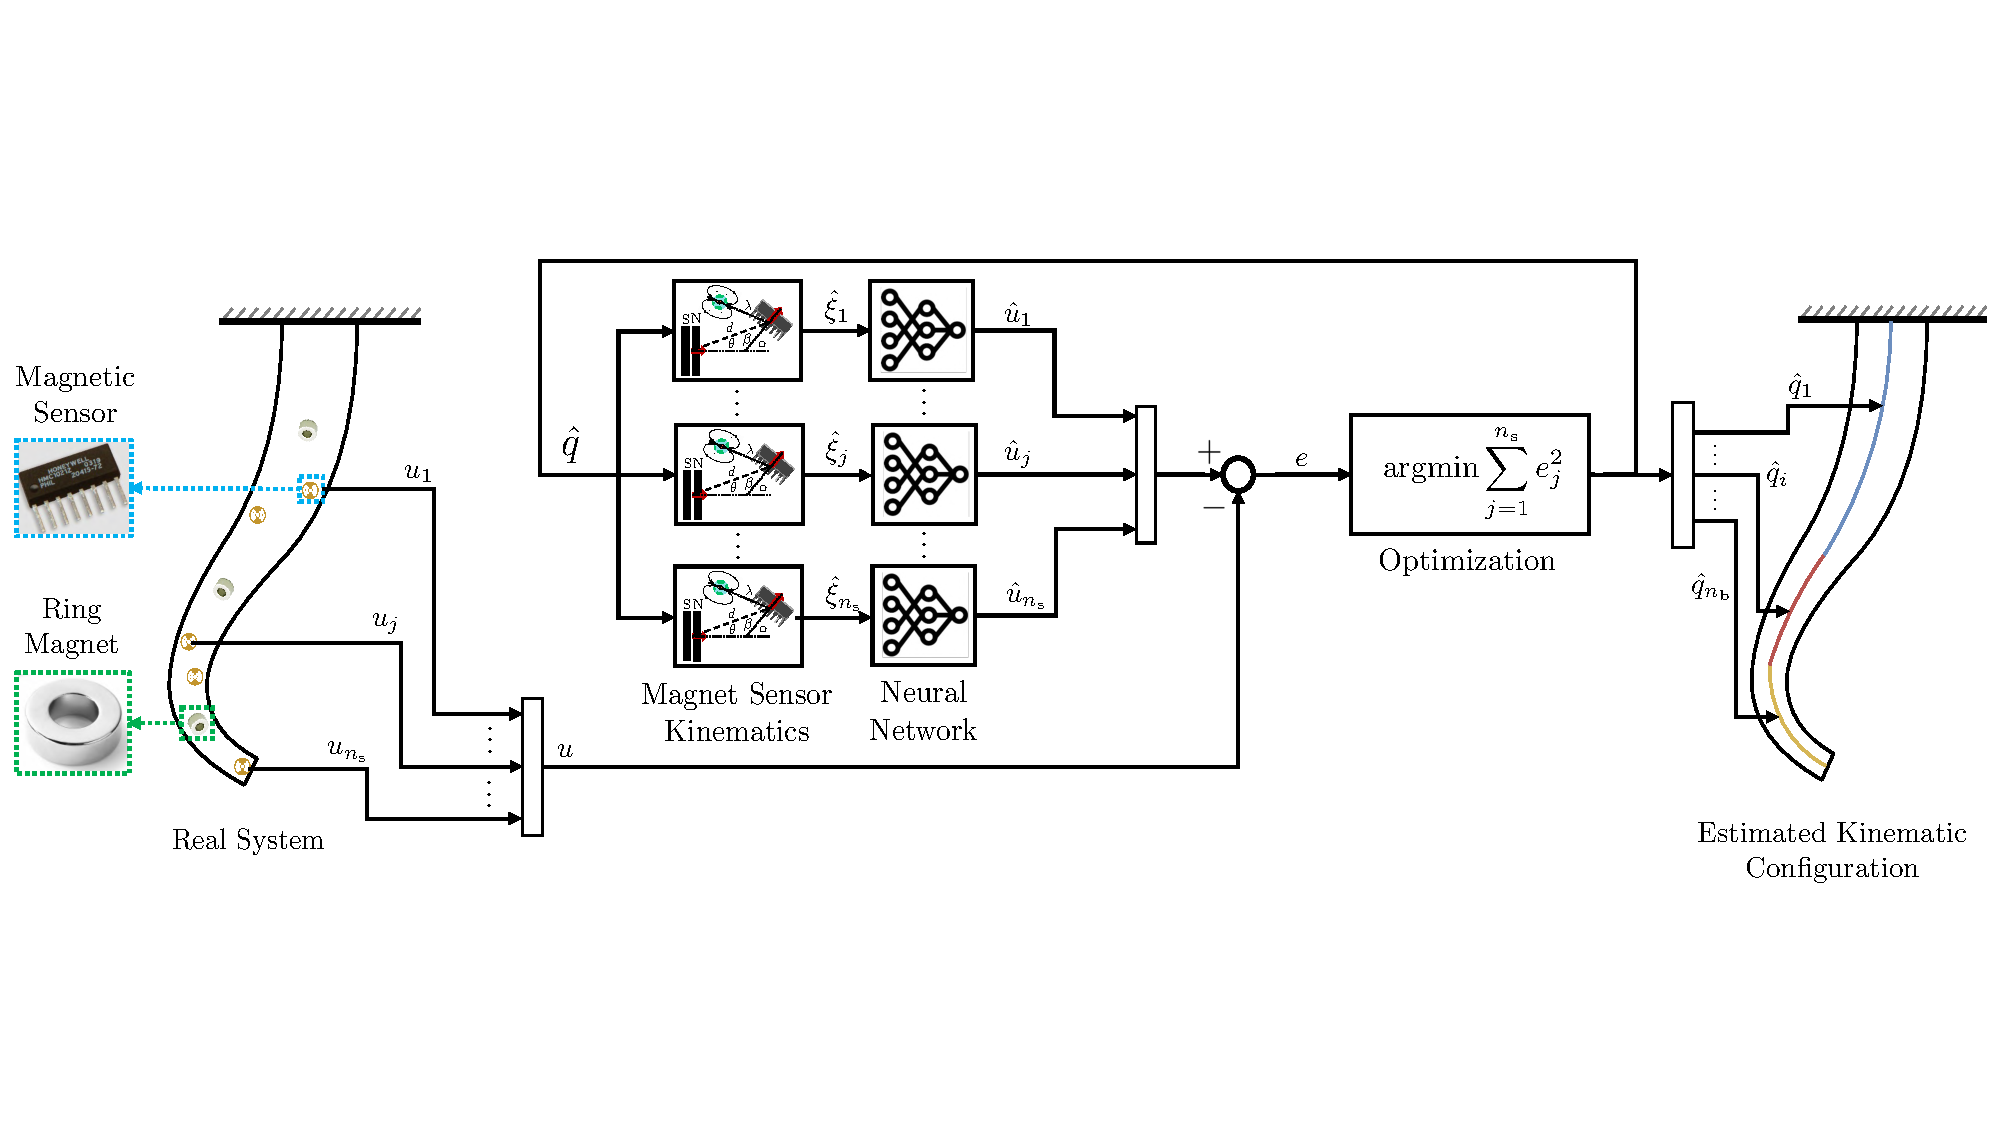
\includegraphics[width=1.0\textwidth]{promasens/figures/methodology/methodology_proprioception_v8_compressed.pdf}
  
  \caption{Proprioception for continuum soft robots with magnetic sensors: an initial configuration estimate $\hat{q}$ is employed to derive the kinematic relationship $\hat{\xi}$ between a sensor and each magnet. Subsequently, this kinematic description is used to predict the sensor measurements $\hat{u} \in \mathbb{R}^{n_\mathrm{s}}$ with a neural network trained in advance. A Mean Squared Error (MSE) metric evaluates the accuracy of the predictions $\hat{u}$ compared to the actual measurements $u$. Finally, we optimize the configuration estimate $\hat{q}$ to achieve proprioception by minimizing the sensor measurement prediction loss.}\label{fig:promasens:methodology}
\end{figure*}

% However, the physical interaction between magnets, sensors, the earth's magnetic field and external disturbances is very complex and highly nonlinear.

% This means that simplified analytical models are usually not sufficient~\cite{ozel2015precise} and inverting the magnetic field equations directly to match sensor measurements with relative locations of the magnet and sensor is intractable~\cite{mitchell2021fast}.

% Related research published by H. Gao et al.~\cite{guo2019continuum} consider a continuum robot made-up of many small sections each containing a magnet and a magnetic sensor. Their approach relies on an analytical model to estimate the 1D bending of small sections of a continuum robot. Subsequently, they fit Quadratic Bézier curves to the curvature of each section to model the shape of the continuum robot.

% An alternative to inaccurate analytical models is to conduct FEA simulations of the magnetic field for the chosen robot design and sensor layout~\cite{ozel2015precise, mitchell2021fast}.

% S. Ozel et al.~\cite{ozel2015precise} leverage Hall effect sensors to measure the curvature of a soft snake-like robot in 2D with both the sensor and magnet directly embedded in the silicon. They rely on data from FEA simulations stored in a look-up table to connect the measured magnetic flux density to translations relative to the magnet. A calibration function derived with least-squares fitting connects the relative translations to the soft robot curvature.

% Along a similar line of work, Mitchell et al.~\cite{mitchell2021fast} follow a probabilistic approach by implementing a particle filter for proprioception with a tri-axis Hall effect sensor. The likelihood weight of each particle is given by the proximity of simulated magnetic flux measurements to the actual measurements.

% All existing approaches rely either on simplified analytical models, which are not suitable for complex geometric arrangements between magnets and sensors, or require to mirror the robot design with all necessary (DoF) in a simulator.

This paper proposes to use permanent ring magnets and multiple magnetic sensors for shape sensing of continuum soft robots. Importantly, we remove the requirement of magnets and sensors being placed in co-axial pairs.
% placed at arbitrary locations within the soft segment. We then present a data-driven approach for making sense of the complex relationship between  measurements - so achieving proprioception with magnetic sensors.
%
We have been inspired by recent work leveraging deep learning to interpret various types of non-magnetic sensor data for proprioception purposes~\cite{truby2020distributed, ding2021predictive, soter2018bodily, thuruthel2019soft}.
% All of them except one~\cite{ding2021predictive} choose Recurrent Neural Network (RNN) structures as their neural network architecture to encourage temporal consistency of the robots' state estimates.
%
However, learning end-to-end mappings from sensors to configurations has three significant drawbacks: (i) it is data-intensive, (ii) it calls for recurrent architectures to encourage temporal consistency for the robot's configuration estimates, (iii) it requires re-training when changing the kinematic model of the robot. We propose a neural architecture that circumvents all three issues (see Fig. \ref{fig:promasens:methodology}).
First, we train shallow neural networks to predict the measurements of the magnetic sensors from a parameterization describing their relative pose with respect to the magnets. We then optimize the configuration estimate - and thus the sensor positions - to minimize the error between the predicted and actual sensor measurements. 
% The result is the robot configuration estimate that better explains the sensor readings. 
This way, we introduce a priori information on the modes of deformation of a continuum soft robot, effectively removing the kinematics from the black box. 
The presented strategy enables us to re-arrange and remove redundant sensors during inference without requiring us to re-train the neural network on the adjusted sensor configuration.
% We provide experiments showing that this architecture achieves a mean precision of \SI{95.5}{\percent} when applied to 3D shape proprioception of a soft segment. 
% Testing on a similar trajectory type as trained on, even an error as low as \SI{1.4}{\percent} is possible.

% However, these existing solutions have some possible drawbacks~\cite{wang2018toward}. The piezoresistive and optical sensors are based over the entire length of the robot. This might result into issues with the robustness of these sensors when the robot has to deform more than the stretchability of the sensors allow. This issue could be resolved with Hall effect sensors, since there is no physical connection between the magnet and the sensor that restricts the robots motion. However, previous papers exploring the use of Hall effect sensors did not consider the estimation of 3D state parametrization.
% %
% This paper proposes a kinematically decoupled, data-driven approach for achieving proprioception with magnetic sensors. We assume the placement of a permanent magnet at the center and multiple magnetoresistive sensors at arbitrary locations within the soft segment.
% Subsequently, we model the kinematic relationship between each magnet and sensor.
% This allows us to remove the kinematics from the black-box and train a neural network to predict the sensor measurements based on a very flexible input description independent of the used state parametrization of the robot.
% An advantage of this explicit kinematic description is that the position of a sensor or magnet can be changed without re-training the entire black-box if the neural network is trained on a sufficient large dataset of kinematic descriptions.
% We employ a loss between the predicted and actual sensor measurements to guide a nonlinear optimization strategy to compute the robot configuration estimate.
% The optimization approach consists of grid search running at lower frequencies in parallel to a fast gradient descent algorithm for local corrections.

% \textcolor{orange}{Do we hypothesize that this reduces the number of trainable parameters?}

% This paper will explore the option to use \gls{MRS} and a permanent magnet, to find a relation between the \gls{MRS} output ans the sensor's position relative to the magnet. Due to the non-linearity of magnetic fields, it is hard to predict this relationship as found in previous 2D applications of similar sensors. Therefore, this paper will look at using \gls{AI} to experimentally link the \gls{MRS} output to a 3D position.
%
% First, a model is needed that captures the position and movement of the robot. For this robot, the \gls{PCC} model is used~\cite{della2020improved}. Subsequently, this model can be used to find the parameters that physically relate the relative position of the magnet and the sensor, the \gls{MSK}. This will be used in combination with a \gls{NN} to predict the sensory output of a single sensor. Afterwards, the error between the predicted sensor output and the measured output is taken. By introducing multiple sensors, a gradient descent can be implemented to descent to the robots configuration by minimizing the error between the predicted and measured sensor values.

To summarize, this paper contributes to the state of the art in soft robot sensing with:
%
\begin{itemize}
    \item A proprioceptive sensing modality relying on multiple magnetic sensors in conjunction with a neural network-based architecture that learns to estimate the full 3D shape of the robot from the sensor readings. % The strategy can deal with small training sets thanks to the injection of kinematic priors.
    % \item A data-driven approach to predict the measurements of \glsp{MRS} integrated into a multi-segment soft robot.
    \item Injection of kinematic priors through a description to spatially relate the poses of a sensor to the magnets. This proposed description serves as an input to a neural network predicting the sensor measurements. %This kinematic description can be easily derived from the \gls{PCC} state description by providing the initial position of magnets and sensors in a straight robot configuration.
    % \item An optimization routine for minimizing the sensor prediction error by running a slow grid search and fast gradient descent in parallel.
    \item Experimental verification of the approach for a one-segment robot with three integrated Magnetoresistive Sensors (MRSs) and proprioception of 3D curvature.    % \item A robust data-driven approach to achieve proprioception for a multi-segment, soft, snake-like robot in 3D.
    %\item Variable and scalable approach to \gls{MRS} measurements.
    % \item Combination of a data-driven sensor measurement model and \gls{MSK} in a gradient descent approach for proprioception.
    % \item Proposing a design how permanent magnets and \glsp{MRS} can be easily integrated into a soft robot.
\end{itemize}
We open-source a Python / PyTorch implementation of the proposed algorithm and the corresponding datasets on GitHub~\footnote{\url{https://www.github.com/tud-cor-sr/promasens}}.

% \begin{figure}[ht]
%     \centering
%     \includegraphics[width=0.575\columnwidth]{promasens/figures/methodology/kinematic_frames_v3_cropped.pdf}
%     \caption{Coordinate frames for a soft segment containing the $j^\mathrm{th}$ magnetic sensor and the $k^\mathrm{th}$ cylindrical magnet placed along the center line. $\{S_{i-1}\}$ and $\{S_{i}\}$ describe the frames of the base and tip of the $i^\mathrm{th}$ segment respectively.}\label{fig:promasens:kinematics_frames_soft_segment}
% \end{figure}

\section{Proprioception with Magnetic Sensors}

This section introduces a methodology to achieve proprioception for soft robots with magnetic sensors.
%
We consider a continuum robot with the shape of its backbone described by the configuration variables $q \in \mathbb{R}^{n_\mathrm{q}}$.
In the commonly used \gls{PCC} kinematic state parametrization~\cite{webster2010design}, the continuum robot is assumed to consist of $n_\mathrm{b}$ segments with each segment exhibiting constant curvature and elongation along its length. Therefore, the configuration of the soft robot can be described with $q \in \mathbb{R}^{3n_\mathrm{b}}$.
Please refer to Appendix~\ref{sub:promasens:kinematic_model_pcc} for more details.
We indeed use PCC for most of our simulations and experiments.
Note, however, that the proposed proprioception algorithm applies to any finite-dimensional kinematic description of a soft robot~\cite{armanini2021soft}.
Indeed, we also specifically consider a robot with affine curvature~\cite{della2020soft, stella2022piecewise_preprint} with its shape described by the configuration $q \in \mathbb{R}^4$. We document this alternative kinematic model in Appendix~\ref{sub:promasens:kinematic_model_ac}.
The proprioception methodology described in the remaining section is agnostic to the chosen kinematic model.
% For the sake of clarity, we use the \gls{PCC} kinematic state parametrization as proposed by \cite{della2020improved}. We consider a continuum robot described by $n_\mathrm{b}$ \gls{CC} segments and configuration variables $q \in \mathbb{R}^{3n_\mathrm{b}}$. Note, however, that the proposed method applies to any finite-dimensional kinematic description of a soft robot~\cite{armanini2021soft}.

\subsection{Proposed method at a glance}

%The shape of each segment can be parameterized with $q_i$.
We integrate $n_\mathrm{m}$ axially symmetric magnets and $n_\mathrm{s}$ magnetic sensors into the robot. The magnets must be installed along the center line of the segment while the sensors can be arbitrarily placed.
%
%To achieve proprioception of the entire robot shape, at least one magnet must be integrated into each segment.
%
Fig.~\ref{fig:promasens:methodology} concisely describes the proposed shape-sensing strategy with a pictorial example of a soft robot described with three constant curvature segments equipped with five magnetic sensors and three cylindrical magnets.
%

The goal of the algorithmic part (center of the figure) is to regress the robot shape (left) by estimating the configuration $\hat{q}$ of all segments (right),
%$q(t) \in \mathbb{R}^{3 n_\mathrm{b}}$
starting from the measurements of the magnetic sensors $u$ (e.g. usually the magnetic flux density).
We achieve this by training a sensor measurement predictor and subsequently optimizing the configuration estimate $\hat{q}$ for the prediction $\hat{u}$ to match the actual sensor measurement $u$.
Instead of predicting the sensor measurements end-to-end, we decouple the kinematics by explicitly describing the kinematic relationship $\hat{\xi}_j = f_{\xi,j}(\hat{q})$ between sensor $j$ and each magnet. % \hat{\xi}_j \in \mathbb{R}^{1+4 n_\mathrm{m}}
Then, we train a neural network $f_{\pi_j}$ to predict the measurement $\hat{u}_j$ based on the input $\hat{\xi}_j$.
To achieve proprioception, we jointly optimize $\hat{q}$ for all sensor measurement predictions. %We define a \gls{MSE} loss between the predicted and actual sensor measurements, and after back-propagating the loss, we perform gradient descent.

% PCC Kinematics with Elongation
% \subsection{Background: Piecewise Constant Curvature Kinematics}\label{sub:promasens:kinematic_model_pcc}

% The state of each segment $i$ of unextended length $L_{0,i}$ and radius $d_i$ is described by
% \begin{equation}\small
%     q_i = \begin{bmatrix}\Delta_{x,i} & \Delta_{y,i} & \delta L_i \end{bmatrix}^{\mathrm{T}} \in \mathbb{R}^3
% \end{equation}
% where $\Delta_{x,i}$ and $\Delta_{y,i}$ represent bending into the local x- and y-directions respectively and $\delta L_i$ defines the extension of the segment.
% The base frame of segment $i$ is referred to as $\{S_{i-1}\}$ as stated in Fig.~\ref{fig:promasens:kinematics_frames_soft_segment}. Given $q_i$, a homogeneous transformation $T_{i-1}^{i}(q_i)$ to the tip frame $\{S_{i}\}$ is available
% \begin{equation}\small
% \label{eq:promasens:transform_improved_q}
% \begin{split}
%     R_{i-1}^{i} &=
%     \begin{bmatrix}
%         1 + \frac{\Delta_{x,i}^2}{\Delta_{i}^2} \left ( \mathrm{c}_i - 1 \right ) & \frac{\Delta_{x,i} \Delta_{y,i}}{\Delta_{i}^2} \left ( \mathrm{c}_i - 1 \right ) & \frac{\Delta_{x,i}}{\Delta_i} \mathrm{s}_i\\
%         \frac{\Delta_{x,i} \Delta_{y,i}}{\Delta_{i}^2} \left ( \mathrm{c}_i - 1 \right ) & 1 + \frac{\Delta_{y,i}^2}{\Delta_{i}^2} \left ( \mathrm{c}_i - 1 \right ) & \frac{\Delta_{y,i}}{\Delta_i} \mathrm{s}_i\\
%         \frac{-\Delta_{x,i}}{\Delta_i} \mathrm{s}_i & \frac{-\Delta_{y,i}}{\Delta_i} \mathrm{s}_i & \mathrm{c}_i
%     \end{bmatrix},\\
%     t_{i-1}^{i} &= \frac{d_i ( L_{0,i}+\delta L_i)}{\Delta_i^2}
%     \begin{bmatrix}
%         \Delta_{x,i} (1 - \mathrm{c}_i) & \Delta_{y,i} (1 - \mathrm{c}_i) & \Delta_{i} \mathrm{s}_i,
%     \end{bmatrix}^{\mathrm{T}}
% \end{split}
% \end{equation}
% where we substituted $\Delta_i = \sqrt{\Delta_{x,i}^2 + \Delta_{y,i}^2}$, $\mathrm{s}_i = \sin \left ( \frac{\Delta_i}{d_i} \right )$, and $\mathrm{c}_i = \cos \left ( \frac{\Delta_i}{d_i} \right )$ for conciseness.

\begin{figure}[t]
\centering
\subfigure[Magnet Sensor Kinematics]{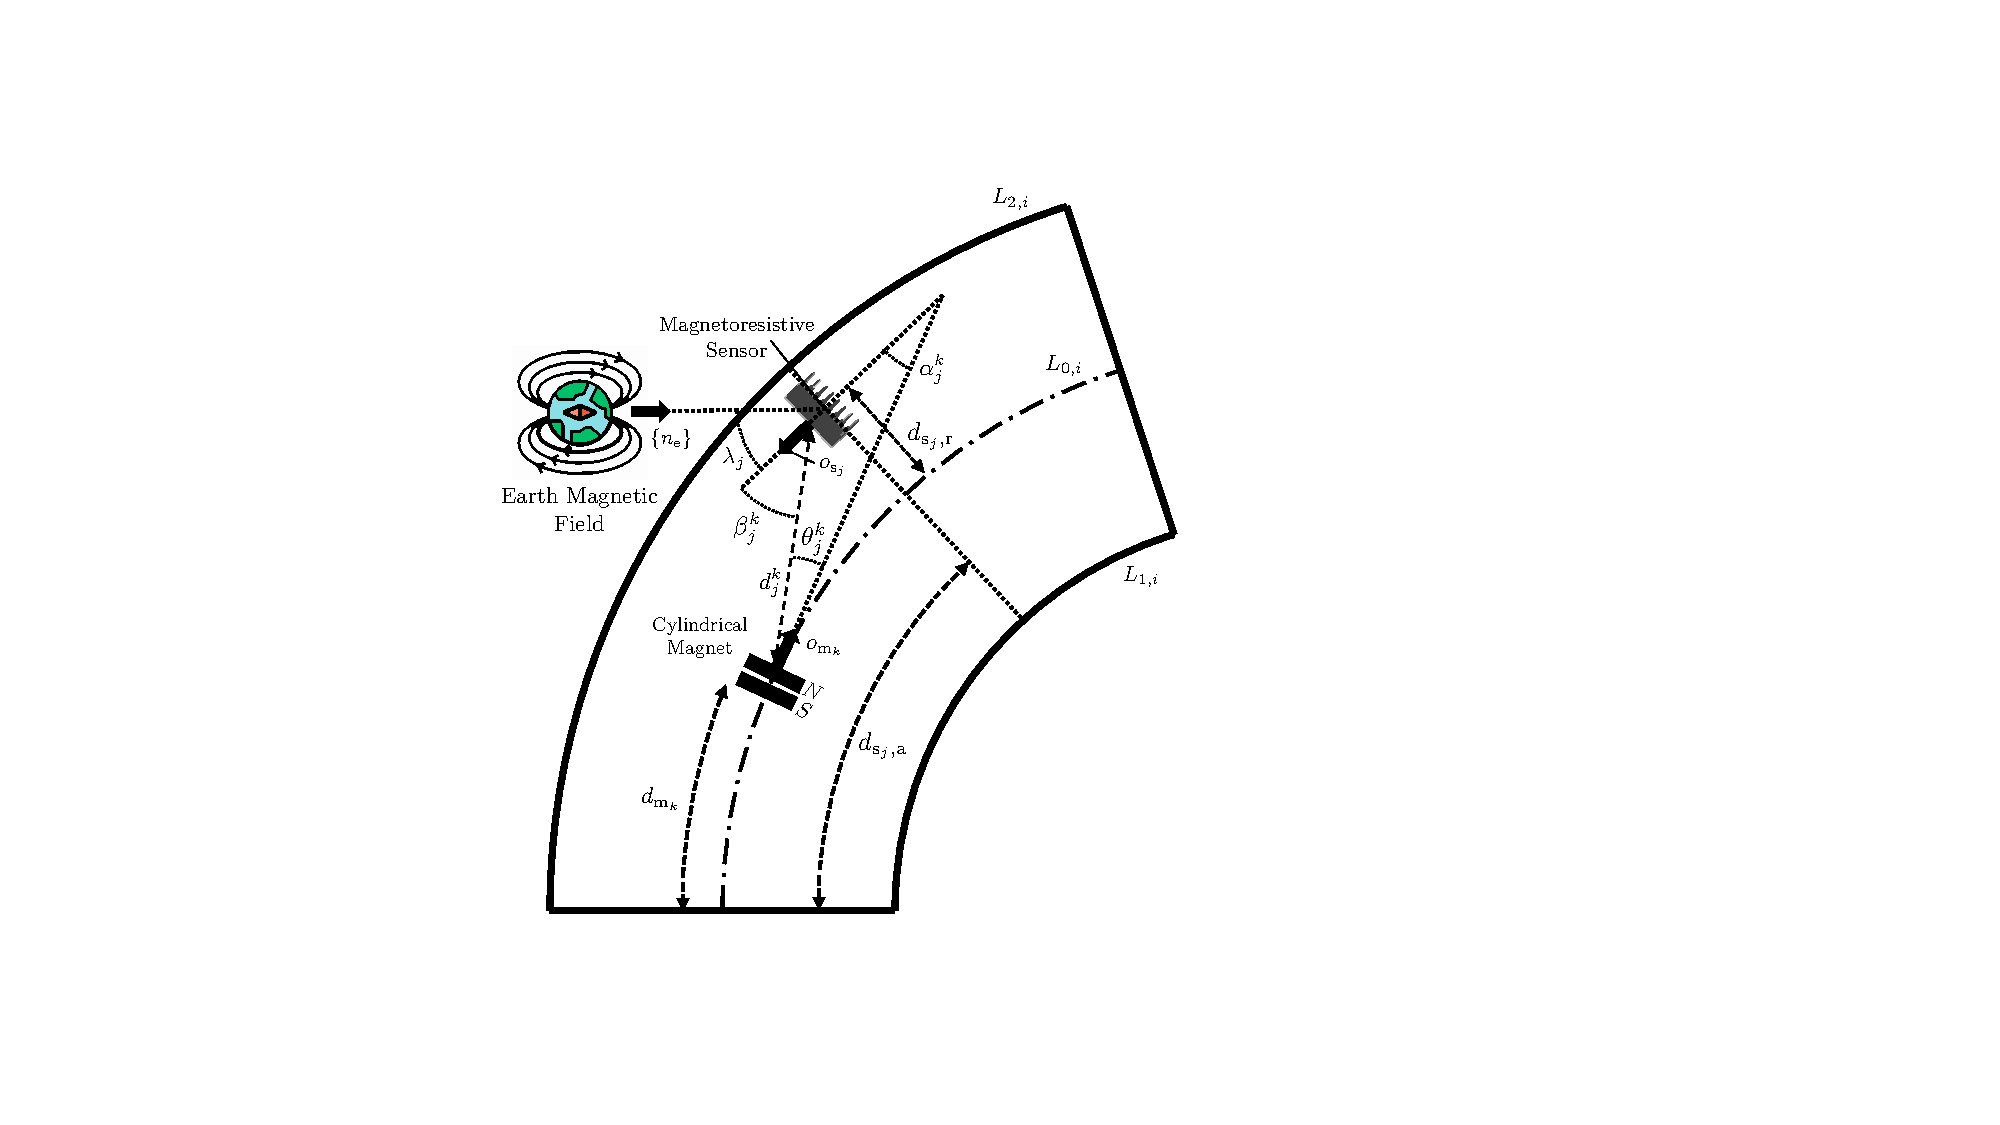
\includegraphics[width=0.5\columnwidth]{promasens/figures/methodology/magnet_sensor_kinematics_v5_compressed.pdf}\label{fig:promasens:magnet_sensor_kinematic}}
\subfigure[Coordinate transformations]{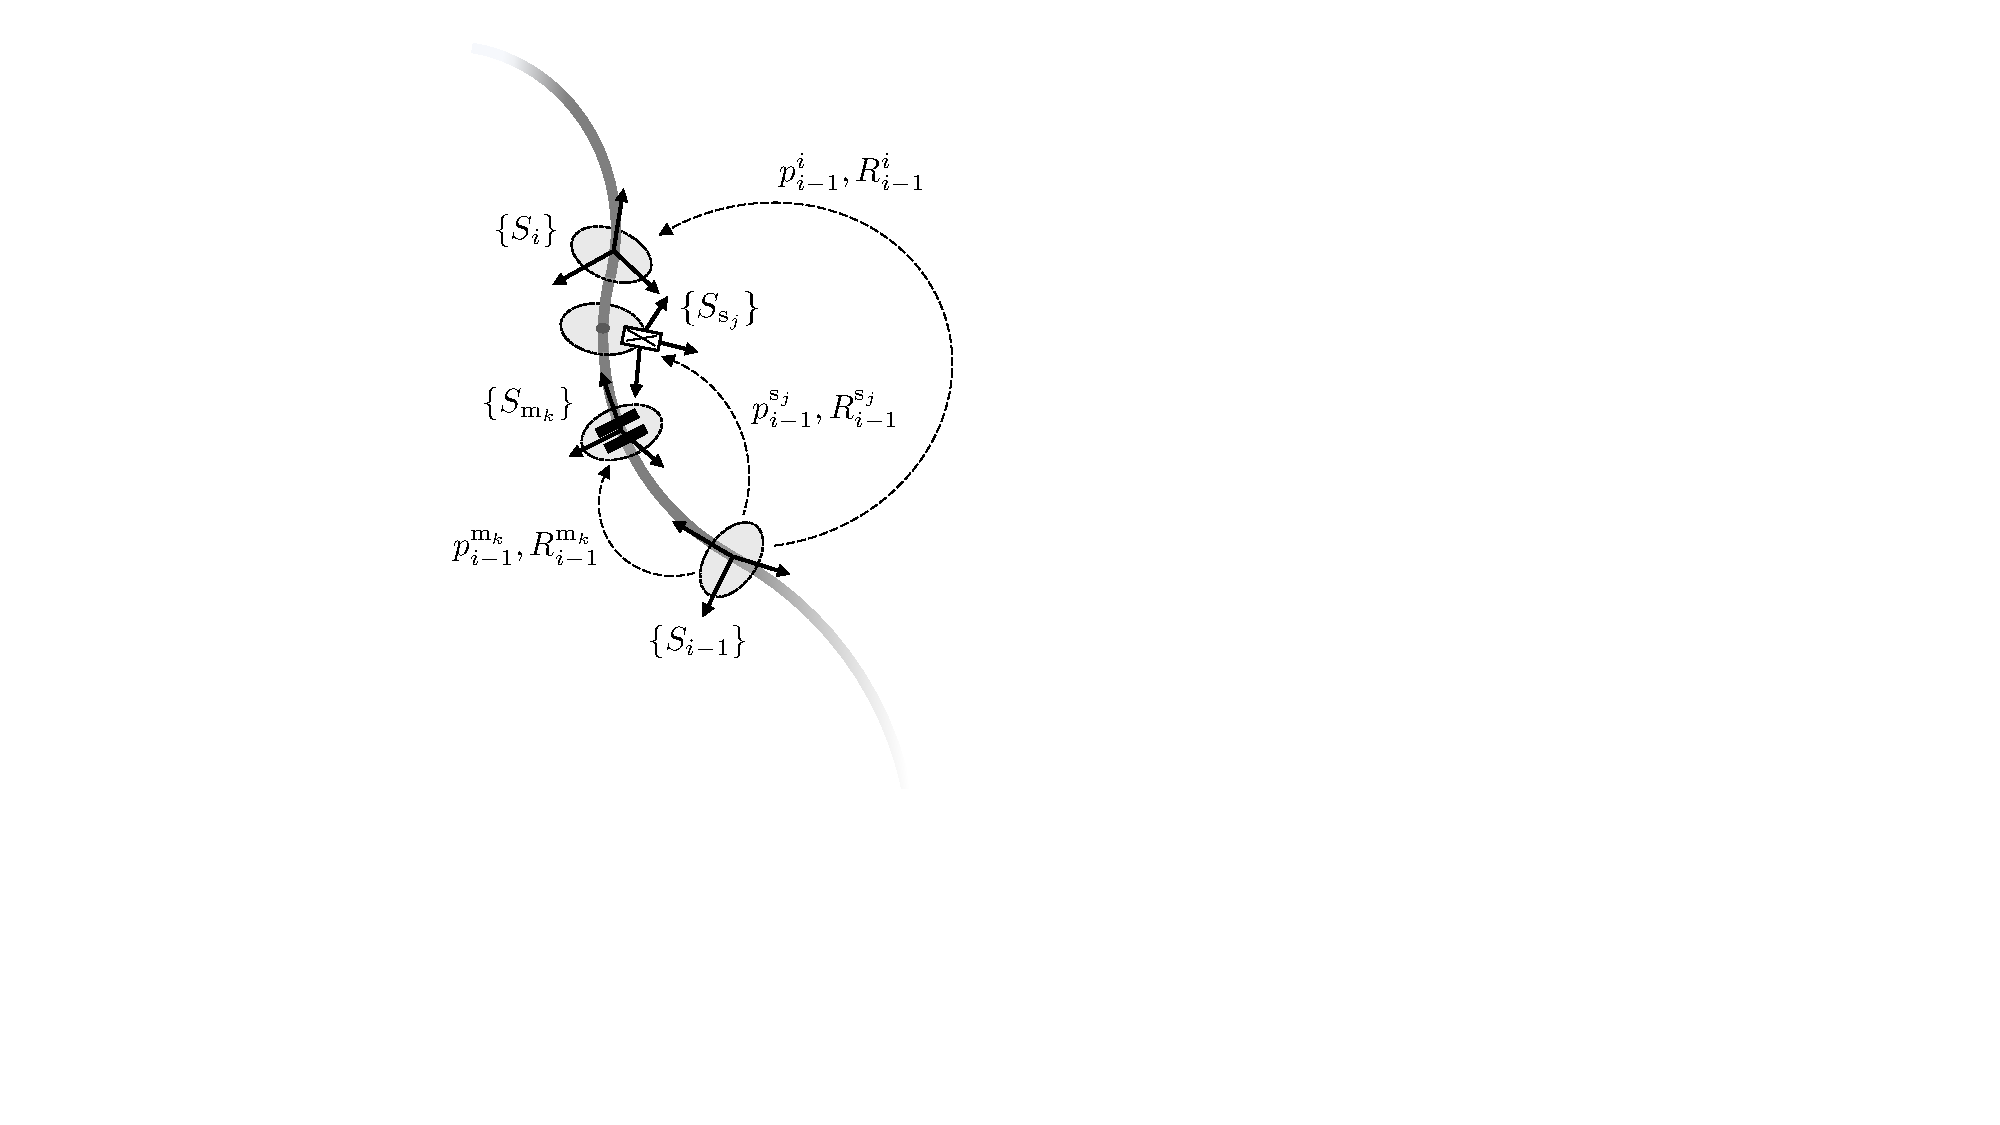
\includegraphics[width=0.4\columnwidth]{promasens/figures/methodology/kinematic_frames_v5_cropped.pdf}\label{fig:promasens:kinematics_frames_soft_segment}}
\caption{\textbf{Panel (a):} Parameters used to describe the kinematics between the $j^\mathrm{th}$ sensor and the $k^\mathrm{th}$ magnet. To simplify the illustration, we visualize the unextended planar case with both magnet and sensor part of the $i^\mathrm{th}$ segment. However, this is not a strict assumption as magnets and sensors can also be part of different segments. \textbf{Panel (b):} Coordinate frames for a soft segment containing the $j^\mathrm{th}$ magnetoresistive sensor and the $k^\mathrm{th}$ cylindrical magnet placed along the center line. $\{S_{i-1}\}$ and $\{S_{i}\}$ describe the frames of the base and tip of the $i^\mathrm{th}$ segment, respectively.}
\end{figure}

\section{Background: Continuum soft robot kinematics}\label{sec:promasens:kinematics}
A kinematic description provides us with the forward kinematic transformation $T_{i-1}^s(q_i,s)$ from base frame $\{S_{i-1}\}$ at the proximal end of the $i^\mathrm{th}$ segment to the local frame $\{S_{v}\}$ at a coordinate $v \in [0,1]$ for a given configuration $q_i$. Furthermore, the tip frame of the $i^\mathrm{th}$ segment located at the coordinate $v = 1$ is denoted as $\{S_{i}\}$, as shown in Fig.~\ref{fig:promasens:kinematics_frames_soft_segment}.

\subsection{$\Delta$-parametrization of the piecewise constant curvature kinematics}\label{sub:promasens:kinematic_model_pcc}
% \section*{Appendix: $\Delta$-parametrization of the Piecewise Constant Curvature Kinematics}\label{sub:promasens:kinematic_model_pcc}

Under the \gls{PCC} hypothesis, the shape of each segment $i$ of length $L_{i}$ and radius $d_i$ can be fully parameterized through three variables
\begin{equation}\small
    q_i = \begin{bmatrix}\Delta_{x,i} & \Delta_{y,i} & \delta L_{i} \end{bmatrix}^{\mathrm{T}} \in \mathbb{R}^3
\end{equation}
where $\Delta_{x,i}$ and $\Delta_{y,i}$ represent bending into the local $x$ and $y$ directions respectively and $\delta L_i$ defines the elongation of the segment.
The base frame of segment $i$ is referred to as $\{S_{i-1}\}$ as stated in Fig.~\ref{fig:promasens:kinematics_frames_soft_segment}. Given $q_i$, a homogeneous transformation $T_{i-1}^{v}(q_i, v)$ to the point frame $\{S_{v}\}$ is available
\begin{equation}\small
\label{eq:promasens:transform_improved_q}
\begin{split}
    R_{i-1}^{v}(q_i,v) &=
    \begin{bmatrix}
        1 + \frac{\Delta_{x,i}^2}{\Delta_{i}^2} \left ( \mathrm{C}_v - 1 \right ) & \frac{\Delta_{x,i} \Delta_{y,i}}{\Delta_{i}^2} \left ( \mathrm{C}_v - 1 \right ) & \frac{\Delta_{x,i}}{\Delta_i} \mathrm{S}_v\\
        \frac{\Delta_{x,i} \Delta_{y,i}}{\Delta_{i}^2} \left ( \mathrm{C}_v - 1 \right ) & 1 + \frac{\Delta_{y,i}^2}{\Delta_{i}^2} \left ( \mathrm{C}_v - 1 \right ) & \frac{\Delta_{y,i}}{\Delta_i} \mathrm{S}_v\\
        \frac{-\Delta_{x,i}}{\Delta_i} \mathrm{S}_v & \frac{-\Delta_{y,i}}{\Delta_i} \mathrm{S}_v & \mathrm{C}_v
    \end{bmatrix},\\
    p_{i-1}^{i}(q_i,v) &= \frac{d_i ( L_{0,i}+\delta L_i)}{v \, \Delta_i^2}
    \begin{bmatrix}
        \Delta_{x,i} (1 - \mathrm{C}_v) & \Delta_{y,i} (1 - \mathrm{C}_v) & \Delta_{i} \mathrm{S}_v,
    \end{bmatrix}^{\mathrm{T}}
\end{split}
\end{equation}
where $R_{i-1}^{v}$, $p_{i-1}^{i}(q_i,v)$ denote the rotation matrix and translation vector respectively. We substituted $\Delta_i = \sqrt{\Delta_{x,i}^2 + \Delta_{y,i}^2}$, $\mathrm{S}_v = \sin \left (\frac{v \, \Delta_i}{d_i} \right )$, and $\mathrm{C}_v = \cos \left ( \frac{v \, \Delta_i}{d_i} \right )$ for conciseness.

\subsection{Affine curvature kinematics}\label{sub:promasens:kinematic_model_ac}
The affine curvature hypothesis~\cite{della2020soft, stella2022piecewise_preprint} models the bending of the soft segment to be conforming to the affine function $\kappa(t,v) = \kappa_0(t) + \kappa_1(t) v$, where $\kappa$ describes the local curvature of the backbone at the coordinate $v \in [0, 1]$ along the segment and $\kappa_0(t)$, $\kappa_1(t)$ are the zero-order and first-order term of the curvature polynomial respectively~\cite{della2019control}.
Specifically, we implement the recently proposed extension to 3D environments~\cite{stella2022piecewise_preprint}, which specifies an azimuth angle of the bending direction $\phi(t)$ and additionally allows for an elongation $\delta L(t)$ of the segment.
% We extend this parametrization as introduced by Della Santina et al.~\cite{della2019control, della2020soft} to 3D environments by specifying the azimuth angle of the bending direction $\phi(t)$ and additionally allowing for an elongation $\delta L(t)$ of the segment. 
Accordingly, the configuration of the $i^\mathrm{th}$ segment is described at any point in time by
\begin{equation}\small
    q_i = \begin{bmatrix}\kappa_{0,i} & \kappa_{1,i} & \phi_i & \delta L_{i} \end{bmatrix}^{\mathrm{T}} \in \mathbb{R}^4.
\end{equation}
Now that the configuration space is defined, we aim to find a description of the forward kinematics. Firstly, the bending angle $\theta_i(q, v)$ is found by integrating the curvature
\begin{equation}\small
    \theta(q,v) = \int_{v'=0}^{v} \kappa_i(q, v') \, \mathrm{d}v' = \kappa_{0,i} \, v + \kappa_{1,i} \, \frac{v^2}{2}.
\end{equation}
The rotation to the frame $\{S_{v}\}$ can then be easily determined with $R_{i-1}^{i}(q,v) = R_{\phi_i}(q,v) \, R_{\theta}(q,v) R_{\phi_i}^\mathrm{T}(q,v)$. After substituting $S_{\cdot} = \sin(\cdot)$, $C_{\cdot} = \cos(\cdot)$ for conciseness, we state the homogeneous transformation as
\begin{equation}\small\label{eq:promasens:affine_curvature_forward_kinematics}
\begin{split}
    R_{i-1}^v(q,v) &= \begin{bmatrix}
        S_{\phi_i}^2 C_{\theta_v} + C_{\phi_i}^2 & -S_{\phi_i} C_{\phi_i} C_{\theta_i} + S_{\phi_i}C_{\phi_i} & S_{\phi_i} S_{\theta_v}\\
        -S_{\phi_i} C_{\phi_i} C_{\theta_i} + S_{\phi_i} C_{\phi_i} & S_{\phi_i}^2 + C_{\phi_i}^2 C_{\theta_v} & -S_{\theta_v} C_{\phi_i}\\
        -S_{\phi_i} S_{\theta_v} & S_{\theta_v} C_{\phi_i} & C_{\theta_i}
    \end{bmatrix},\\
    p_{i-1}^{v}(q,v) &= \left ( L_{0,i} + \delta L_i \right ) \, \begin{pmatrix}
        \int_{v'=0}^{v} \sin(\theta(q, v')) \, \mathrm{d}v' \, \sin(\phi_i)\\
        - \int_{v'=0}^{v} \sin(\theta(q, v')) \, \mathrm{d}v' \, \cos(\phi_i)\\
        \int_{v'=0}^{v} \cos(\theta(q, v')) \, \mathrm{d}v'
    \end{pmatrix}.
\end{split}
\end{equation}
We choose to integrate the translational terms in \eqref{eq:promasens:affine_curvature_forward_kinematics} numerically with $101$ sample points using the Torchquad~\cite{gomez2021torchquad} implementation of the Simpson's rule, which makes the forward kinematics fully and automatically differentiable.


\subsection{Magnet sensor kinematics}\label{sub:promasens:kinematic_model_magnet_sensor_kinematics}
This subsection derives the kinematic relationship $\xi_j = f_{\xi_j}(q) \in \mathbb{R}^{1+4n_\mathrm{m}}$ between the $j^\mathrm{th}$ sensor and all $n_\mathrm{m}$ magnets as we hypothesize that we can estimate the sensor measurement $u_j$ solely based on
a) the angle $\lambda_j \in \mathbb{R}^1$ to the earth's magnetic field,
b) the distance $d_j^k$  between the $j^\mathrm{th}$ sensor and $k^\mathrm{th}$ magnet,
c) the angle $\alpha_j^k$ between the sensor measurement direction and the cylindrical axis of the magnet,
d) the angle $\beta_j^k$ between the sensor measurement direction and the vector from the magnet to the sensor,
and e) the angle $\theta_j^k$ between the cylindrical axis of the magnet and the vector from the magnet to the sensor.
Accordingly, $\xi_j$ is defined as
\begin{equation}\small
    \xi_{j} = f_{\mathrm{\xi},j}(q) =
    \begin{pmatrix}
        \lambda_{j} & {\xi_{j}^1}^\mathrm{T} & \cdots & {\xi_{j}^k}^\mathrm{T} & \cdots & {\xi_{j}^{n_\mathrm{m}}}^\mathrm{T}
    \end{pmatrix}^\mathrm{T} \in \mathbb{R}^{1 + 4n_\mathrm{m}},
\end{equation}
with $\xi_j^{k} \in \mathbb{R}^4$ the kinematic relationship between the $j^\mathrm{th}$ sensor and the $k^\mathrm{th}$ magnet: $\xi_j^{k} = \begin{pmatrix} d_j^k & \alpha_j^k & \beta_j^k & \theta_j^k \end{pmatrix}^\mathrm{T} \in \mathbb{R}^4$. We visualize the parameters incorporated in $\xi_j^{k}$ in Fig.~\ref{fig:promasens:magnet_sensor_kinematic}.
% \begin{equation}\small
%     \xi_j^{k} = \begin{pmatrix} d_j^k & \alpha_j^k & \beta_j^k & \theta_j^k \end{pmatrix}^\mathrm{T}.
% \end{equation}

In the following, we present the derivation of all components of $\xi_j^{k}$. 
Please note that all kinematic frames used in the following paragraphs are visualized in Fig.~\ref{fig:promasens:kinematics_frames_soft_segment}.
% \textcolor{blue}{All the kinematic frames introduced over the last few paragraphs are visualized in Fig.~\ref{fig:promasens:kinematics_frames_soft_segment}}.

We define that the $k^\mathrm{th}$ magnet is integrated into the $i^\mathrm{th}$ segment. Now, we first derive a transformation matrix $T_{i-1}^{\mathrm{m}_k}$ from the base frame $\{S_{i-1}\}$ to the magnet frame $\{ S_{\mathrm{m}_k} \}$. 
This can be achieved by evaluating the chosen kinematic model, two of which we report in the Appendix~\ref{appx:kinematics}, at the segment coordinate $v = \frac{d_{\mathrm{m}_k}}{L_{0,i}}$. 
This means that the cylindrical magnet is integrated at a distance, which is measured along the backbone, of $d_{\mathrm{m}_k}$ from the base of the segment.
% The cylindrical magnet is integrated into the segment at an axial distance of $d_{\mathrm{m}_k}$ from $\{S_{i-1}\}$.
% We compute the translational and rotational components of the transformation matrix $p_{i-1}^{\mathrm{m}_k}$ and $R_{i-1}^{\mathrm{m}_k}$ \textcolor{blue}{by evaluating the forward kinematics $T_{i-1}^v(q_i,v)$, which are reported in Appendix~\ref{appx:kinematics}, at the point $v = \frac{d_{\mathrm{m}_k}}{L_{0,i}}$.}

% as in \cite{della2020improved} by substituting $\Delta_{x}^{\mathrm{m}_k} = \frac{d_{\mathrm{m}_k}}{L_{0,i}} \, \Delta_{x,i}$, $\Delta_{y}^{\mathrm{m}_k} = \frac{d_{\mathrm{m}_k}}{L_{0,i}} \, \Delta_{y,i}$ and $\Delta_{\mathrm{m}_k} = \frac{d_{\mathrm{m}_k}}{L_{0,i}} \, \Delta_{i}$. % in \eqref{eq:promasens:transform_improved_q}.

Subsequently, we  describe the pose of the $j^\mathrm{th}$ sensor with respect to the base of the $i^\mathrm{th}$ segment.
Denote with $d_{\mathrm{s}_j,\mathrm{r}}$ the radial distance of the sensor from the center line, with $\varphi_j$ the azimuth angle of the sensor in the cylindrical plane, and with $d_{\mathrm{s}_j,\mathrm{a}}$ the axial distance along the center line from the base of the $i^\mathrm{th}$ segment.
We derive the transformation $T_{i-1}^{\mathrm{s}_j,\mathrm{r}_0}$ to the center of the cylindrical plane of the sensor % using \eqref{eq:promasens:transform_improved_q}
analogously as for the magnets by evaluating the forward kinematics at $v = \frac{d_{\mathrm{s}_j,\mathrm{a}}}{L_{0,i}}$.
% by scaling the configuration vector $q_i$ with $\frac{d_{\mathrm{s}_j,\mathrm{a}}}{L_{0,i}}$ in the transformation matrix~\cite{della2020improved}.
This is followed by applying the radial offset $d_{\mathrm{s}_j,\mathrm{r}}$ in the cylindrical plane of the sensor
% \begin{equation}\small
% \begin{split}
%     t_{i-1}^{\mathrm{s}_j} = t_{i-1}^{\mathrm{s}_j,\mathrm{r}_0} + R_{i-1}^{\mathrm{s}_j,\mathrm{r}_0} \, d_{\mathrm{s}_j,\mathrm{r}}
%     \,
%     \begin{pmatrix}
%         \cos{\varphi_j} & \sin{\varphi_j} & 0
%     \end{pmatrix}^{\mathrm{T}}.
% \end{split}
% \end{equation}
\begin{equation}\small
    T_{i-1}^{\mathrm{s}_j} = T_{i-1}^{\mathrm{s}_j,\mathrm{r}_0}
    \,
    \begin{bmatrix}
        \cos{\varphi_j} & - \sin{\varphi_j} & 0 & d_{\mathrm{s}_j} \cos(\varphi_j)\\
        \sin{\varphi_j} & \cos{\varphi_j} & 0 & d_{\mathrm{s}_j} \sin(\varphi_j)\\
        0 & 0 & 1 & 0\\
        0 & 0 & 0 & 1\\
    \end{bmatrix}.
\end{equation}
Optionally, a static rotation offset can be applied to $R_{i-1}^{\mathrm{s}_j}$ such that local z-axis $\{ o_{\mathrm{s}_j} \}$ corresponds to the sensor measurement direction.
% Hereafter, we will assume that the measurement direction of the sensor points along the local positive  z-axis and any other orientation is compensated by adding a static rotation offset to $R_{i-1}^{\mathrm{s}_j}$.

Knowing the transformation matrices from the base frame of the respective segment to the sensor and magnet frames, we express them in the inertial frame $\{S_{0}\}$ by multiplying with the kinematic chain $T_{0}^{i-1} = \Pi_{\bar{i}=1}^{i-1} \, T_{\bar{i}-1}^{\bar{i}}$.

Next, we need to express the sensor measurement direction $\{ o_{\mathrm{s}_j} \}_{0}$ and the cylindrical axis of the magnet $\{ o_{\mathrm{m}_k} \}_{0}$ in the inertial frame
\begin{equation}\small
    \{ o_{\mathrm{s}_j} \}_{0} = R_{0}^{\mathrm{s}_j}
    \begin{pmatrix}
        0 & 0 & 1
    \end{pmatrix}^{\mathrm{T}},
    \quad
    \{ o_{\mathrm{m}_k} \}_{0} = R_{0}^{\mathrm{m}_k}
    \begin{pmatrix}
        0 & 0 & 1
    \end{pmatrix}^{\mathrm{T}}.
\end{equation}
% and analogue for the cylindrical axis of the magnet $\{ \hat{o}_{\mathrm{m}_k} \}_{0}$
% \begin{equation}\small
%     \{ \hat{o}_{\mathrm{m}_k} \}_{0} = R_{0}^{\mathrm{m}_k}
%     \begin{pmatrix}
%         0 & 0 & 1
%     \end{pmatrix}^{\mathrm{T}}.
% \end{equation}
%
As the sensor measures contributions of the earth's magnetic field, we need to state the angle $\lambda_{j}$ between $\{ o_{\mathrm{s}_j} \}_0$ and the earth's magnetic field unit vector $\{ n_{\mathrm{e}} \}_{0}$. 
Similarly, we investigate the angle $\alpha_j^k$ between $\{ o_{\mathrm{s}_j} \}_{0}$ and the cylindrical axis of the magnet $\{ o_{\mathrm{m}_k} \}_{0}$
\begin{equation}\small
    \cos (\lambda_{j}) = \{n_{\mathrm{e}} \}_{0} \cdot \{ o_{\mathrm{s}_j} \}_{0},
    \quad
    \cos (\alpha_{j}^k) = \{ o_{\mathrm{m}_k} \}_{0} \, \{ o_{\mathrm{s}_j} \}_{0}.
\end{equation}
% While $\{ \hat{n}_{\mathrm{e}} \}_{0}$ is dependent on the exact experimental setup, we report for the special case of the z-axis of the $\{S_{0}\}$ frame being perpendicular to the earth surface with a compass displaying an angle of $\varphi_e$ to the x-axis the following relation
% \begin{equation}\small
%     \{ \hat{n}_{\mathrm{e}} \}_{0} =
%     \begin{pmatrix}
%         \cos(\varphi_e) & \sin(\varphi_e) & 0
%     \end{pmatrix}^{\mathrm{T}}.
% \end{equation}
% Next, we investigate the angle $\alpha_j^k$ between the sensor measurement direction $\{ \hat{o}_{\mathrm{s}_j} \}_{0}$ and the cylindrical axis of the magnet $\{ \hat{o}_{\mathrm{m}_k} \}_{0}$
% \begin{equation}\small
%     \cos (\alpha_{j}^k) = \{ \hat{o}_{\mathrm{m}_k} \}_{0} \, \{ \hat{o}_{\mathrm{s}_j} \}_{0}.
% \end{equation}
We define the translation and distance between the magnet and the sensor in the frame $\{S_{0}\}$ as:
\begin{equation}\small\label{eq:promasens:t_jk_and_d_jk}
    p_j^{k} = p_{0}^{\mathrm{s}_j} - p_{0}^{\mathrm{m}_k}, \qquad  d_j^k = \lVert p_{j}^{k} \rVert_2.
\end{equation}
% This lets us find the distance between the sensor and the magnet with the Euclidean norm
% \begin{equation}\label{eq:promasens:d_jk}\small
%     d_j^k = \lVert t_{j}^{k} \rVert_2.
% \end{equation}
Building on the derivation in \eqref{eq:promasens:t_jk_and_d_jk}, we compute the angles $\beta_j^k$ and $\theta_j^k$ using the dot product rule
\begin{equation}\label{eq:promasens:theta_jk_and_beta_jk}\small
    \cos (\beta_j^k) = \frac{p_j^{k} \, \{ o_{\mathrm{s}_j} \}_{0}}{\lVert p_j^{k} \rVert}_2,
    \qquad
    \cos (\theta_j^k) = \frac{p_j^{k} \, \{ o_{\mathrm{m}_k} \}_{0}}{\lVert p_j^{k} \rVert}_2.
\end{equation}
Lastly, the kinematic descriptions for all sensors are vertically stacked as
\begin{equation}\small
    \xi = \begin{pmatrix} \xi_1^\mathrm{T} \dots \xi_j^\mathrm{T} \dots \xi_{n_\mathrm{s}}^\mathrm{T} \end{pmatrix}^\mathrm{T} \in \mathbb{R}^{n_\mathrm{s} + 4n_\mathrm{m} n_\mathrm{s}}.
\end{equation}
% $\xi_j(t) \in \mathbb{R}^{1 + 4n_\mathrm{m}}$
% $\xi(t) = f_\xi(q(t)) \in \mathbb{R}^{n_\mathrm{s} + 4n_\mathrm{m} n_\mathrm{s}}$
We will in the following refer to the mapping $f_\xi(q): q \in \mathbb{R}^{n_\mathrm{q}}
\rightarrow \xi \in \mathbb{R}^{n_\mathrm{s} + 4n_\mathrm{m} n_\mathrm{s}}$ as the magnet sensor kinematics.


% \begin{algorithm}[hbt!]
% \caption{Proprioception with magnetic sensors}\label{alg:proprioception}
% \begin{algorithmic}
% \REQUIRE $u(t) \in \mathbb{R}^{n_\mathrm{s}}$ \COMMENT{Sensor measurements}
% \STATE  \hspace{7mm} $\hat{q}(t-1) \in \mathbb{R}^{3n_\mathrm{b}}$
% \COMMENT{Configuration of prev. time-step}
% \STATE  \hspace{7mm} $\hat{q}_\mathrm{glob}^*(t-\delta) \in \mathbb{R}^{3n_\mathrm{b}}$
% \COMMENT{Solution of grid search $\delta$ ago}
% \STATE  \hspace{7mm} $f_\xi: \mathbb{R}^{2n_\mathrm{b}} \rightarrow \mathbb{R}^{n_\mathrm{s} + 4n_\mathrm{m} n_\mathrm{s}}$ \COMMENT{Magnet Sensor Kin.}
% \STATE  \hspace{7mm} $f_\pi: \mathbb{R}^{n_\mathrm{s} + 4n_\mathrm{m} n_\mathrm{s}} \rightarrow \mathbb{R}^{n_\mathrm{s}}$ \COMMENT{Trained neural network}
% \ENSURE $\hat{q}(t) \in \mathbb{R}^{2n_\mathrm{b}}$ \COMMENT{Estimated robot configuration}
%     \IF{gridSearchIsFinished()}
%         \STATE $\hat{q}_0 \gets \hat{q}_\mathrm{glob}^*(t-\delta)$
%     \ELSE
%         \STATE $\hat{q}_0 \gets \hat{q}(t-1)$
%     \ENDIF
%     \vspace{0.25em}
%     \STATE $l \gets 0$
%     \STATE $b_l \gets 0 \in \mathbb{R}^{3n_\mathrm{b}}$
%     \vspace{0.25em}
%     % \WHILE{$\left|\Omega \right| >\epsilon$}
%     \WHILE{$l < n_\mathrm{it}$}
%     \vspace{0.25em}
%     \STATE $\hat{\xi}_l \gets f_{\xi}(\hat{q}_{l})$
%     \vspace{0.25em}
%     \STATE $\hat{u}_l \gets f_\pi(\hat{\xi}_l)$
%     \vspace{0.25em}
%     \STATE $\hat u_{l}^{\mathrm{error}} \gets \lVert \hat{u}_{l}-u(t) \rVert_2$
%     \vspace{0.25em}
%     % \STATE $\frac{\partial}{\partial \hat{q}_l} \mathcal{L}_{u}(\hat{q}_l) \gets \frac{2}{n_\mathrm{s}} \frac{\partial }{\partial {\hat{q}_l}} f_{\mathrm{\xi}}^\mathrm{T}(\hat{q}_l) \, \frac{\partial}{\partial {\hat{\xi}_l}} f_\pi^\mathrm{T}(\hat{\xi}_l) \, (\hat{u}_l - u(t))$
%     \STATE $b_{l+1} \gets \mu \, b_l + \frac{2}{n_\mathrm{s}} \frac{\partial }{\partial {\hat{q}_l}} f_{\mathrm{\xi}}^\mathrm{T}(\hat{q}_l) \, \frac{\partial}{\partial {\hat{\xi}_l}} f_\pi^\mathrm{T}(\hat{\xi}_l) \, (\hat{u}_l - u(t))$
%     % \vspace{0.25em}
%     \STATE $\hat{q}_{l+1} \gets \hat{q}_l - \gamma \, b_{l+1} $
%     % \vspace{0.25em}
%     % \textcolor{orange}{\STATE $ \Omega \gets \mathrm{RMSE}(\hat{u}_{l+1}^{error})-\mathrm{RMSE}(\hat{u}_{l-n_\mathrm{p}}^{error})$ \COMMENT{Early Stopping Criteria with patience $n_\mathrm{p}$}}
%     \vspace{0.25em}
%     \STATE $l \gets l + 1$
% \ENDWHILE
% \STATE $l^* \gets \mathrm{argmin}_{l} \, u_{l}^{error}$
% \STATE $\hat{q}(t) \gets \hat{q}_l^{*}$
% \end{algorithmic}
% \end{algorithm}

\begin{figure}[ht]
\centering
    % \subfigure[Optimization scheduling]{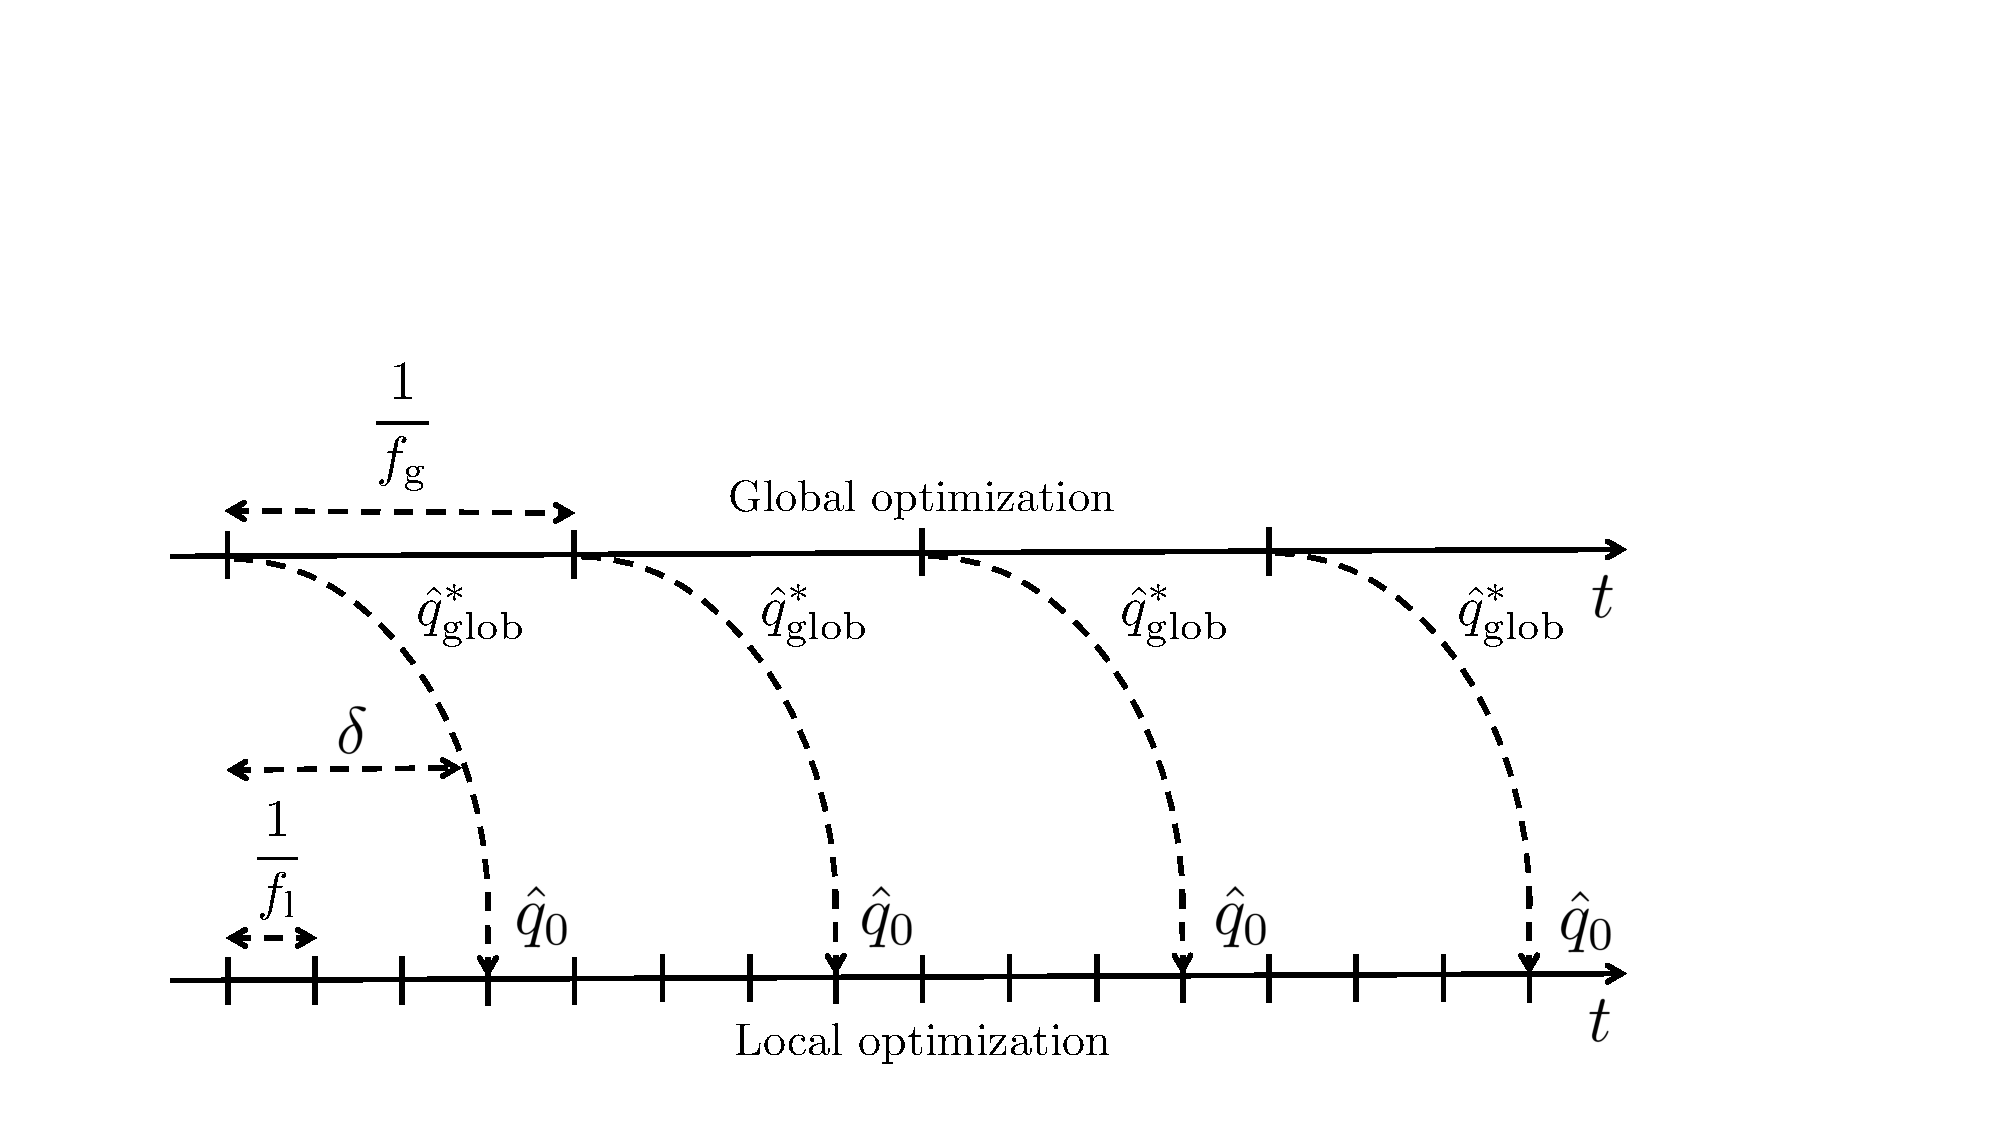
\includegraphics[width=1.0\columnwidth]{promasens/figures/methodology/optimization_scheduling_v2_cropped.pdf}\label{fig:promasens:optimization_scheduling}}\\
    % \subfigure[Local optimization: gradient descent]{\includegraphics[width=1.0\columnwidth]{promasens/figures/methodology/blockdiagram_gradient_descent_v4_cropped.pdf}\label{fig:promasens:blockdiagram_gradient_descent}}
    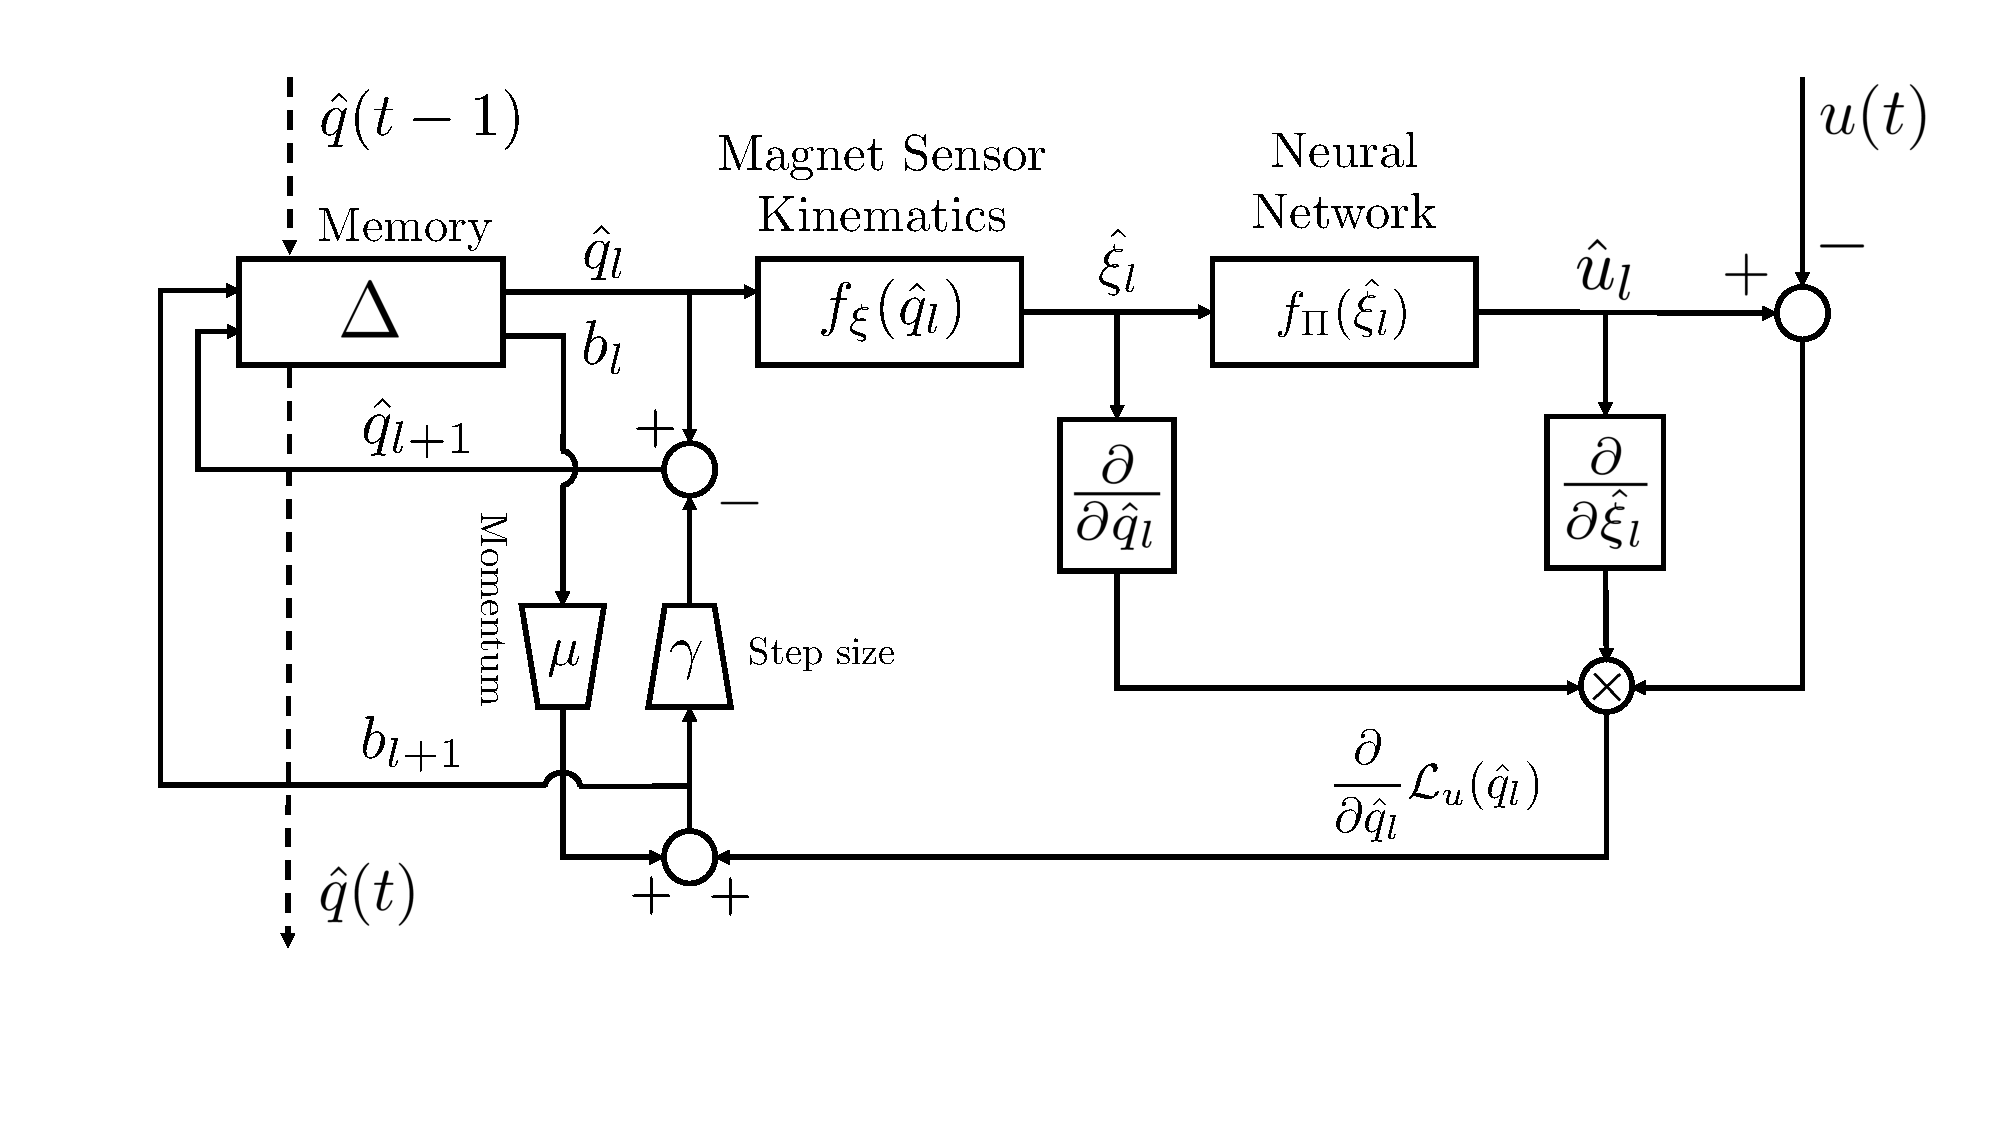
\includegraphics[width=1.0\columnwidth]{promasens/figures/methodology/blockdiagram_gradient_descent_v6_cropped.pdf}
    \caption{% In panel (a), we visualize the scheduling of our chosen optimization strategy: global optimization involving grid search is running at a frequency $f_\mathrm{g}$. In parallel, local gradient descent is performed at a frequency $f_\mathrm{l}$. The global optimization solution arrives $\hat{q}_\mathrm{glob}^*(t-\delta)$ at the local optimization with a delay of $\delta$ and is used to initialize $\hat{q}_0$ for the gradient descent. In all other instances, the gradient descent is initialized with the locally optimized solution $\hat{q}(t-1)$ from the previous time-step. 
    % Panel (b) 
    A block-diagram of the gradient descent as an iterative update loop for the configuration belief $\hat{q}(t)$. The gradient descent is initialized with the optimized solution $\hat{q}_0 = \hat{q}(t-1)$ from the previous time-step. Note that during the iterative loop, $\hat{q}_{l+1}$ updates $\hat{q}_{l}$ in the memory block.}\label{fig:promasens:blockdiagram_gradient_descent}
\end{figure}


\subsection{Data-driven sensor measurement model}
\label{sec:promasens:data_driven_approach}
We use a data-driven approach to learn the forward sensor model $\hat{u} = f_{\pi}(\xi_{j})$ for each sensor using a neural network parameterized with $\pi$.
We note that the same neural network weights can be shared for all sensors, but oftentimes performance can be improved by training a specialized model with weights $\pi_j$ for each sensor.
During training on a dataset of length $n_\mathrm{t}$, we minimize the Mean Squared Error (MSE) error between the predicted sensor measurement $\hat{u}_j$ and the actual sensor measurement $u_j$:
\begin{equation}\small
    \min_{\pi} \frac{1}{n_\mathrm{t}} \sum_{t = 0}^{n_\mathrm{t}} \left ( f_{\pi}(\xi_{j}(t)) - u_j(t) \right )^2,
\end{equation}
where $t$ denotes the current time index.
Note that whenever we omit the time index in our notation, we always refer to the current time $t$.
Finally, to simplify the notation, we combine each sensor measurement prediction $u_j \in \mathbb{R}$ into an array $u \in \mathbb{R}^{n_\mathrm{s}}$ and stack the neural networks as %$u = f_\pi(\xi)$
$f_\Pi(\xi): \xi \rightarrow u$. We discuss the choice of the specific network architecture later in Section~\ref{sec:promasens:pcc_simulations}.

\subsection{Proprioception by optimizing configuration estimate}
\label{sub:promasens:proprioception_optimization}

Now, that we are able to predict the sensor measurement $\hat{u}$ using the composition of the kinematics $f_\xi(\hat{q})$ and the neural networks $f_\Pi(\hat{\xi})$, we need to optimize the configuration estimate $\hat{q}$ for the predictions $\hat{u}$ to match the actual sensor measurements $u$ as closely as possible.
We capture the error between the predicted sensor measurements $\hat{u}$ and the actual sensor measurements $u$ by the MSE loss function we strive to minimize
\begin{equation}\small\label{eq:promasens:proprioception_loss}
    \mathcal{L}_{u}(\hat{q}) = \sum_{j=1}^{n_\mathrm{s}} \frac{\left ( f_\pi(\xi_j) - u_j \right )^2}{n_\mathrm{s}}
\end{equation}
Accordingly, the optimal configuration estimate $\hat{q}$ can be found with
\begin{equation}\small
    \hat{q} = \mathrm{argmin} \: \mathcal{L}_{u}(\hat{q}_l).
\end{equation}

% We employ a dual optimization strategy with global grid search and local gradient descent optimization running in parallel, as visualized in Fig.~\ref{fig:promasens:optimization_scheduling}. As the grid search is computationally expensive, we run it at a frequency of $f_\mathrm{g} \ll f_\mathrm{l}$, where $f_\mathrm{l}$ represents the sampling rate of the gradient descent.
% As we detail in Algorithm~\ref{alg:proprioception}, the gradient descent is nominally initialized with the best estimate of the previous time-step $\hat{q}_0 (t) = \hat{q}(t-1)$.
% When global optimization estimates are available, which are expected to arrive with a computational delay of $\delta$, we use those as an initial condition for the gradient descent.

We optimize the cost function \eqref{eq:promasens:proprioception_loss} through iterative gradient descent, as detailed in Fig.~\ref{fig:promasens:blockdiagram_gradient_descent}. The gradient descent is initialized with the best estimate of the previous time-step $\hat{q}_0 (t) = \hat{q}(t-1)$.
% For the gradient descent itself, detailed in Fig.\ref{fig:promasens:blockdiagram_gradient_descent}, we iteratively
As common in literature, we optimize the state belief $\hat{q}_l$ with a step size $\gamma$ and the momentum $\mu$ using the Jacobian of the loss $\frac{\partial}{\partial \hat{q}_t} \mathcal{L}_{u}(\hat{q})$
\begin{equation}\small\label{eq:promasens:gradient_descent}
    b_{l+1} = \mu \, b_l + \frac{\partial}{\partial \hat{q}_t} \mathcal{L}_{u}(\hat{q}), \quad \hat{q}_{l+1} = \hat{q}_l - \gamma \, b_{l+1}.
\end{equation}
We can use the chain rule to derive an analytical expression for the gradient of the loss incorporating the gradient of the magnet sensor kinematics $\partial_{\hat{q}} f_{\mathrm{\xi}}(\hat{q})$ and the gradient of the neural network $\partial_{\hat{\xi}} f_\Pi (\hat{\xi})$:
\begin{equation}\small
    \frac{\partial}{\partial \hat{q}} \mathcal{L}_{u}(\hat{q}) = \frac{2}{n_\mathrm{s}} \left ( \frac{\partial }{\partial {\hat{q}}} f_{\mathrm{\xi}}(\hat{q}) \right )^\mathrm{T} \, \left ( \frac{\partial}{\partial {\hat{\xi}}} f_\Pi(\hat{\xi}) \right )^\mathrm{T} \, (\hat{u} - u).
\end{equation}
After executing the gradient descent for $n_\mathrm{it}$ iterations, we evaluate which iteration $l^*$ had the lowest loss $\mathcal{L}_{u}$ and accordingly select $\hat{q}(t) = \hat{q}_{l^*}$ as the best configuration estimate of time-step $t$.

\section{Piecewise constant curvature simulations}\label{sec:promasens:pcc_simulations}
We evaluate the proposed methodology for estimating the \gls{PCC} kinematic configuration $q \in \mathbb{R}^{3n_\mathrm{b}}$ of soft continuum robots thoroughly in simulations.
The PCC model allows for bending and elongation of each segment in 3D space. Please refer to Appendix~\ref{sub:promasens:kinematic_model_pcc} for more details.
We vary the number of robot segments $n_\mathrm{b}$, remove and add sensors (i.e. change $n_\mathrm{s}$), modify the arrangement of sensors, and the direction of the earth's magnetic field $n_\mathrm{e}$. 
To motivate some of the unique advantages of our method, we use the same learned neural network weights for all these trials.

\begin{landscape}
\begingroup
\setlength{\tabcolsep}{2pt} % Default value: 6pt
\begin{table*}[hbt]
\centering
\caption{
Simulation results: First, we report the absolute Root Mean-Squared Error (RMSE) $e_{u}$ of sensor measurement predictions on the test set averaged across all sensors on the robot. Next, we state the relative RMSE [\%] of each robot configuration estimate. All results are trained on a trajectory with randomly sampled configurations and sensor kinematic parameters for each segment separately and evaluated on a lemniscate trajectory.
The first section applies our methodology to robots consisting of a different number of segments $n_\mathrm{b}$ with three sensors attached to the tip of each segment.
The number of sensors is varied in the second section for a three-segment robot with all sensors placed symmetrically. 
The third set of trials then investigates how robust the method is to change the kinematic parameters of the sensors, such as the tilting angle of the sensors $\psi_\mathrm{s}$ and the radial distance of the sensors $d_{\mathrm{s},\mathrm{r}}$.
Finally, we apply the earth's magnetic field along different cardinal directions in the inertial frame.
The RMSE of the configuration estimates is normalized with the range of the dataset for each configuration variable as stated in \eqref{eq:promasens:relative_RMSE}. We report the error as $\text{mean} \pm \text{stdev}$ and compute the statistics over three different random seeds. The random seed determines at the start of the training the initialization of the neural network weights.
}
% \begin{tabular}{l r rrr rrr rrr}\toprule
% \textbf{Simulation} & $e_{u}$ [mT] & $e_{\Delta_{x,1}}$ [\%] & $e_{\Delta_{y,1}}$ [\%] & $e_{\delta L_1}$ [\%] & $e_{\Delta_{x,2}}$ [\%] & $e_{\Delta_{y,2}}$ [\%] & $e_{\delta L_2}$ [\%] & $e_{\Delta_{x,3}}$ [\%] & $e_{\Delta_{y,3}}$ [\%] & $e_{\delta L_3}$ [\%]\\
% \midrule
% \# of segments: $n_\mathrm{b} = 1$ & $1.5 \pm 0.2$ & $1.7 \pm 1.0$ & $1.8 \pm 1.1$ & $2.8 \pm 0.6$ & - & - & - & - & - & -\\
% \# of segments: $n_\mathrm{b} = 2$ & $1.5 \pm 0.1$ & $4.2 \pm 1.3$ & $3.9 \pm 0.6$ & $6.3 \pm 1.3$ & $2.3 \pm 0.6$ & $2.2 \pm 0.3$ & $4.1 \pm 1.3$ & - & - & -\\
% \# of segments: $n_\mathrm{b} = 3$ & $1.5 \pm 0.2$ & $3.7 \pm 2.1$ & $4.7 \pm 1.6$ & $6.0 \pm 2.0$ & $2.6 \pm 1.6$ & $2.5 \pm 1.5$ & $5.5 \pm 1.6$ & $1.6 \pm 1.2$ & $1.6 \pm 1.1$ & $2.7 \pm 1.4$\\
% \midrule
% \# of sensors: $n_\mathrm{s} = 6$ & $1.5 \pm 0.2$ & $3.9 \pm 1.2$ & $24.4 \pm 2.7$ & $8.4 \pm 2.6$ & $2.5 \pm 1.3$ & $53.2 \pm 5.0$ & $6.0 \pm 1.7$ & $1.5 \pm 1.1$ & $52.3 \pm 7.3$ & $3.1 \pm 1.0$\\
% \# of sensors: $n_\mathrm{s} = 9$ & $1.5 \pm 0.2$ & $3.7 \pm 2.1$ & $4.7 \pm 1.6$ & $6.0 \pm 2.0$ & $2.6 \pm 1.6$ & $2.5 \pm 1.5$ & $5.5 \pm 1.6$ & $1.6 \pm 1.2$ & $1.6 \pm 1.1$ & $2.7 \pm 1.4$\\
% \# of sensors: $n_\mathrm{s} = 12$ & $1.5 \pm 0.1$ & $3.7 \pm 1.6$ & $3.9 \pm 1.3$ & $4.6 \pm 2.4$ & $2.6 \pm 1.3$ & $2.6 \pm 1.2$ & $4.4 \pm 1.9$ & $1.6 \pm 1.2$ & $1.5 \pm 1.3$ & $2.5 \pm 1.6$\\
% \# of sensors: $n_\mathrm{s} = 18$ & $1.6 \pm 0.2$ & $3.2 \pm 1.5$ & $3.5 \pm 1.3$ & $4.2 \pm 1.8$ & $2.4 \pm 1.3$ & $2.5 \pm 1.2$ & $4.4 \pm 1.8$ & $1.5 \pm 1.3$ & $1.3 \pm 1.1$ & $2.5 \pm 1.5$\\
% \midrule
% nominal & $1.5 \pm 0.2$ & $3.7 \pm 2.1$ & $4.7 \pm 1.6$ & $6.0 \pm 2.0$ & $2.6 \pm 1.6$ & $2.5 \pm 1.5$ & $5.5 \pm 1.6$ & $1.6 \pm 1.2$ & $1.6 \pm 1.1$ & $2.7 \pm 1.4$\\
% sensors tilted: $\psi_\mathrm{s} = \SI{10}{\degree}$ & $1.5 \pm 0.2$ & $8.1 \pm 4.0$ & $6.4 \pm 2.0$ & $4.7 \pm 0.7$ & $5.1 \pm 2.3$ & $3.8 \pm 0.8$ & $5.6 \pm 2.4$ & $2.8 \pm 1.2$ & $1.9 \pm 0.8$ & $4.1 \pm 0.6$\\
% $d_{\mathrm{s},\mathrm{r}} = \SI{16}{mm}, \psi_\mathrm{s} = \SI{10}{\degree}$ & $1.5 \pm 0.1$ & $4.0 \pm 2.1$ & $4.3 \pm 1.6$ & $4.6 \pm 1.3$ & $2.9 \pm 0.3$ & $2.4 \pm 0.3$ & $5.2 \pm 1.6$ & $1.6 \pm 1.0$ & $1.6 \pm 0.8$ & $3.1 \pm 1.0$ \\
% % \midrule
% % FEM nominal & $0.0 \pm 0.0$ & $0.0 \pm 0.0$ & $0.0 \pm 0.0$ & $0.0 \pm 0.0$ & $0.0 \pm 0.0$ & $0.0 \pm 0.0$ & $0.0 \pm 0.0$ & $0.0 \pm 0.0$ & $0.0 \pm 0.0$ & $0.0 \pm 0.0$\\
% \bottomrule
% \end{tabular}

\begin{tabular}{cl r rrr rrr rrr}\toprule
\textbf{Simulation} & \textbf{Specifications} & $e_{u}$ [mT] & $e_{\Delta_{x,1}}$ [\%] & $e_{\Delta_{y,1}}$ [\%] & $e_{\delta L_1}$ [\%] & $e_{\Delta_{x,2}}$ [\%] & $e_{\Delta_{y,2}}$ [\%] & $e_{\delta L_2}$ [\%] & $e_{\Delta_{x,3}}$ [\%] & $e_{\Delta_{y,3}}$ [\%] & $e_{\delta L_3}$ [\%]\\
\midrule
\multirow{3}{*}{\makecell{Variation of\\ \# of segments}} & $n_\mathrm{b}$=1, $n_\mathrm{s}$=3 & $0.015 \pm 0.002$ & $1.7 \pm 1.0$ & $1.8 \pm 1.1$ & $2.8 \pm 0.6$ & - & - & - & - & - & -\\
& $n_\mathrm{b}$=2, $n_\mathrm{s}$=6 & $0.015 \pm 0.001$ & $4.2 \pm 1.3$ & $3.9 \pm 0.6$ & $6.3 \pm 1.3$ & $2.3 \pm 0.6$ & $2.2 \pm 0.3$ & $4.1 \pm 1.3$ & - & - & -\\
& $n_\mathrm{b}$=3, $n_\mathrm{s}$=9 & $0.015 \pm 0.002$ & $3.7 \pm 2.1$ & $4.7 \pm 1.6$ & $6.0 \pm 2.0$ & $2.6 \pm 1.6$ & $2.5 \pm 1.5$ & $5.5 \pm 1.6$ & $1.6 \pm 1.2$ & $1.6 \pm 1.1$ & $2.7 \pm 1.4$\\
\midrule
\multirow{4}{*}{\makecell{Variation of\\ \# of sensors}} &$n_\mathrm{b}$=3, $n_\mathrm{s}$=6 & $0.015 \pm 0.002$ & $3.9 \pm 1.2$ & $24.4 \pm 2.7$ & $8.4 \pm 2.6$ & $2.5 \pm 1.3$ & $53.2 \pm 5.0$ & $6.0 \pm 1.7$ & $1.5 \pm 1.1$ & $52.3 \pm 7.3$ & $3.1 \pm 1.0$\\
&$n_\mathrm{b}$=3, $n_\mathrm{s}$=9 & $0.015 \pm 0.002$ & $3.7 \pm 2.1$ & $4.7 \pm 1.6$ & $6.0 \pm 2.0$ & $2.6 \pm 1.6$ & $2.5 \pm 1.5$ & $5.5 \pm 1.6$ & $1.6 \pm 1.2$ & $1.6 \pm 1.1$ & $2.7 \pm 1.4$\\
&$n_\mathrm{b}$=3, $n_\mathrm{s}$=12 & $0.015 \pm 0.001$ & $3.7 \pm 1.6$ & $3.9 \pm 1.3$ & $4.6 \pm 2.4$ & $2.6 \pm 1.3$ & $2.6 \pm 1.2$ & $4.4 \pm 1.9$ & $1.6 \pm 1.2$ & $1.5 \pm 1.3$ & $2.5 \pm 1.6$\\
&$n_\mathrm{b}$=3, $n_\mathrm{s}$=18 & $0.016 \pm 0.002$ & $3.2 \pm 1.5$ & $3.5 \pm 1.3$ & $4.2 \pm 1.8$ & $2.4 \pm 1.3$ & $2.5 \pm 1.2$ & $4.4 \pm 1.8$ & $1.5 \pm 1.3$ & $1.3 \pm 1.1$ & $2.5 \pm 1.5$\\
\midrule
Nominal & $n_\mathrm{b}$=3, $n_\mathrm{s}$= 9 & $0.015 \pm 0.002$ & $3.7 \pm 2.1$ & $4.7 \pm 1.6$ & $6.0 \pm 2.0$ & $2.6 \pm 1.6$ & $2.5 \pm 1.5$ & $5.5 \pm 1.6$ & $1.6 \pm 1.2$ & $1.6 \pm 1.1$ & $2.7 \pm 1.4$\\
Sensors tilted & $\psi_\mathrm{s}$=\SI{10}{\degree} & $0.015 \pm 0.002$ & $8.1 \pm 4.0$ & $6.4 \pm 2.0$ & $4.7 \pm 0.7$ & $5.1 \pm 2.3$ & $3.8 \pm 0.8$ & $5.6 \pm 2.4$ & $2.8 \pm 1.2$ & $1.9 \pm 0.8$ & $4.1 \pm 0.6$\\
Sensors shifted & $d_{\mathrm{s},\mathrm{r}}$=\SI{16}{mm} & $0.017 \pm 0.003$ & $3.4 \pm 1.5$ & $4.0 \pm 1.3$ & $6.2 \pm 2.5$ & $2.6 \pm 1.0$ & $2.8 \pm 1.8$ & $6.7 \pm 0.9$ & $1.6 \pm 1.2$ & $1.6 \pm 1.0$ & $4.0 \pm 2.0$ \\
\midrule
\multirow{3}{*}{\makecell{Earth\\ magnetic\\ field}} & $n_\mathrm{e}$=$(1,0,0)$ & $0.012 \pm 0.002$ & $2.0 \pm 0.4$ & $2.4 \pm 1.1$ & $4.3 \pm 1.3$ & $1.8 \pm 0.7$ & $1.9 \pm 0.3$ & $3.6 \pm 2.0$ & $1.5 \pm 0.3$ & $1.6 \pm 0.4$ & $3.2 \pm 0.9$\\
& $n_\mathrm{e}$=$(0,1,0)$ & $0.012 \pm 0.002$ & $1.9 \pm 0.5$ & $2.5 \pm 0.8$ & $3.8 \pm 1.1$ & $1.9 \pm 0.5$ & $2.0 \pm 0.2$ & $3.4 \pm 1.6$ & $1.5 \pm 0.3$ & $1.6 \pm 0.4$ & $3.3 \pm 0.8$\\
& $n_\mathrm{e}$=$(0,0,1)$ & $0.012 \pm 0.001$ & $2.0 \pm 0.7$ & $2.6 \pm 0.9$ & $4.1 \pm 0.9$ & $1.6 \pm 0.3$ & $1.7 \pm 0.3$ & $4.9 \pm 1.5$ & $1.5 \pm 0.5$ & $1.4 \pm 0.1$ & $3.9 \pm 0.3$\\
% \midrule
% FEM nominal & $0.0 \pm 0.0$ & $0.0 \pm 0.0$ & $0.0 \pm 0.0$ & $0.0 \pm 0.0$ & $0.0 \pm 0.0$ & $0.0 \pm 0.0$ & $0.0 \pm 0.0$ & $0.0 \pm 0.0$ & $0.0 \pm 0.0$ & $0.0 \pm 0.0$\\
\bottomrule
\end{tabular}
\label{tab:results_pcc_simulations}
\end{table*}
\endgroup
\end{landscape}

\begin{figure*}[hbt]
\centering
    \subfigure[Magnetic field for a three-segment robot]{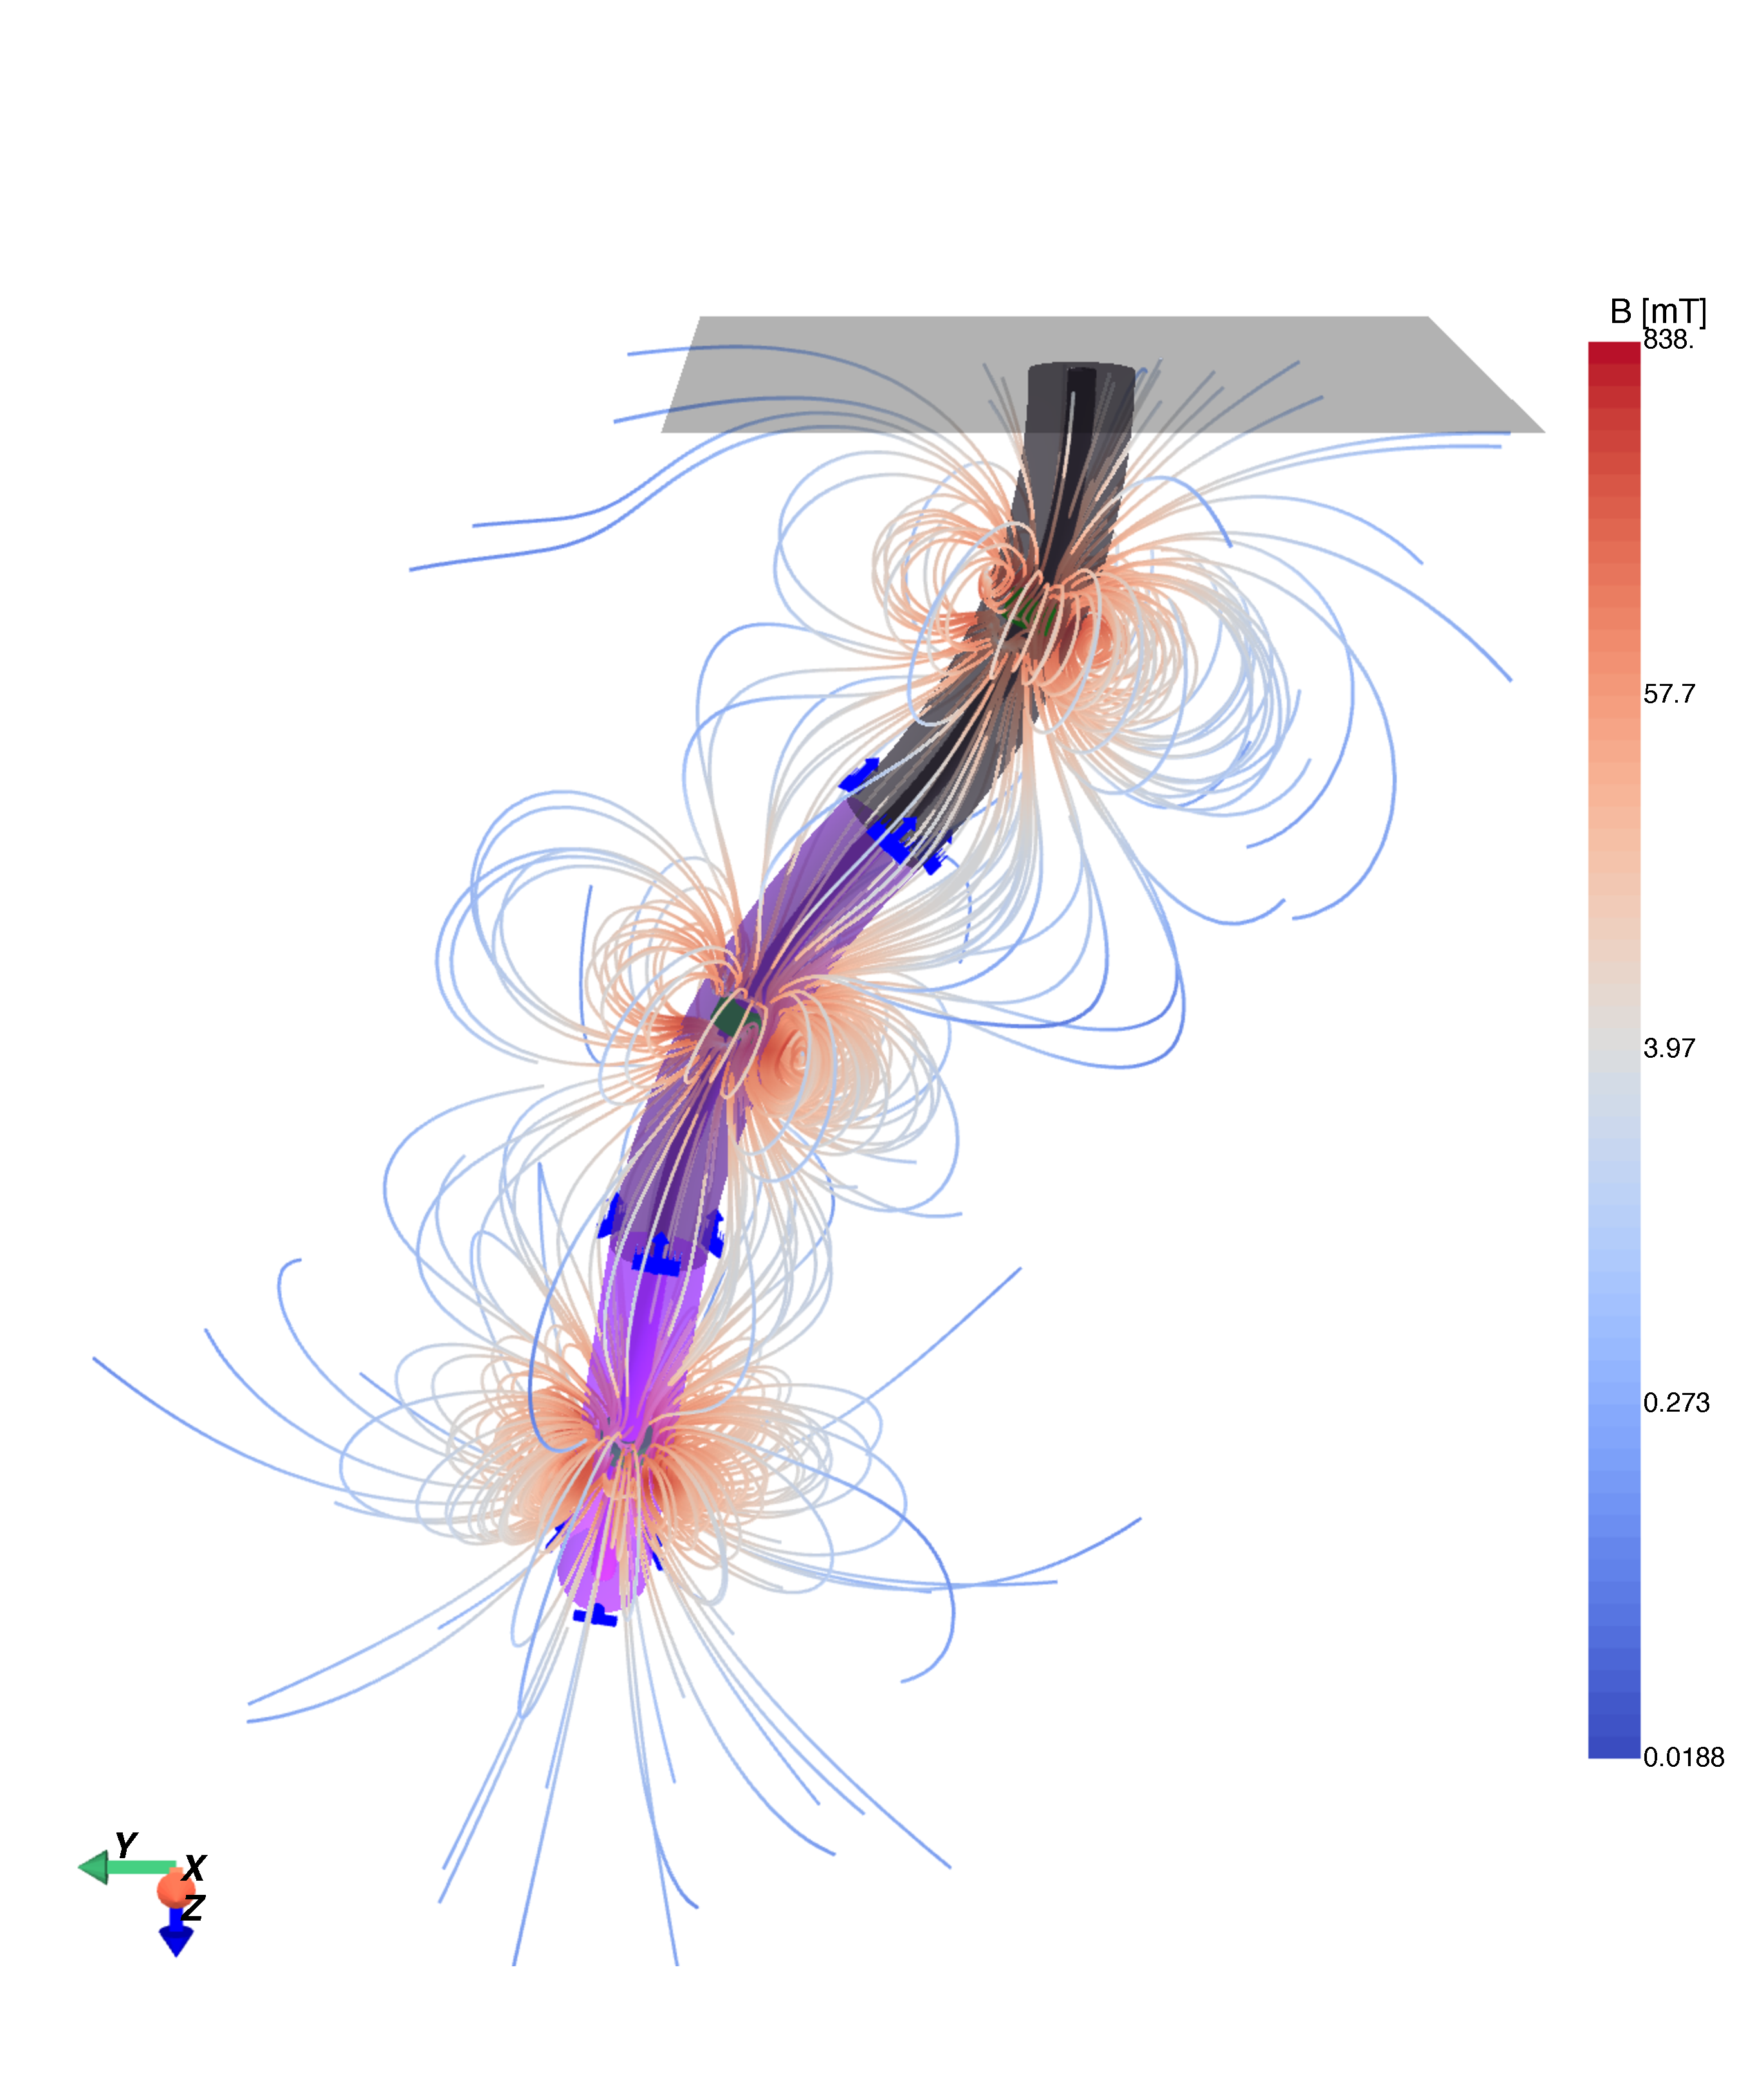
\includegraphics[width=0.3\textwidth]{promasens/figures/simulation_setup/analytical_simulation_three_segment_v2_cropped.pdf}}
    \subfigure[Simulated sensor failure]{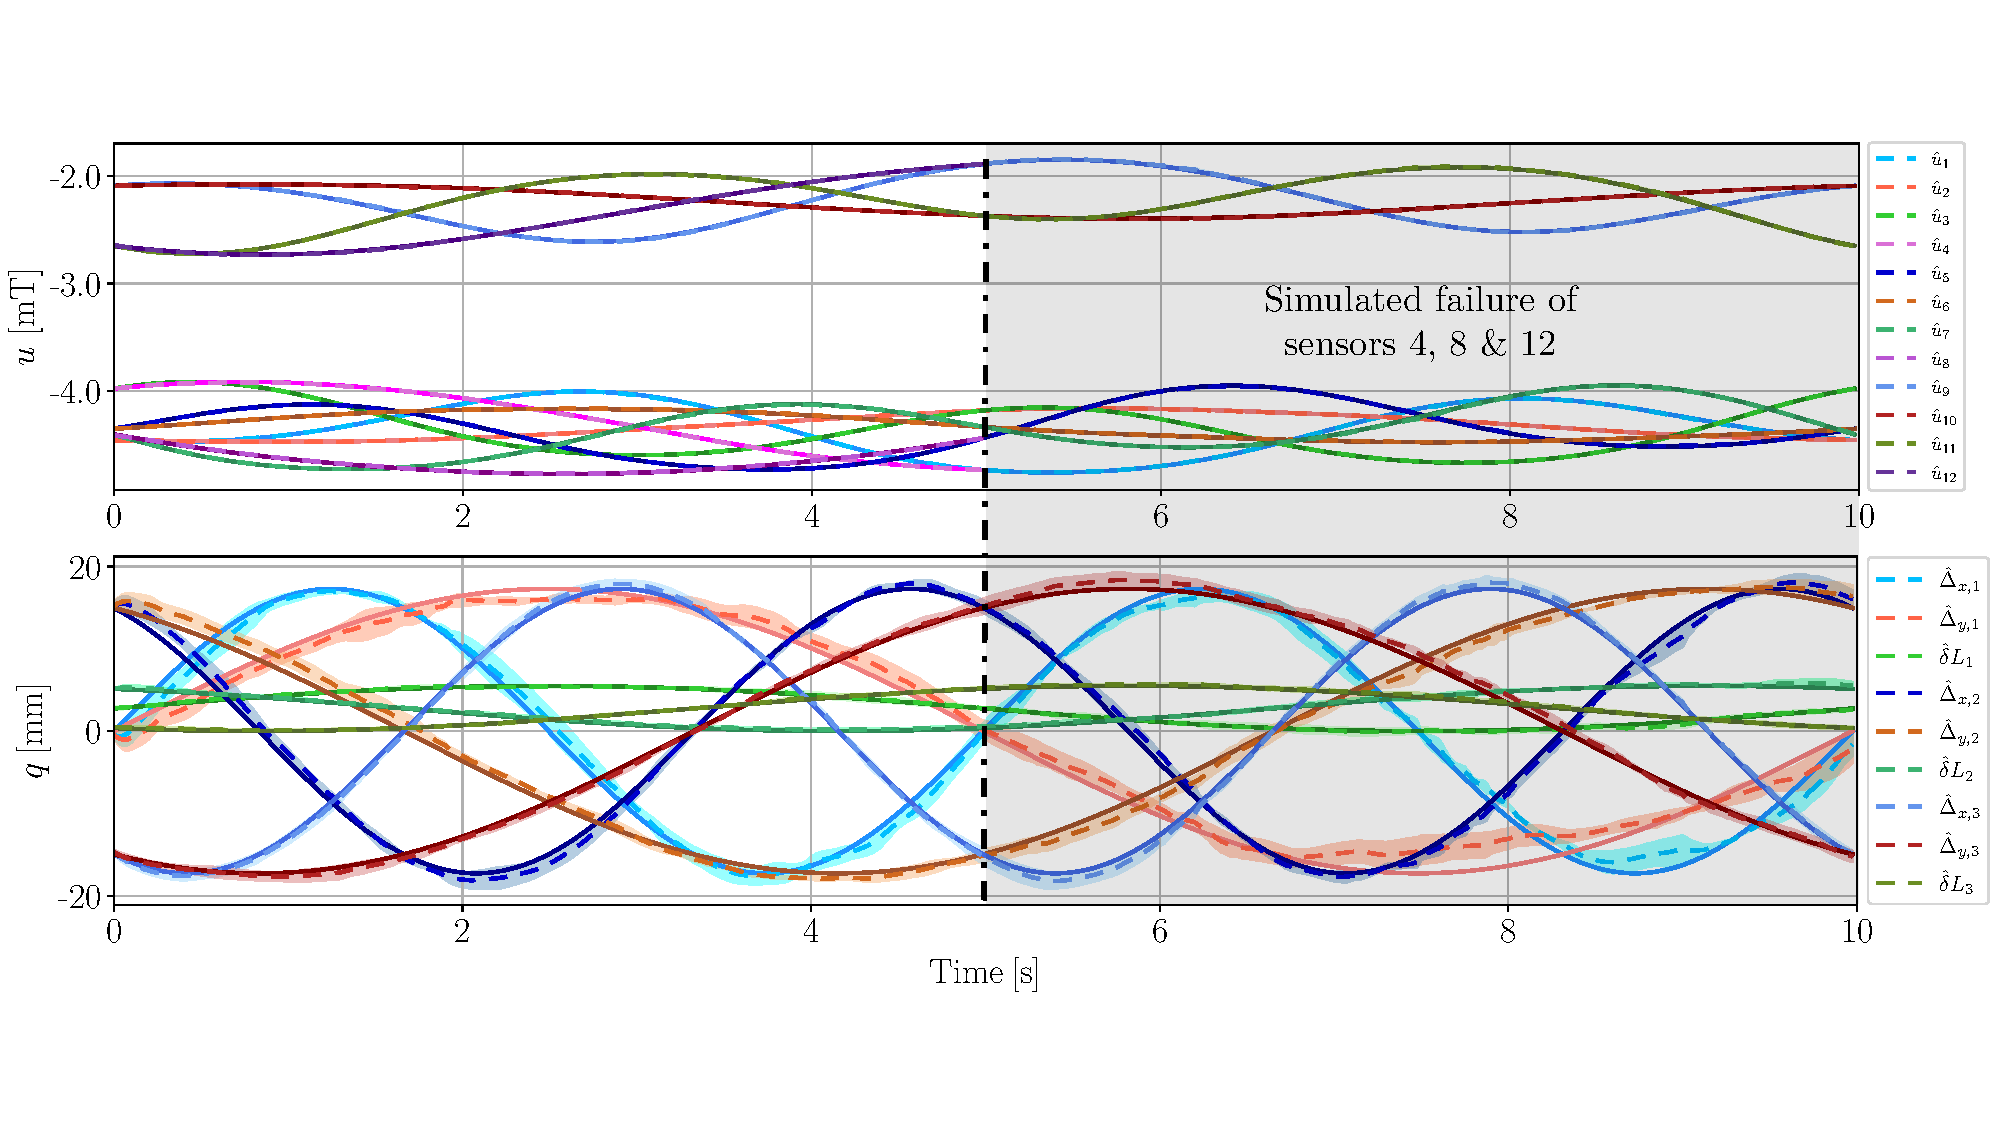
\includegraphics[width=0.68\textwidth]{promasens/figures/simulation_results/pcc/simulated_sensor_failure_cropped.pdf}\label{fig:promasens:simulated_sensor_failure}}
\caption{\textbf{Panel (a):} Simulated magnetic field of a robot with three segments. The blue arrows mark the measurement directions of the sensors, the magnets are rendered in green and the three segments are visualized in a color sequence from black to violet. The magnetic flux density $B$ is shown via streamlines and logarithmic coloring. \textbf{Panel (b)}: Sensor measurement predictions (top) and configuration estimates (bottom) for a three-segment robot with twelve sensors nominally. We simulate a sensor failure of the 4th, 8th, and 12th sensors after \SI{5}{s} of trajectory time by removing the measurements of these sensors from the gradient descent. This can be compensated automatically by the redundancy of the sensor configuration. We plot the ground-truth values $u$ and $q$ in solid, the estimate $\hat{u}$ and $\hat{q}$ as a mean over three random seeds with dashed lines and the standard deviation as an error band.}
\end{figure*}

\subsection{Simulation setup}\label{sub:promasens:pcc_simulations:simulation_setup}
In our simulations, we consider a robot consisting of one, two, or three segments. % which all behave according to the Constant Curvature (CC) assumption and can also elongate~\cite{della2020improved}. 
All cylindrical segments have an unextended length of $L_{0,i} = \SI{110}{mm}$ and a radius of $d_i = \SI{22}{mm}$. Each segment has a neodymium N50 ring magnet of outer diameter \SI{12}{mm}, inner diameter \SI{6}{mm} and thickness \SI{6}{mm} integrated along the backbone at a distance of $d_{\mathrm{m}_k} = \SI{55}{mm}$ from the base of the segment.
In the nominal case, three sensors are placed symmetrically in the tip plane of each segment at a radius of \SI{13}{mm} from the center with the sensor measurement direction pointing along the local, negative z-axis of the tip plane $\{S_i\}$. We also consider alternative placements of the sensors, which we further detail in Section~\ref{sub:promasens:simulation_pcc_results}.

% \subsection{Magnetic field simulation}
% The crucial component of our simulation is the prediction of the magnetic field and corresponding sensor measurements for a given pose of the magnets.
% For this, we leverage Magpylib~\cite{magpylib2020}, a Python package for computing 3D static magnetic fields using analytical solutions.
We build on Magpylib~\cite{magpylib2020} to simulate the magnetic field behavior.
We model the magnets as cylindrical neodymium grade N50 rings with a magnetization of \SI{1450}{mT} in the local z-direction. 
After simulating the magnetic field, we rotate the B-field into the local reference frame of each sensor and take the local z-component of the magnetic flux density as the sensor measurement.
%Additionally, we add a static B-field representing the earth's magnetic field influence along the inertial x-axis and a magnitude of \SI{65}{\micro T}. To simulate the sensor measurements, we take into account the component of the B-field pointing along the local z-axis of the sensor.

% \subsection{Magnetic field simulation \textcolor{orange}{FEM}}
% We build on Netgen / NGSolve~\cite{netgen_ngsolve} to simulate the magnetic field behavior using \gls{FEM} by implementing the magnetostatic Maxwell equations.
% We model a cylindrical Neodymium grade N50 ring magnet with a magnetization of $M=(0,0,\SI{1.45}{T})^\mathrm{T}$ in local z-direction and a relative permeability of $\mu_r = 1.05$. 
% % Additionally, we add a static B-field representing the earth's magnetic field influence along the inertial x-axis and a magnitude of \SI{65}{\micro T}. To simulate the sensor measurements, we take into account the component of the B-field pointing along the local z-axis of the sensor.
% The remaining part of the control volume
% We mesh the magnets and the air with a maximum mesh size of \SI{6}{mm} and \SI{220}{mm} respectively.
% After solving the finite element problem, we rotate the B-field into the local reference frame for each sensor and take the z-component of the magnetic flux density as the sensor measurement.
%

\subsection{Prediction network}\label{sub:promasens:pcc_simulations:neural_network}
The training set consists of \SI{120000}{} random configurations sampled from uniform distribution $\Delta_{x,i} \sim \mathcal{U}(-\SI{20.7}{mm}, \SI{20.7}{mm})$, $\Delta_{y,i} \sim \mathcal{U}(-\SI{20.7}{mm}, \SI{20.7}{mm})$, and $\delta L_i \sim \mathcal{U}(0, \SI{5.5}{mm})$, where the upper bound represents a bending of the tip of \SI{54}{\degree} with respect to the base of a segment and an elongation of \SI{5}{\percent}. We also randomize the placement of the sensors in the training set. While in the nominal case, the first of the symmetrically placed sensors is placed on the local x-axis, we randomly sample an offset angle $\varphi_\mathrm{off} \sim \mathcal{U}(0, \frac{2\pi}{n_{\mathrm{s}_i}})$ for each training sample, where $n_{\mathrm{s}_i} = 3$ is the number of sensors per segment.
Finally, we also randomly sample the radial displacement of the sensors from the center with $d_{\mathrm{s}, \mathrm{r}} \sim \mathcal{U}(8.7, 17.3) \mathrm{mm}$ and consider a tilting of the sensors (e.g. a rotation around the tangential axis) with $\psi_\mathrm{s} \sim \mathcal{U}(\SI{-20}{\degree}, \SI{20}{\degree})$.
Before training, we randomly split off \SI{30}{\percent} of the training set for validation purposes.

We conducted a selection study involving hyperparameters and feed-forward neural network architectures (number of layers, nodes, and nonlinear activation layer types) on the validation set. % to select our training procedure for the sensor measurement prediction network. 
In particular, we aimed to generate a smooth loss landscape to improve the gradient descent convergence leading us to employ a Stochastic Gradient Descent (SGD) % ~\cite{ruder2016overview} 
optimizer in conjunction with the Stochastic Weight Averaging (SWA)~\cite{izmailov2018averaging} strategy.
The neural network itself %as depicted in Figure~\ref{fig:promasens:NNgradientdescent}
has $18$ layers in total and contains, after an initial 1D batch norm layer, four blocks and is concluded with a fully-connected layer at the end. Each block consists of a dropout with a probability of \SI{1}{\percent}, a linear layer, a ReLU, and a 1D batch norm layer. The hidden state is first increased to $96$ nodes, then to $256$ nodes, and finally reduced again to $64$ and $24$ nodes.
We minimize a Mean Squared Error (MSE) loss of the neural network prediction $\hat{u}_j(t)$ for $250$ epochs with batch size $650$ while setting an initial learning rate of $0.18$ for the cosine annealing learning rate scheduler~\cite{loshchilov2016sgdr}. The SWA~\cite{izmailov2018averaging} strategy is started after $125$ epochs.
% We train a neural network $f_{\pi_i}(\xi_j)$ for all sensors in each segment $i$.
We train the neural network such that all sensors in the $i^\mathrm{th}$ segment share the same weights $\pi_i$.
% The reason for this is that the sensors in the distal segment measure much lower magnetic field magnitudes than the sensors in the other segments as they are only influenced by one magnet (e.g. the magnet in the distal segment) resulting in poor convergence behavior when trained jointly on all segments.
When the training is finished, we select the model from the epoch with the lowest validation loss and save it for later testing.

\begin{figure*}[hbt]
  \centering
  \subfigure[$t=\SI{0}{s}$]{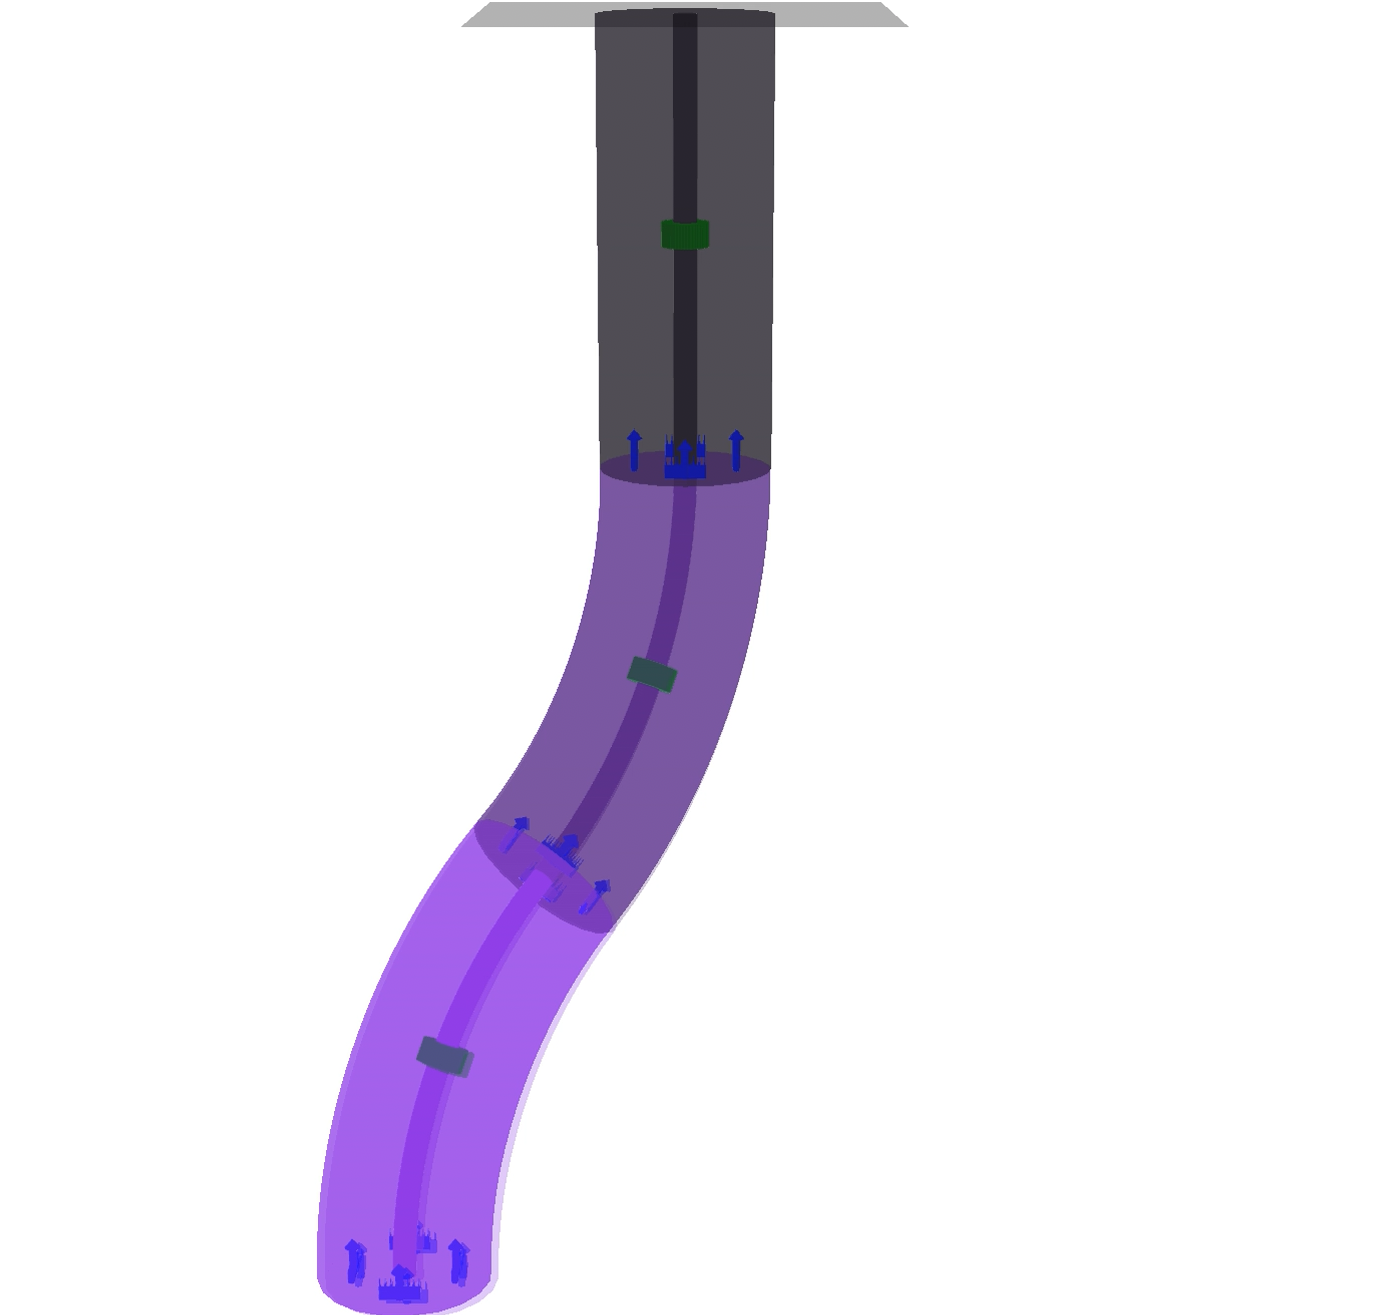
\includegraphics[width=0.161\textwidth]{promasens/figures/simulation_sequences/pcc_simulated_sensor_failure/simulated_sensor_failure_t=0s_cropped.png}}
  \hfill
  \subfigure[$t=\SI{2}{s}$]{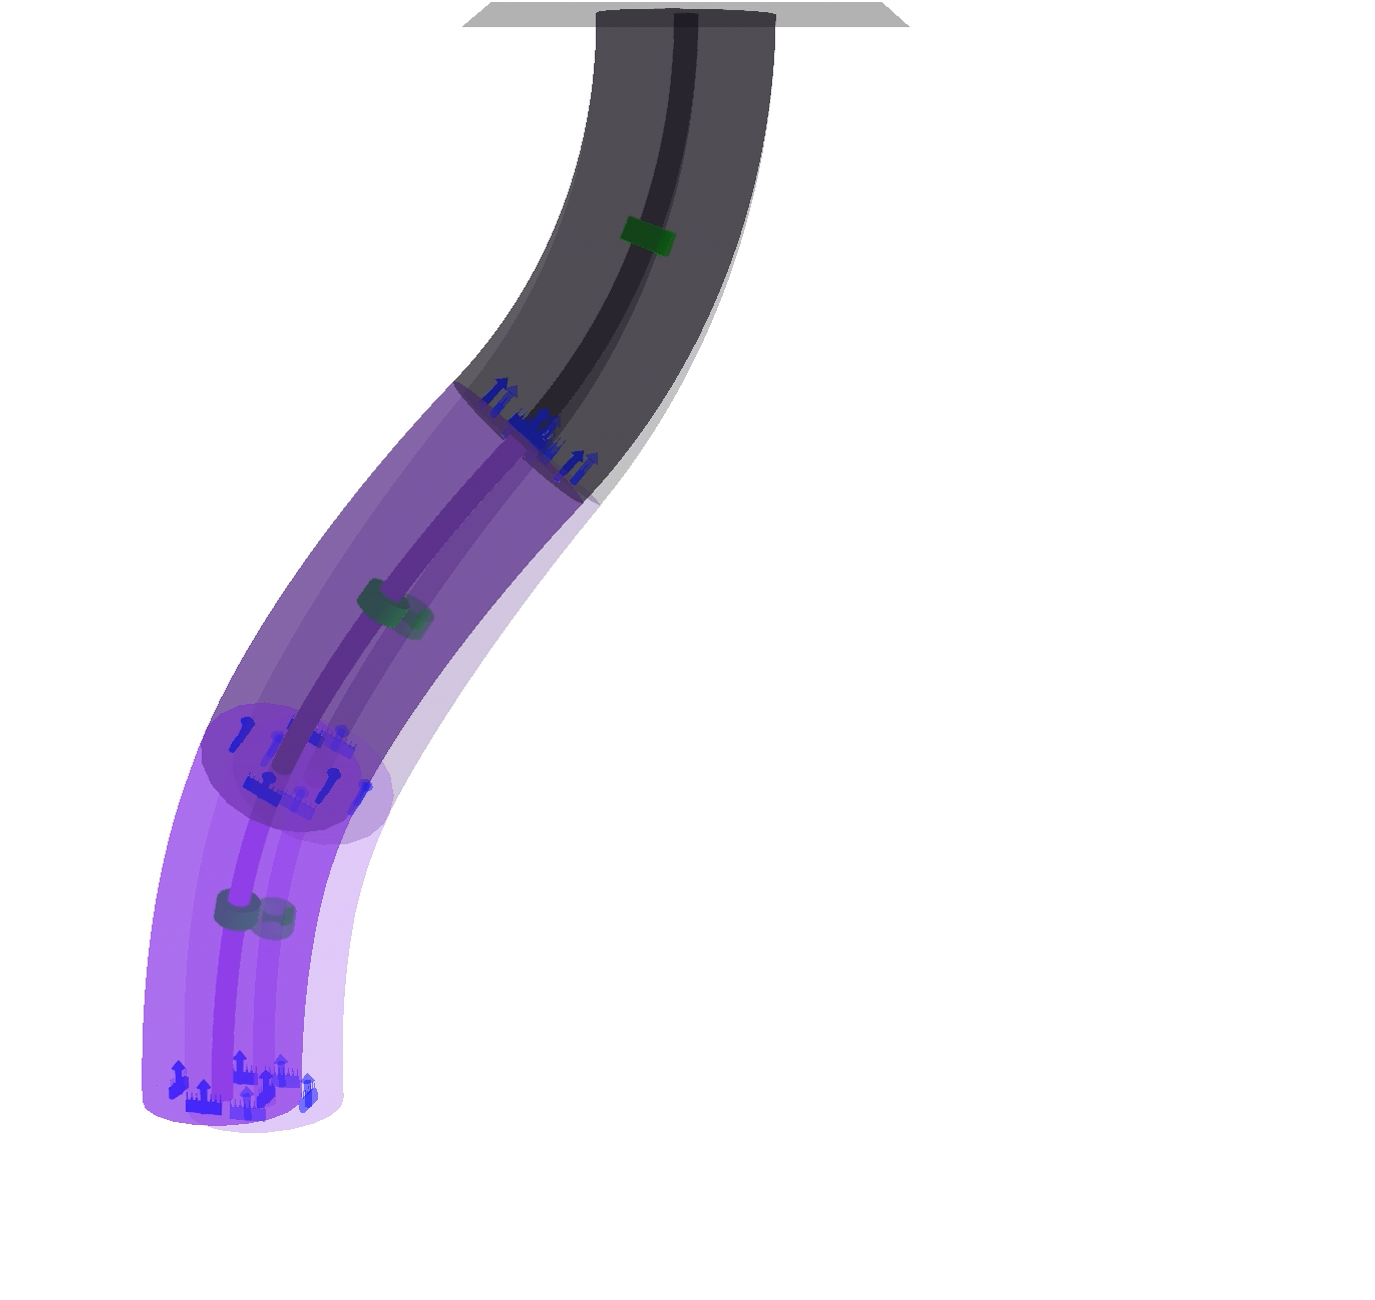
\includegraphics[width=0.161\textwidth]{promasens/figures/simulation_sequences/pcc_simulated_sensor_failure/simulated_sensor_failure_t=2s_cropped.png}}
  \hfill
  \subfigure[$t=\SI{4}{s}$]{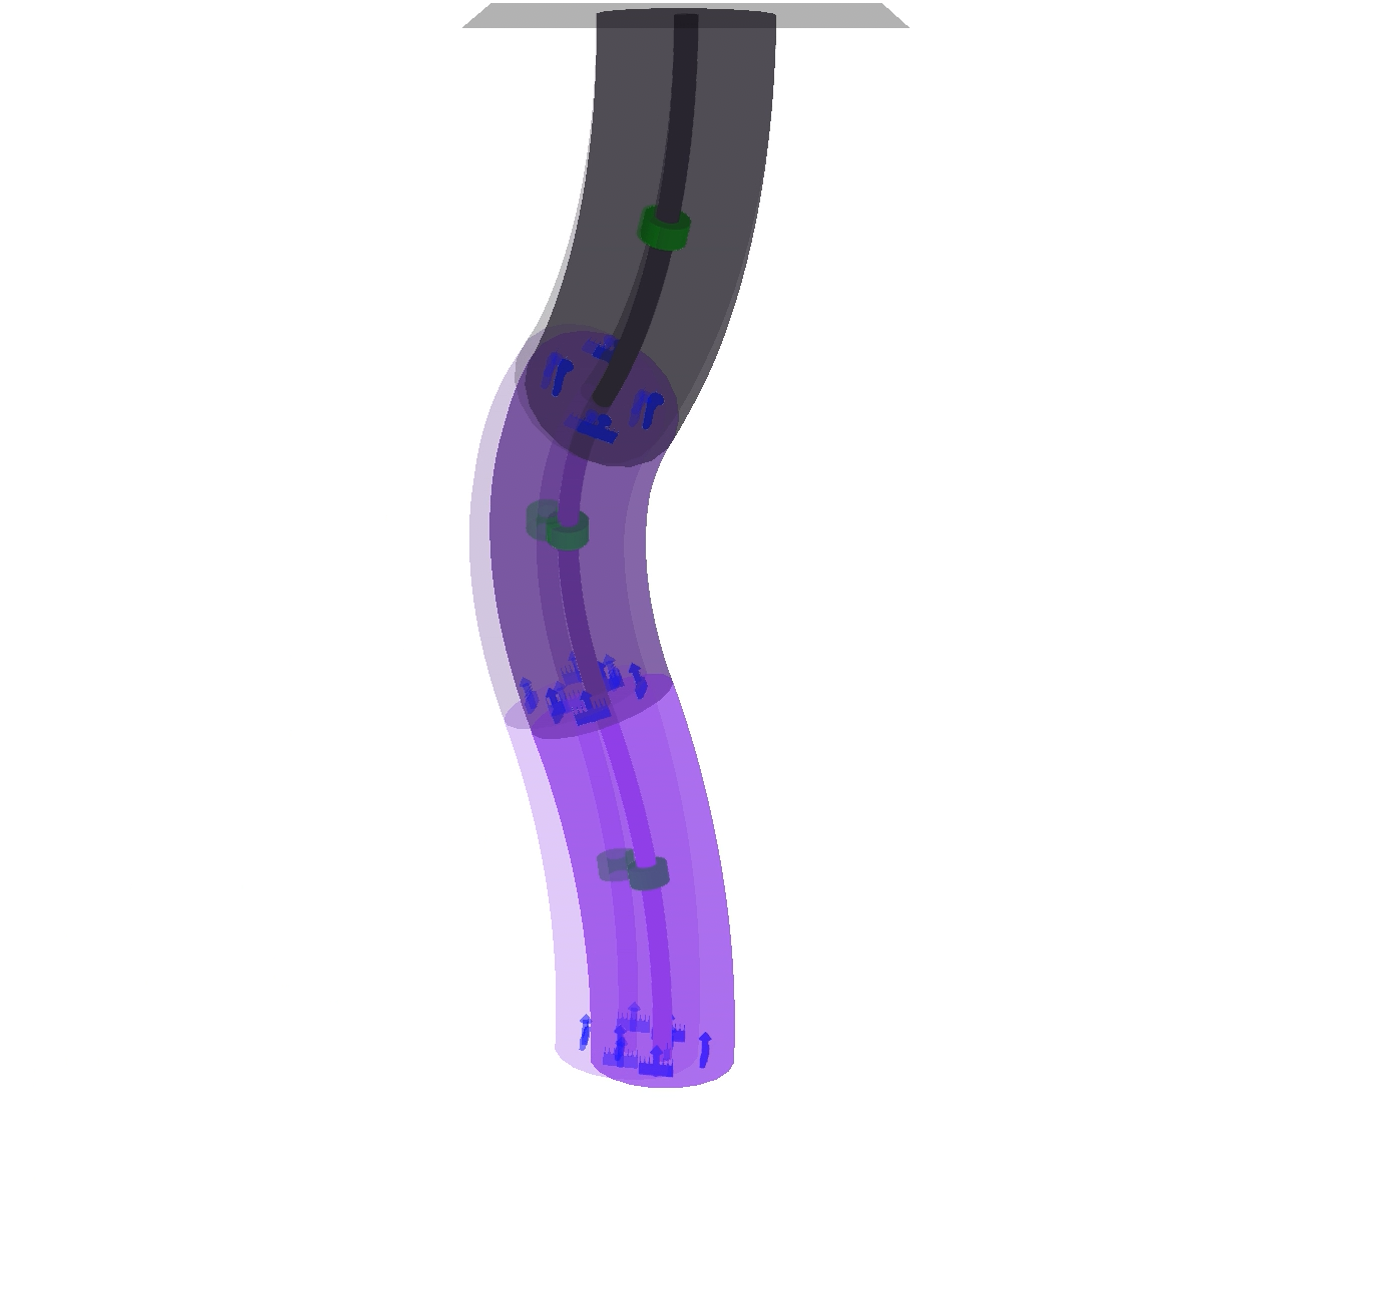
\includegraphics[width=0.161\textwidth]{promasens/figures/simulation_sequences/pcc_simulated_sensor_failure/simulated_sensor_failure_t=4s_cropped.png}}
  \hfill
  \subfigure[$t=\SI{6}{s}$]{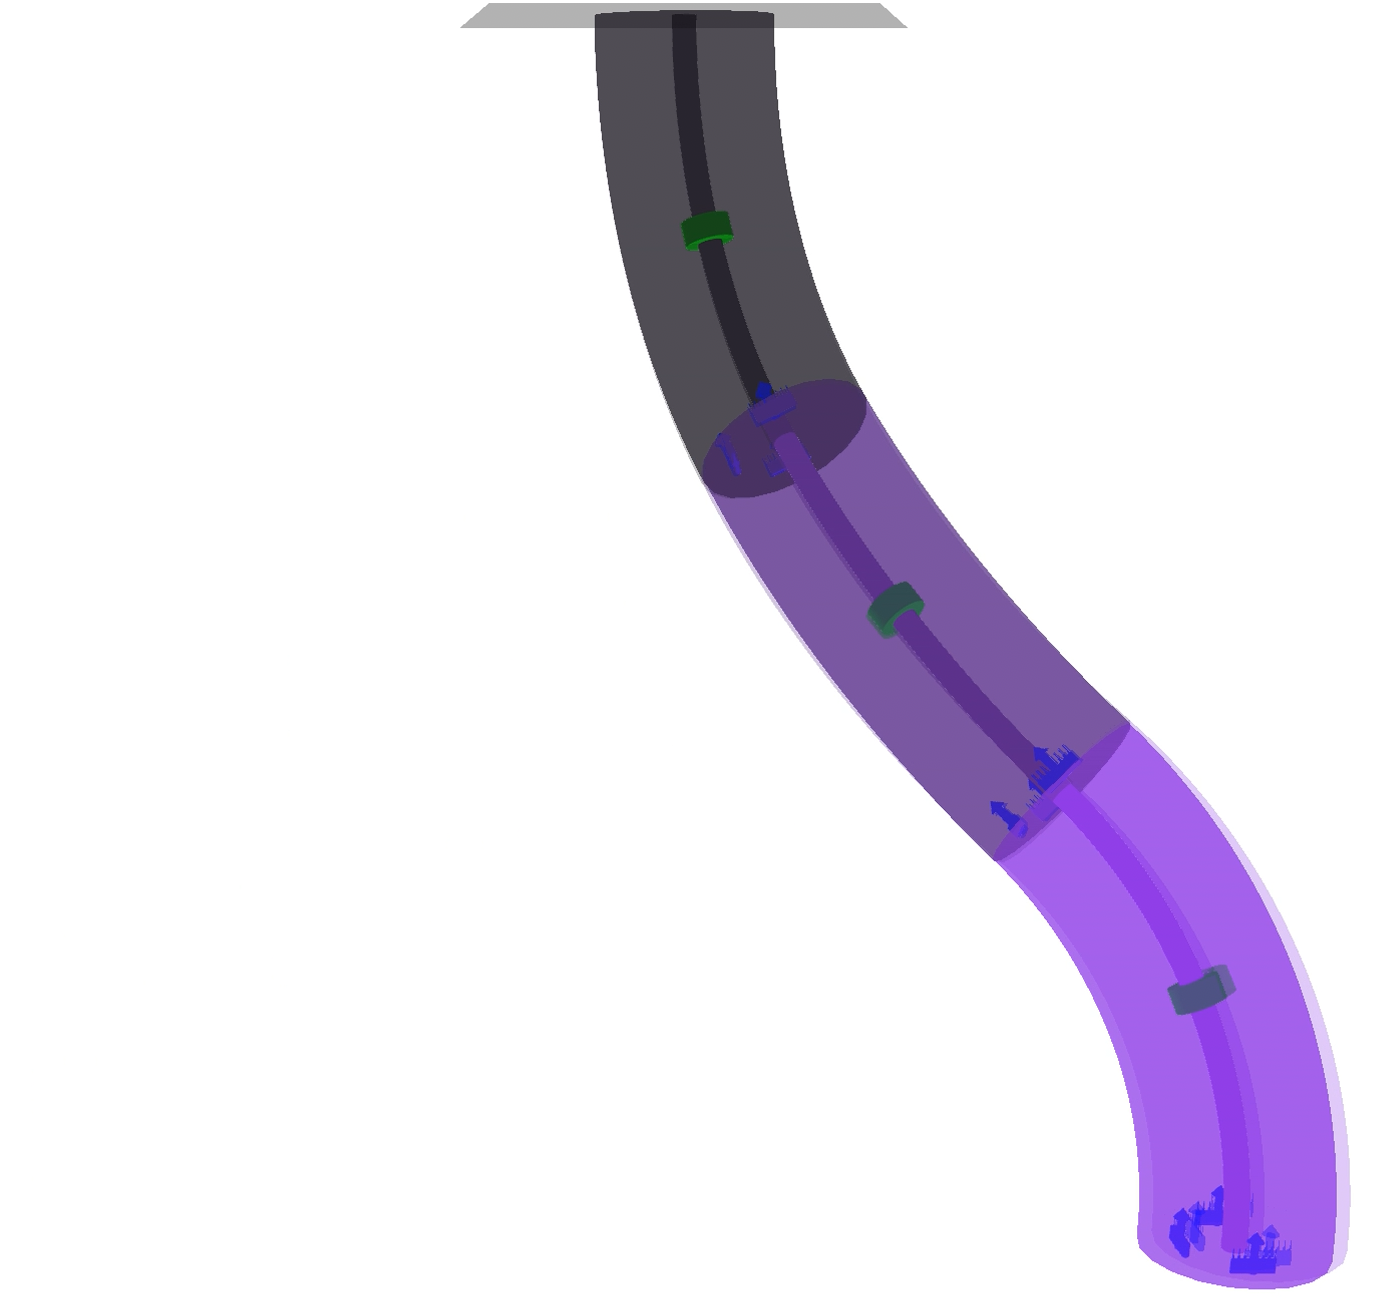
\includegraphics[width=0.161\textwidth]{promasens/figures/simulation_sequences/pcc_simulated_sensor_failure/simulated_sensor_failure_t=6s_cropped.png}}
  \hfill
  \subfigure[$t=\SI{8}{s}$]{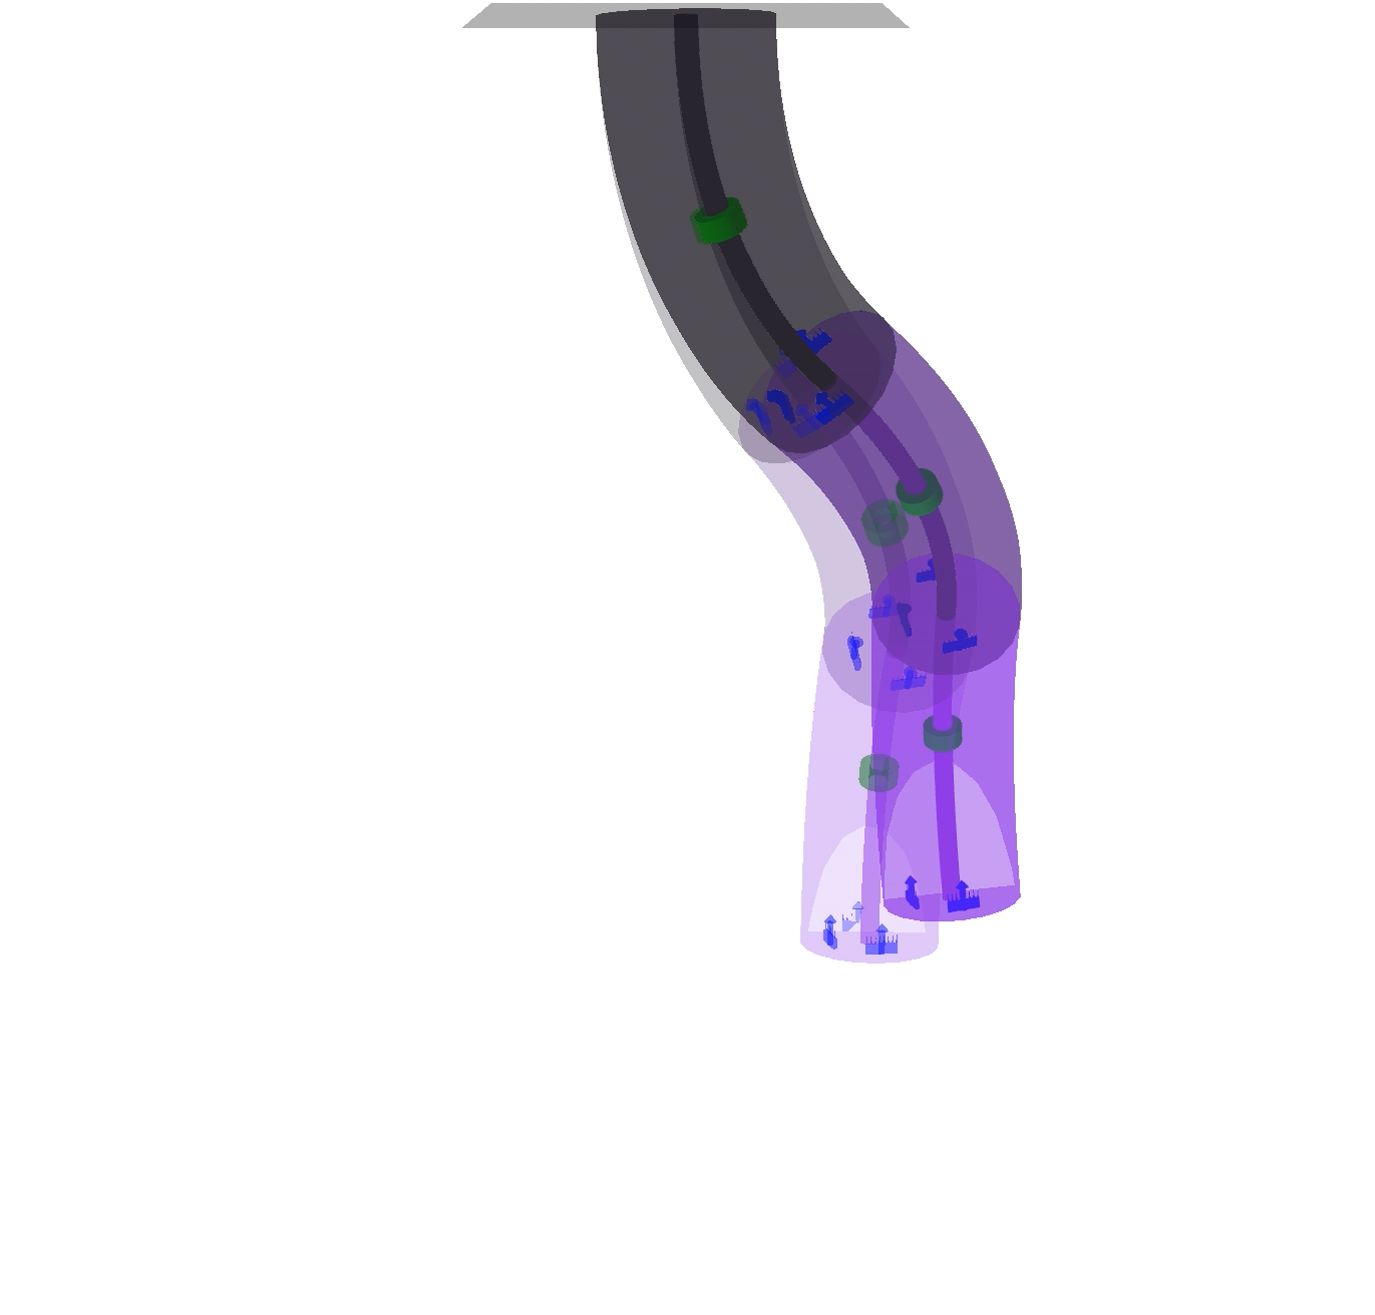
\includegraphics[width=0.161\textwidth]{promasens/figures/simulation_sequences/pcc_simulated_sensor_failure/simulated_sensor_failure_t=8s_cropped.png}}
  \hfill
  \subfigure[$t=\SI{10}{s}$]{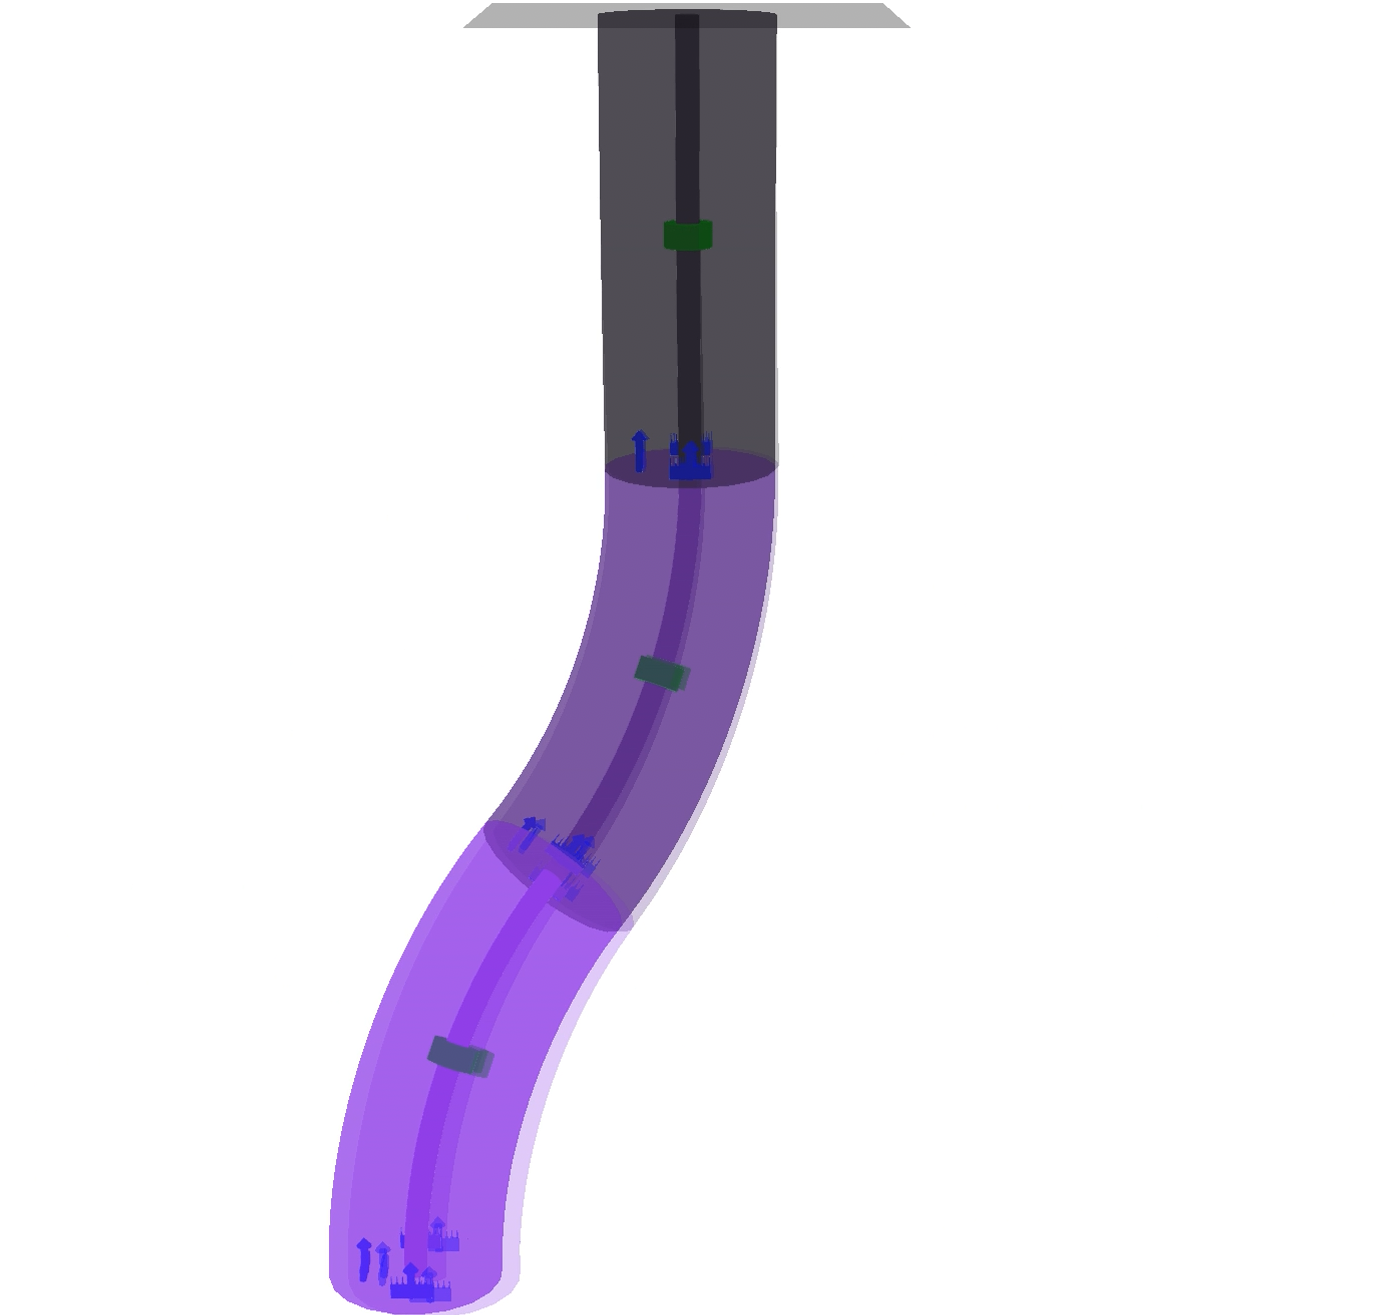
\includegraphics[width=0.161\textwidth]{promasens/figures/simulation_sequences/pcc_simulated_sensor_failure/simulated_sensor_failure_t=10s_cropped.png}}
  % 1375px x 1315px
  \caption{Sequence of stills for simulated sensor failure as shown in Figure~\ref{fig:promasens:simulated_sensor_failure}: the number of sensors per segment, which are rendered in blue, is reduced from four to three at $t=\SI{5}{s}$. We visualize the ground-truth shape of the soft robot with full opacity and the estimated configuration with slight transparency. The magnets are rendered in green and the three segments are visualized in a color sequence from black to violet.}
  \label{fig:promasens:simulation_sequences}
\end{figure*}

\subsection{Optimization}
We optimize the configuration variables $\hat{q}_i = (\hat{\Delta}_{x,i}, \hat{\Delta}_{y,i}, \hat{\delta} L_{i})^\mathrm{T}$ for each segment to minimize the sensor measurement prediction loss as defined in \eqref{eq:promasens:proprioception_loss}.
The optimization strategy solely relies on gradient descent and uses the best solution from the last time step $\hat{q}^*(t-1)$ as an initialization $\hat{q}_0(t)$. For the first time step of the trajectory, we initialize with the ground truth.
We use a step size $\gamma = 3.5 \cdot 10^{-4}$, $3 \cdot 10^{-3}$, and $2 \cdot 10^{-3}$ during gradient descent for a one-segment, two-segment and three-segment robot respectively. For all robots with more than one segment, the step size is reduced by a factor of ten when optimizing the elongation. The momentum $\mu$ is $0.3$ for all trials and we perform $20$ gradient descent iterations for each time step.

\subsection{Evaluation}\label{sub:promasens:pcc_simulations:evaluation}
We evaluate the performance of our method at estimating the configuration of the segment by computing a relative Root Mean-Squared Error (RMSE) metric with respect to the ground-truth configuration $q(t)$ for each configuration variable separately
\begin{equation}\label{eq:promasens:relative_RMSE}
\begin{split}
    e_{q_\star} = \frac{\sqrt{\sum_{t=0}^{n_\mathrm{t}} \left ( \hat{q}_\star(t) - q_\star(t) \right )^2}}{\sqrt{n_\mathrm{t}} \; D_{q_\star}},\\
    % e_{\Delta_y} = \frac{\sqrt{\sum_{t=0}^{n_\mathrm{t}} \left ( \hat{\Delta}_y(t) - \Delta_y(t) \right )^2}}{\sqrt{n_\mathrm{t}} \; L_{\Delta_y}},\\
    % e_{\delta L} = \frac{\sqrt{\sum_{t=0}^{n_\mathrm{t}} \left ( \delta \hat{L}(t) - \delta L(t) \right )^2}}{\sqrt{n_\mathrm{t}} \; L_{\delta L}},
\end{split}
\end{equation}
where $n_\mathrm{t}$ is the number of discrete time-steps and $D_{q_\star}$ is the dynamic range of each configuration variable between the maximum and minimum value in the test set.
All simulations are evaluated on a full lemniscate trajectory, which is very similar to what is plotted based on experimental data in Fig.~\ref{fig:promasens:t3_viz}. The maximum bending angle of this trajectory is \SI{45}{\degree} and the elongation of the segment follows a cosine wave with a minimum and maximum at \SI{1.25}{\percent} and \SI{3.75}{\percent} respectively.

\subsection{Results}\label{sub:promasens:simulation_pcc_results}
We present all simulation results in Tab.~\ref{tab:results_pcc_simulations}.
In the first section, robots with one to three segments, which all exhibit a nominal sensor placement, are considered separately. Neural networks are trained separately for each of these robots, as the input dimension needs to be adjusted to the number of magnets.
% We plot the configuration estimates for the three-segment robot in Fig.~\ref{fig:promasens:simulations_plot}.
The results show that the method works well for robots with 1-3 segments. It can be observed that the estimation error is usually lower for the distal segment(s).

Next, the number of sensors $n_\mathrm{s}$ is varied for a three-segment robot. We always apply a symmetrical placement of the sensors in the tip plane of each segment. In the first trial, two sensors are mounted in the tip plane of each segment opposite to each other (6 sensors in total). While the bending along $\Delta_{x,i}$ and the elongation of the segments $\delta L_i$ can still be estimated, the setup does not contain sufficient information to accurately determine the bending into $\Delta_{y,i}$.
While the nominal case of nine sensors in total already achieves relative RMSEs in the range of \SI{1.6}{\percent} to \SI{6}{\percent}, the proprioception performance can be slightly improved by adding more sensors.
% Recall that no re-training of the neural network is required when adding or removing sensors.
We emphasize that the neural networks are not retrained when adding or removing sensors.
In Figures~\ref{fig:promasens:simulated_sensor_failure} and \ref{fig:promasens:simulation_sequences}, we plot the proprioceptive performance of a three-segment robot with four sensors per segment. Then, we simulated a failure of the 4th, 8th, and 12th sensor at \SI{5}{s} by removing these sensor measurements from \eqref{eq:promasens:gradient_descent} (i.e. the gradient descent). Our method is able to adapt without re-training and leverage the nominal redundancy of sensor measurements, as three sensors per segment are sufficient for shape estimation.

Then, two adjusted sensor placements are investigated, while keeping the neural network weights constant. First, the sensors are tilted from the nominal case of pointing along the local z-axis by $\psi_\mathrm{s} = \SI{10}{\degree}$ towards the inside. In a separate simulation, the sensors are moved radially from nominally \SI{13}{mm} to \SI{16}{mm}. As the results show, the configuration of all three segments can still be estimated accurately with a mean error of \SI{3.3}{\percent}.

Finally, an earth's magnetic field of magnitude \SI{0.065}{mT} is added. A separate neural network is trained on a training set with randomly sampled magnetic field vector directions $n_\mathrm{e}$. As the last section of Tab.~\ref{tab:results_pcc_simulations} demonstrates, the methodology is able to adapt to any earth's magnetic field direction by leveraging the $\lambda_j$ input parameter.

% \subsection{Synthetic results}\label{sub:promasens:synthetic_results}
% We initially verify and quantitatively compare our method with an end-to-end trained neural network using a synthetic sensor measurement model: \textcolor{red}{Insert citation why we are using this synthetic sensor measurement model and also describe the \gls{NN} and how it differs from \gls{NN} from our method}
% \begin{equation}
%     u_j = \sum_{k=1}^{n_\mathrm{m}} \frac{1000}{d_{jk}^2} \cdot \cos( \theta_{jk}) \cdot \cos( \beta_{jk}) + n_u
% \end{equation}

% Alternatively, we implement a more realistic, analytical 2D model for the magnetic flux intensity of one magnet $k$ measured by sensor $j$. As our segment is axially symmetric, we can a 2D magnetic flux model in the plane of the angle $\theta_{jk}$. Referring to \eqref{eq:promasens:d_jk} and \eqref{eq:promasens:theta_jk}, we define the radial and axial distance between the magnet and the sensor as:
% \begin{equation}
%     d_{a,jk} = \cos(\theta_{jk}) \cdot d_{jk} \qquad d_{r,jk} = \sin(\theta_{jk}) \cdot d_{jk}
% \end{equation}
% For a magnet with thickness $h_m$ and of diameter $D_m$ in a medium with a relative magnetic permeability $\mu_o$ (for air $1.00000037$) and $M_a$ the surface magnetization magnitude of the magnet, we can define the magnetic field vector components in the cylindrical coordinate system of the magnet $jk$ as~\cite{furlani2001permanent, ozel2015precise}:
% \begin{equation}\scriptsize
% \begin{split}
%     B^a(d_a, d_r) = \frac{\mu_0 M_x}{2 \pi} \Bigg ( & \quad \arctan \frac{2 h_m \cdot (d_a + D_m)}{(d_a + D_m)^2 + d_r^2 - h_m^2} \\ 
%     & - \arctan \frac{2 h_m \cdot (d_a - D_m)}{(d_a - D_m)^2 + d_r^2 - h_m^2} \Bigg ),\\
%     B^r(d_a, d_r) = \frac{\mu_0 M_x}{2 \pi} \Bigg ( & \quad \ln \frac{(d_a + D_m)^2 + (d_r - h_m)^2 }{(d_a + D_m)^2 + (d_r + h_m)^2} \\ 
%     & - \ln \frac{(d_a - D_m)^2 + (d_r - h_m)^2 }{(d_a - D_m)^2 + (d_r + h_m)^2}  \Bigg ).
% \end{split}
% \end{equation}
% We rotate the translation between the magnet and the sensor into the magnet frame $\{S_{\mathrm{m}_k}\}$ and project it into the local x-y plane:
% \begin{equation}
%     t_{\mathrm{m}_k,xy}^{jk} = 
%     \mathrm{diag}(\begin{bmatrix} 1 & 1 & 0 \end{bmatrix}) 
%     \cdot (R_{i-1}^{\mathrm{m}_k})^{\mathrm{T}} \cdot t_{i-1}^{jk},
% \end{equation}
% which allows us to define the magnetic field vector in the frame $\{ S_{\mathrm{m}_k} \}$:
% \begin{equation}
%     B_{\mathrm{m}_k}^{jk} = 
%     \begin{bmatrix}
%         \frac{x^{t_{jk}}_{\mathrm{m}_k,xy}}{\lVert  t_{\mathrm{m}_k,xy}^{jk} \rVert} \cdot B^{r,jk} & \frac{y^{t_{jk}}_{\mathrm{m}_k,xy}}{\lVert  t_{\mathrm{m}_k,xy}^{jk} \rVert} \cdot B^{r,jk} & B^{a,jk}
%     \end{bmatrix}^{\mathrm{T}}.
% \end{equation}
% Next, we compute the expected sensor measurement $u_j$ using the scalar projection of the magnetic field vector $B_{i-1}^{jk}$ along the sensor measurement unit vector $\{ \hat{o}_{\mathrm{s}_j} \}_{i-1}$ with the dot product as:
% \begin{equation}
%     u_j = \sum_{k=1}^{n_\mathrm{m}} \left ( R_{i-1}^{\mathrm{m}_k} \cdot B_{\mathrm{m}_k}^{jk} \right ) \cdot \{ \hat{o}_{\mathrm{s}_j} \}_{i-1}
% \end{equation}

% We apply both input and process Gaussian noise to pose a realistic challenge for both proprioception methods.
% \textcolor{red}{Please insert the correct noise values here:}
% We add the process noise $n_u \sim \mathcal{N}\left(\SI{0.2}{V}, \SI{0.5}{V} \right)$ to the target sensor measurement $u$ and the inputs noise $n_d \sim \mathcal{N}\left(\SI{0.2}{m}, \SI{0.5}{m} \right)$, $n_\theta \sim \mathcal{N}\left(\SI{0.2}{\degree}, \SI{0.5}{\degree} \right)$ and $n_\beta \sim \mathcal{N}\left(\SI{0.2}{\degree}, \SI{0.5}{\degree} \right)$ before $\Bar{\xi}$ is passed to the neural network:
% \begin{equation}
%     \Bar{\xi}_{jk} = \xi_{jk} + 
%     \begin{bmatrix}
%     n_d & n_\theta & n_\beta
%     \end{bmatrix}^\mathrm{T}
% \end{equation}

\section{Affine Curvature Simulations}\label{sec:promasens:ac_simulations}
To demonstrate the efficacy of the proposed method for higher-order kinematic models than \gls{PCC}, we also conduct simulations of an \gls{AC} soft robot.
The \gls{AC} kinematic parametrization~\citep{della2020soft} has been shown capable of representing the shape of soft tentacles~\citep{stella2022experimental, stella2023piecewise} and provides a continuous function $\kappa = \kappa_0 + \kappa_1 \: v$ to describe the curvature of the soft robot, where $\kappa_0$, $\kappa_1$ are two configuration variables and $v \in [0, 1]$ is the backbone coordinate. We allow for movement in 3D space by also specifying an azimuth bending angle $\phi$ and the elongation $\delta L$.
Please refer to Section~\ref{sub:promasens:kinematic_model_ac} for more implementation details about the \gls{AC} model.


\subsection{Simulation Setup}\label{sub:promasens:ac_simulations:simulation_setup}
We use the same simulation setup as described in Section~\ref{sub:promasens:pcc_simulations:simulation_setup}. 
Therefore, we report in the following only the implemented modifications to simulate an \gls{AC} soft robot in Magpylib~\citep{magpylib2020}.
Namely, we consider one \gls{AC} segment of length $L_{0,i} = \SI{200}{mm}$ with in total $n_\mathrm{s} = 9$ magnetic sensors. 
The sensors are placed on three separate cylindrical planes at distances $d_{\mathrm{s}_\mathrm{a}}$ of \SI{0}{mm}, \SI{100}{mm}, and \SI{200}{mm} from the base of the robot. In each plane, the three sensors are spaced at an angle of \SI{120}{\degree} and at a radial distance $d_{\mathrm{s}_\mathrm{r}} = \SI{13}{mm}$ from the backbone, as it can be seen in Fig.~\ref{fig:promasens:ac_simulations:inference_sequences}.
Two ring magnets are positioned at a distance of \SI{50}{mm} and \SI{150}{mm} from the robot's base, respectively.

\begin{figure}[hbt]
  \centering
  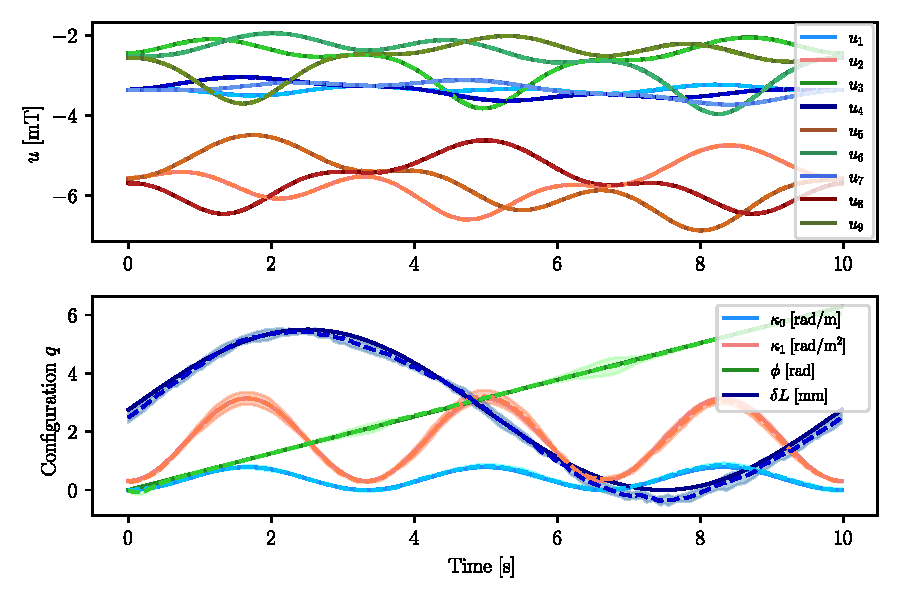
\includegraphics[width=0.8\columnwidth]{promasens/figures/simulation_results/ac/affine_curvature_inference_v2_cropped.pdf}
  \caption{Sensor measurement predictions (top) and configuration estimates (bottom) for an \gls{AC} segment with nine magnetic sensors. We plot the ground-truth values $u$ and $q$ in solid, the estimate $\hat{u}$ and $\hat{q}$ as a mean over three random seeds with dashed lines and the standard deviation as an error band. The random seed determines the initialization of the neural network weights at the start of the training.}
  \label{fig:promasens:ac_simulations:inference_plot}
\end{figure}

\begin{figure*}[hbt]
  \centering
  \subfigure[$t=\SI{0}{s}$]{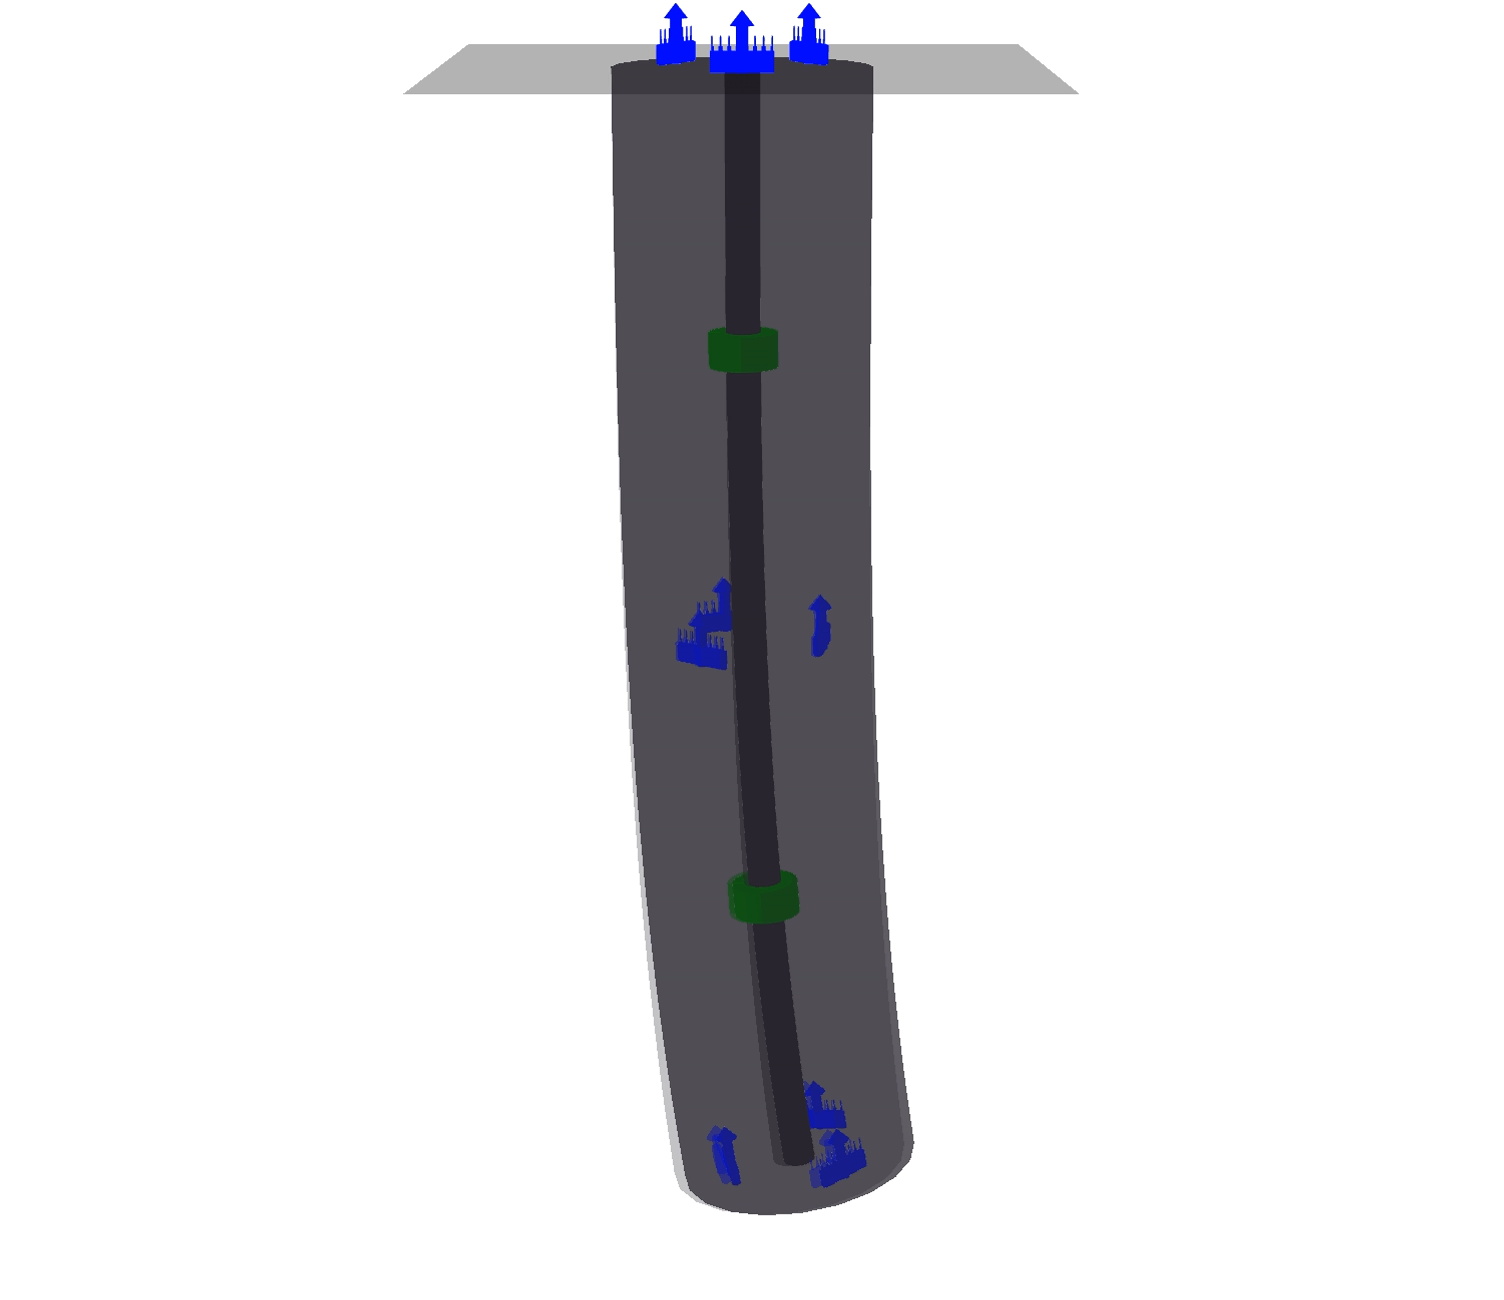
\includegraphics[width=0.161\textwidth]{promasens/figures/simulation_sequences/ac_flower_trajectory/affine_curvature_flower_t=0s_cropped.png}}
  \hfill
  \subfigure[$t=\SI{2}{s}$]{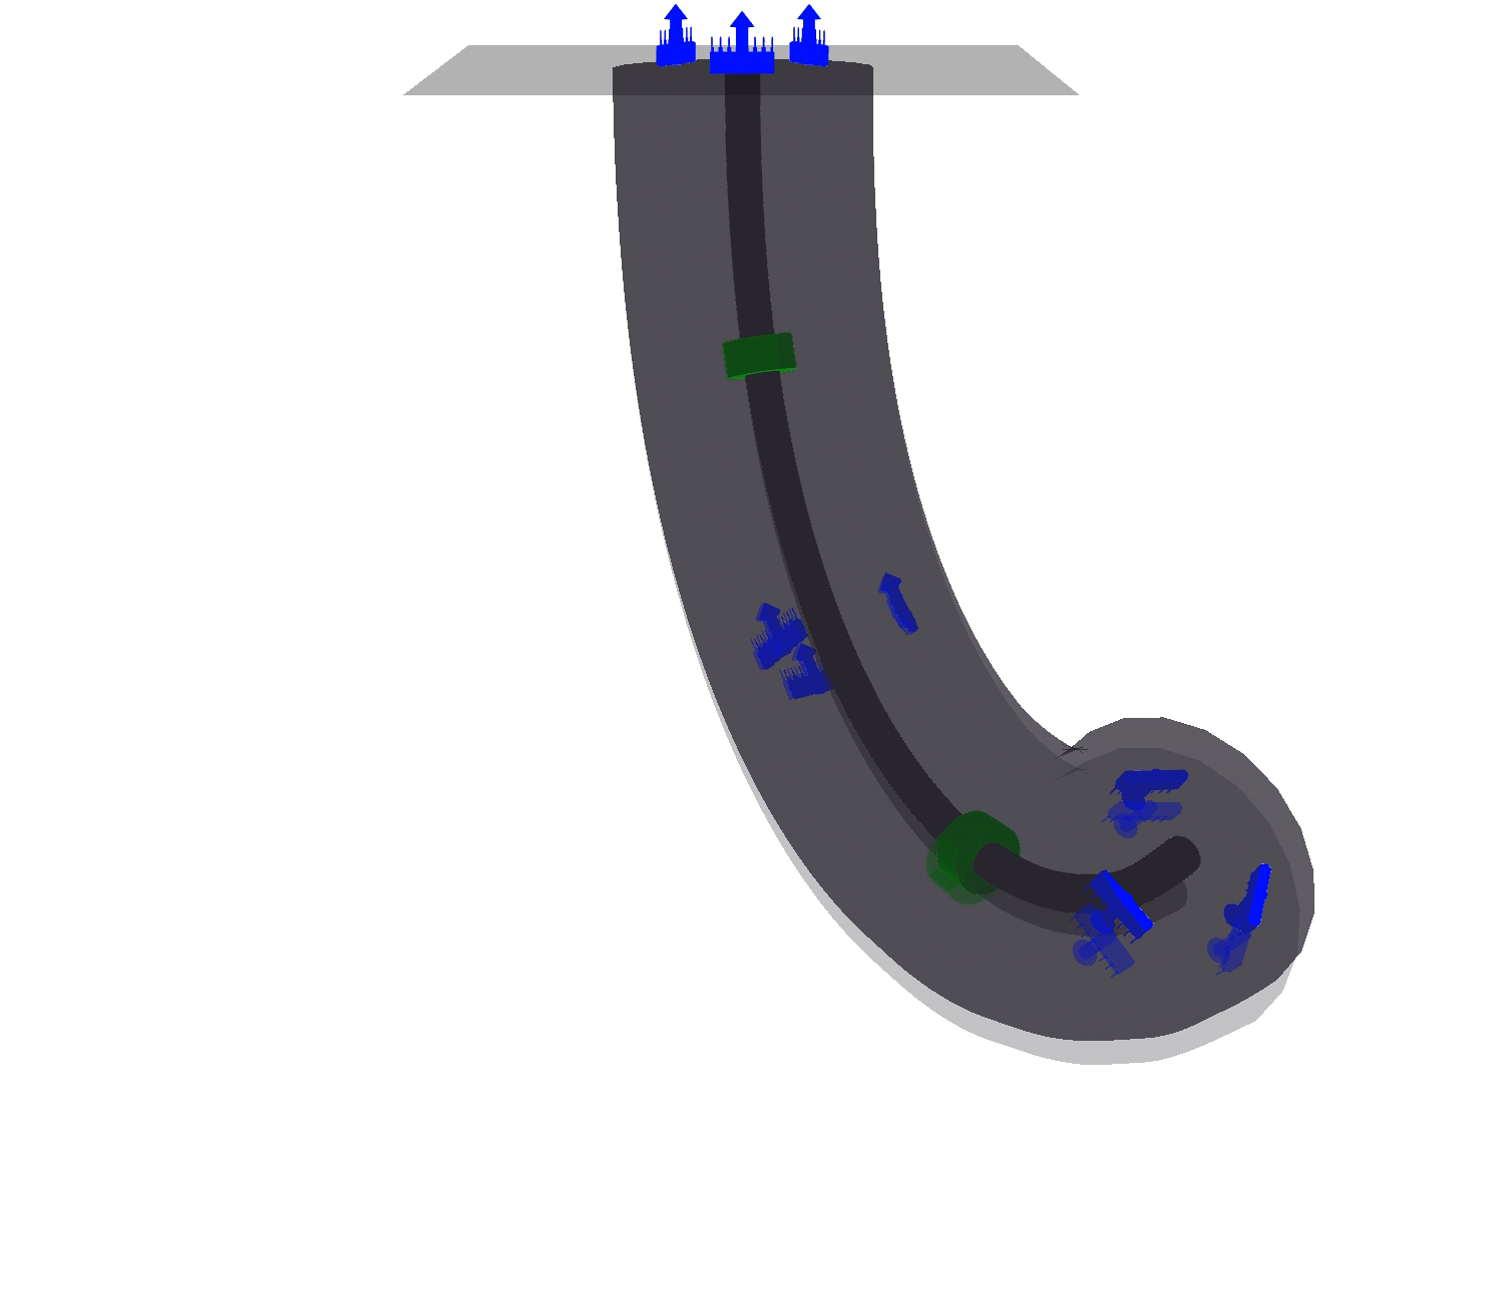
\includegraphics[width=0.161\textwidth]{promasens/figures/simulation_sequences/ac_flower_trajectory/affine_curvature_flower_t=2s_cropped.png}}
  \hfill
  \subfigure[$t=\SI{4}{s}$]{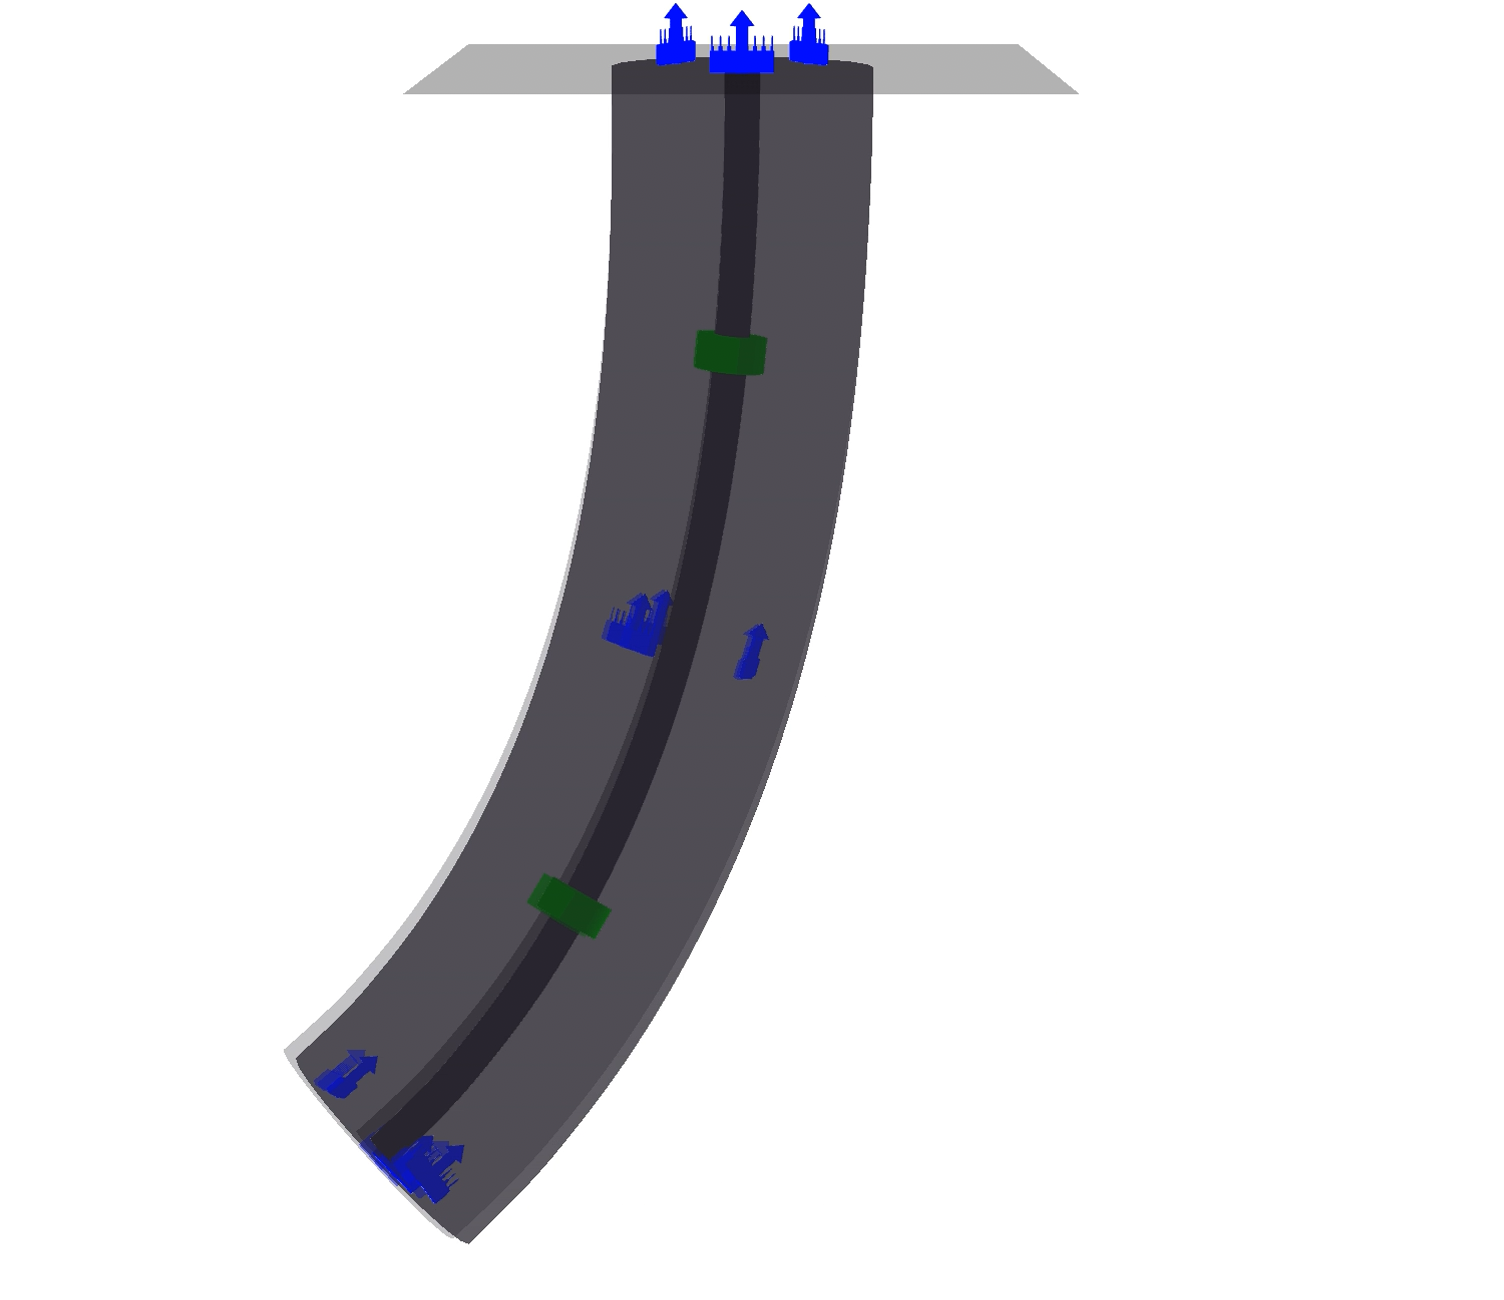
\includegraphics[width=0.161\textwidth]{promasens/figures/simulation_sequences/ac_flower_trajectory/affine_curvature_flower_t=4s_cropped.png}}
  \hfill
  \subfigure[$t=\SI{6}{s}$]{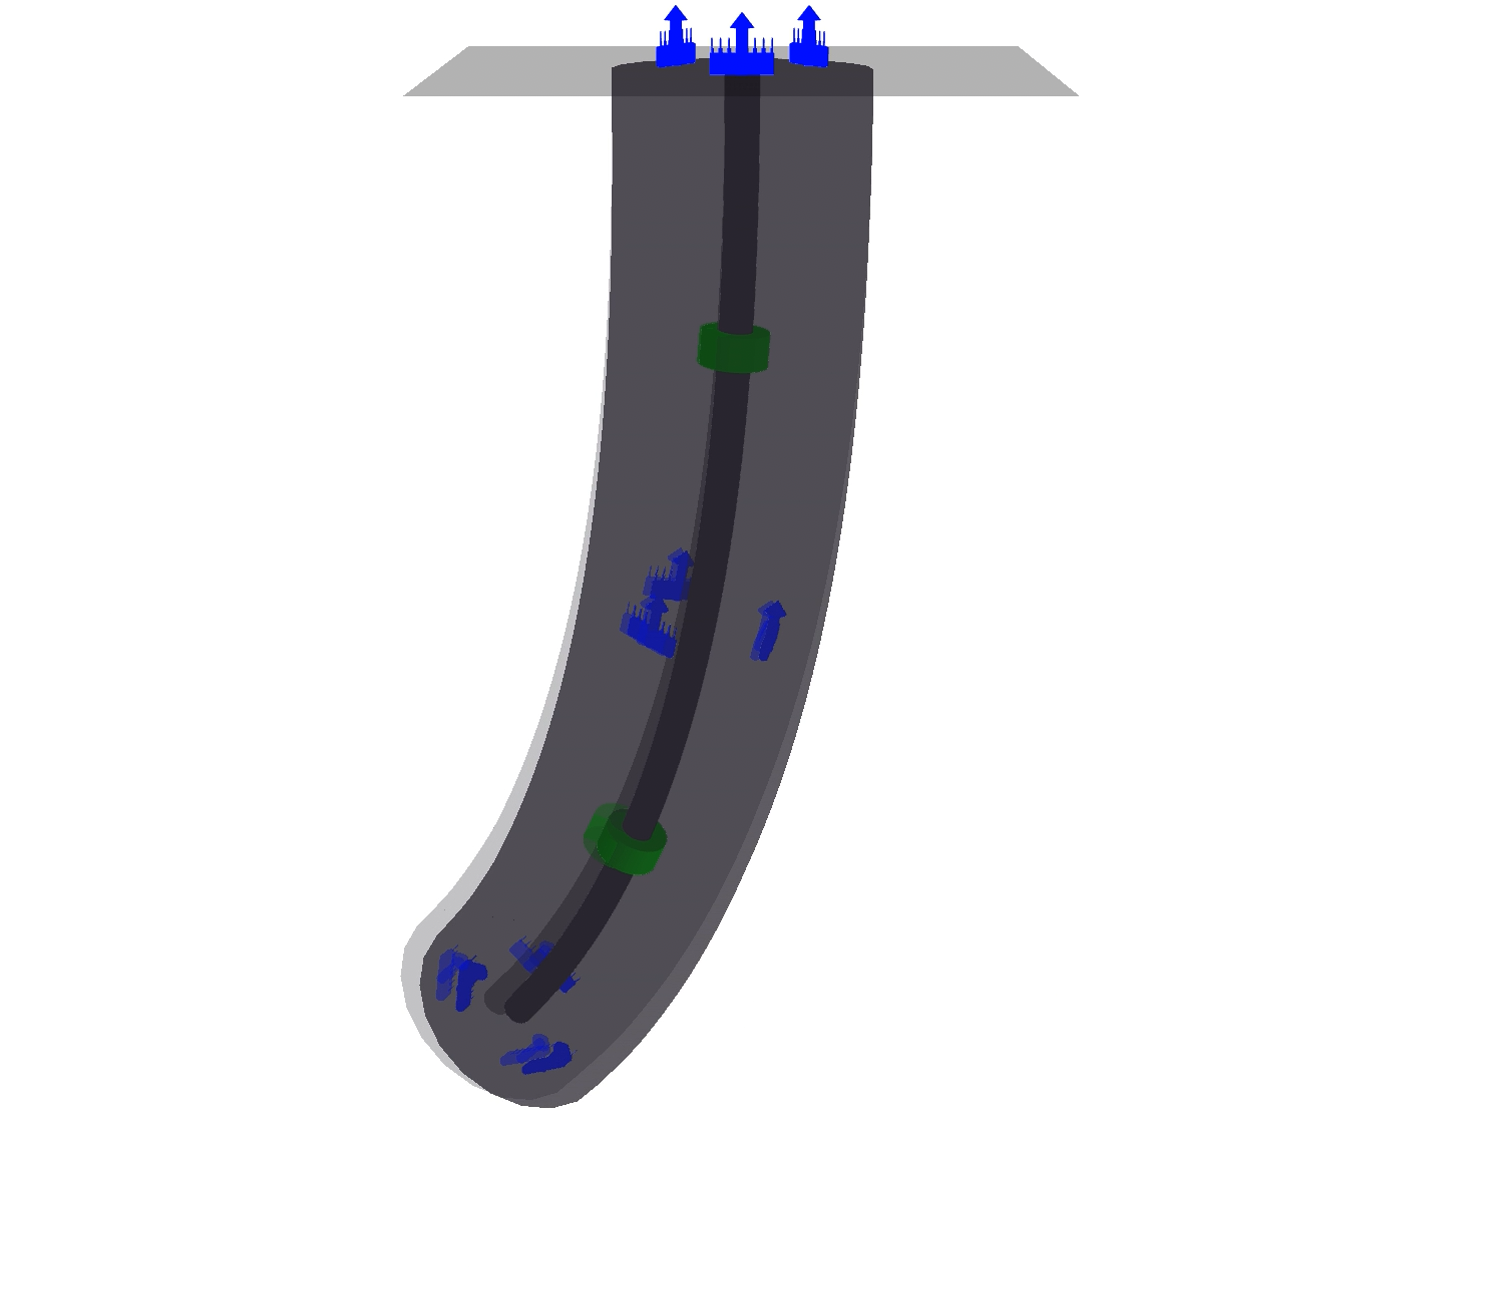
\includegraphics[width=0.161\textwidth]{promasens/figures/simulation_sequences/ac_flower_trajectory/affine_curvature_flower_t=6s_cropped.png}}
  \hfill
  \subfigure[$t=\SI{8}{s}$]{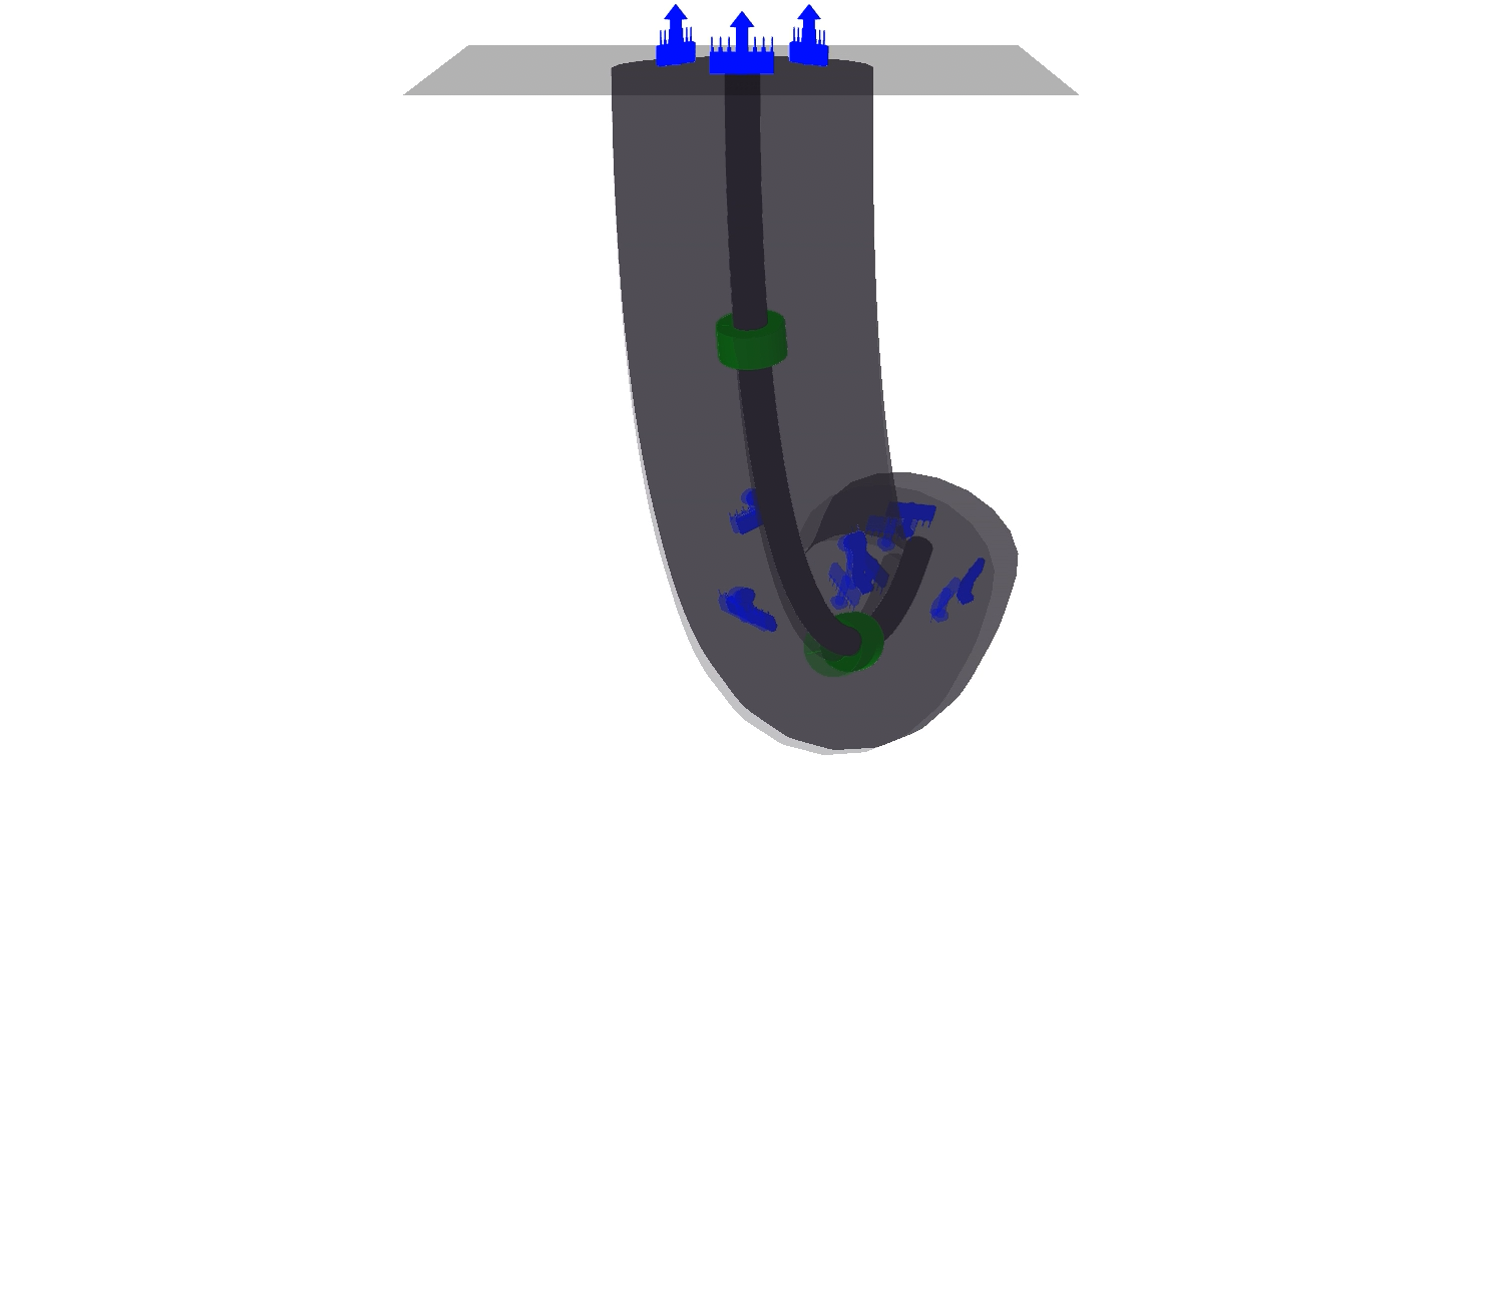
\includegraphics[width=0.161\textwidth]{promasens/figures/simulation_sequences/ac_flower_trajectory/affine_curvature_flower_t=8s_cropped.png}}
  \hfill
  \subfigure[$t=\SI{10}{s}$]{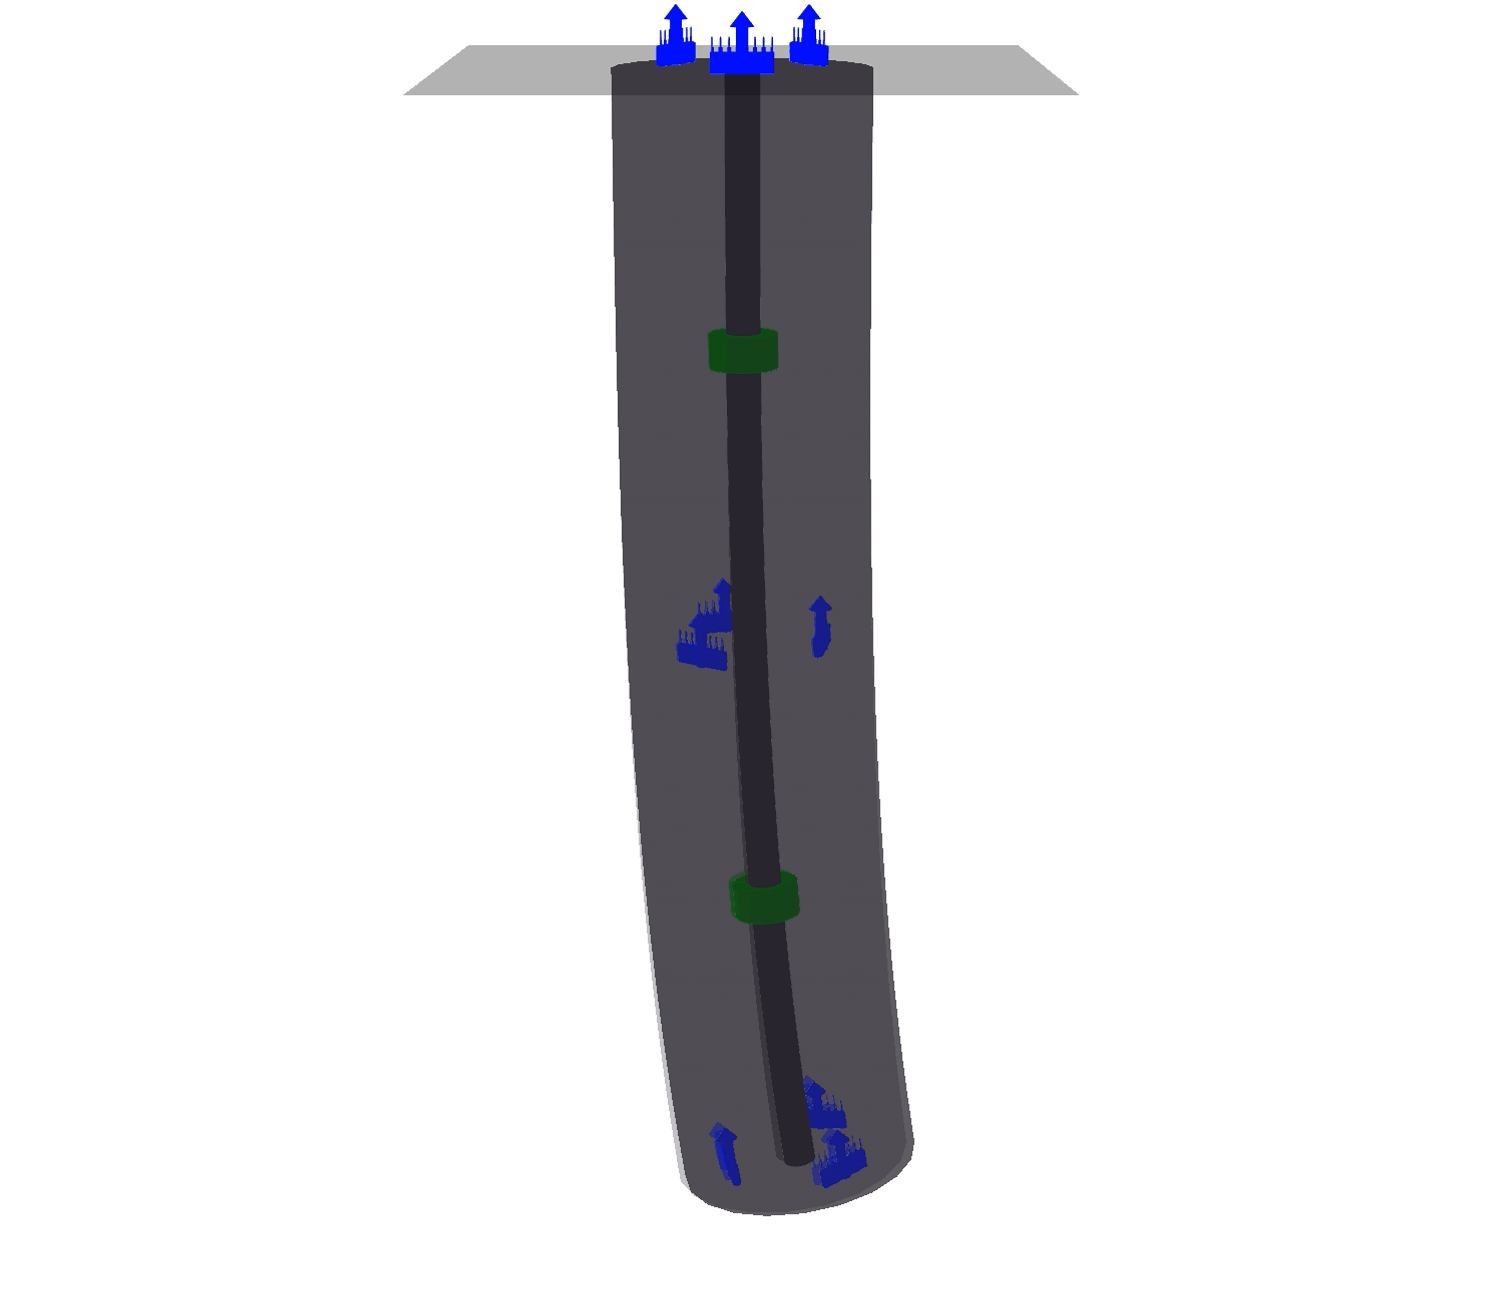
\includegraphics[width=0.161\textwidth]{promasens/figures/simulation_sequences/ac_flower_trajectory/affine_curvature_flower_t=10s_cropped.png}}
  % 1504 x 1400px
  \caption{Sequence of stills for a simulated \gls{AC} robot. We visualize the ground-truth shape of the soft robot with full opacity and the estimated configuration with slight transparency. The two magnets are rendered in green and the nine sensors in blue.}
  \label{fig:promasens:ac_simulations:inference_sequences}
\end{figure*}

\subsection{Prediction Network and Optimization}\label{sub:promasens:ac_simulations:network_optimization}
We simulate \SI{120000}{} random configurations of the \gls{AC} robot to generate the training set. For this purpose, we sample the configuration variables from uniform distributions: the \gls{AC} parameters $\kappa_0 \in \mathcal{U}(0, \SI{0.942}{rad \per m})$, $\kappa_1 \in \mathcal{U}(0, \SI{3.770}{rad \per m^2})$, the azimuth angle $\phi \in \mathcal{U}(0, 2 \pi \: \si{rad})$, and the elongation $\delta L \in \mathcal{U}(0, \SI{6.6}{mm})$.
Before training, we randomly split off \SI{30}{\percent} of the training set for validation purposes.
We train a specialized neural network $f_{\pi_j(\xi_j)}$ for each sensor and use the same neural network architecture as in Section~\ref{sub:promasens:pcc_simulations:neural_network} with the exception of the addition of a final layer $y(x) = \mathrm{sign}(x) \: e^{|x|}$. 
The training runs for a total of $250$ epochs and uses the SWA~\citep{izmailov2018averaging} strategy with a learning rate of $0.01$. 
All other training hyperparameters are the same as in Section~\ref{sub:promasens:pcc_simulations:neural_network}.

The four configuration variables are optimized to minimize the loss between the predictions and simulated measurements of the nine sensors as defined in \ref{eq:promasens:proprioception_loss}.
For this optimization procedure, we employ gradient descent running at \SI{40}{Hz} with step sizes of $\gamma_{\kappa_0} = 1$, $\gamma_{\kappa_1} = 5$, $\gamma_{\phi} = 1$, and $\gamma_{\delta L} = 2 \cdot 10^{-4}$. The momentum is set to $\mu = 0.3$ and $20$ iterations are performed at each time step.

\subsection{Evaluation}\label{sub:promasens:ac_simulations:evaluation}
We evaluate the trained model on a flower trajectory of duration \SI{10}{s} and sample rate \SI{40}{Hz}. The evaluation trajectory has the following characteristics: $\kappa_0$ is actuated by a sinusoidal wave of frequency \SI{0.3}{Hz} in the range $[0, \frac{\pi}{4} \: \si{rad \per m}]$. Similarly, $\kappa_1$ is also varied through a sinusoidal function of the same frequency and has a dynamic range of $[0.1 \pi, \pi] \: \si{rad \per m^2}$.
The azimuth angle $\phi$ is linearly scaled from \SI{0}{rad} to $2 \pi \: \si{rad}$ over the duration of the trajectory.
Finally, $\delta L$ follows a sinusoidal sequence of frequency \SI{0.1}{Hz} in the range of $[0, 5.5] \: \si{mm}$.
We use the same evaluation metrics as first introduced in Section~\ref{sub:promasens:pcc_simulations:evaluation}.
We report the error as mean ± stdev and compute the statistics over three
different random seeds. The random seed determines the initialization of the neural network weights at the start of the training.

\subsection{Results}\label{sub:promasens:ac_simulations:results}
The trained neural networks achieve an RMSE error for predicting the magnetic sensor measurements of $0.025 \pm 0.002 \: \si{mT}$ on the test set.
When we run inference (see Fig.~\ref{fig:promasens:ac_simulations:inference_plot}) on the flower trajectory, the configuration variables can be estimated with an absolute RMSE of $e_{\kappa_0} = 0.042 \pm 0.005 \: \si{rad \per m}$, $e_{\kappa_1} = 0.11 \pm 0.04 \: \si{rad \per m^2}$, $e_{\phi} = 0.08 \pm 0.02 \: \si{rad}$, and $e_{\delta L} = 0.001 \pm 0.001 \: \si{mm}$. 
We state the relative RMSE errors for the configuration estimates as $e_{\kappa_0} = 5.4 \pm 0.7 \: \si{\percent}$, $e_{\kappa_1} = 4.0 \pm 1.4 \: \si{\percent}$, $e_{\phi} = 1.3 \pm 0.4 \: \si{\percent}$, and $e_{\delta L} = 3.8 \pm 1.6 \: \si{\percent}$.
In Fig.~\ref{fig:promasens:ac_simulations:inference_sequences}, we render at six different points along the trajectory the robot's shape according to the ground truth and estimated configurations, respectively.
The sequence qualitatively shows that our proposed method is able to estimate the affine curvature robot's shape very accurately.

\section{Experiments}\label{sec:promasens:experiments}
\begin{figure*}[hbt]
    \centering
    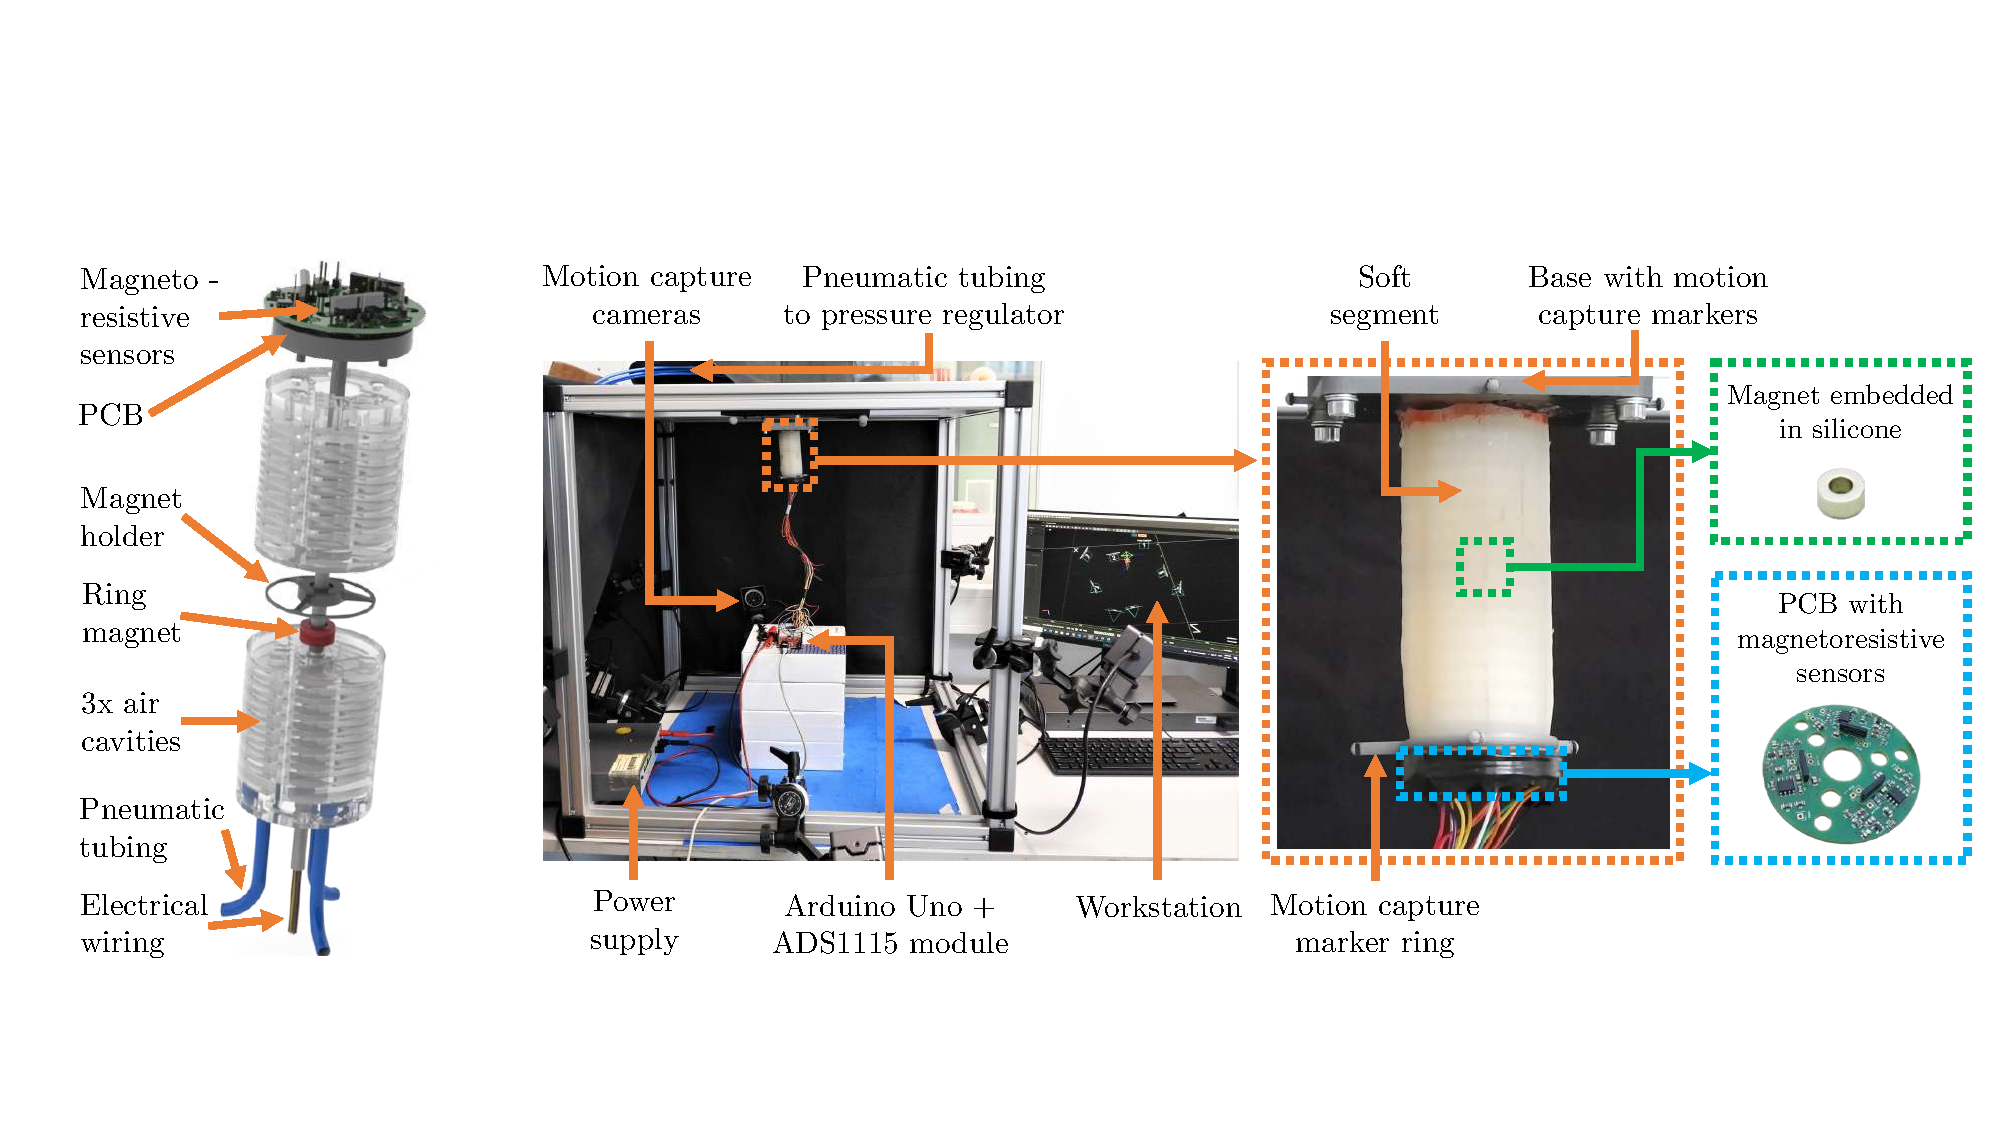
\includegraphics[width=1.0\textwidth]{promasens/figures/experimental_setup/experimental_setup_v5_compressed.pdf}
    \caption{
    \textbf{Left:} Exploded rendering visualizing the robot design with the three magnetoresistive sensors integrated into a PCB at the tip of the segment. The electrical wires from the PCB are passed through the backbone to the base. A ring magnet attached to a 3D-printed holder is integrated into the backbone at a half-segment-length distance from the proximal end. The air chambers of the segment are connected to a pressure regulator via tubing glued at the base of the segment. \textbf{Right:} Experimental setup with the soft robot segment attached in tip-down configuration to the motion capture cage.
    }\label{fig:promasens:experimental_setup}
\end{figure*}
% \begin{figure*}[hbt]
%     \centering
%     \subfigure[Design]{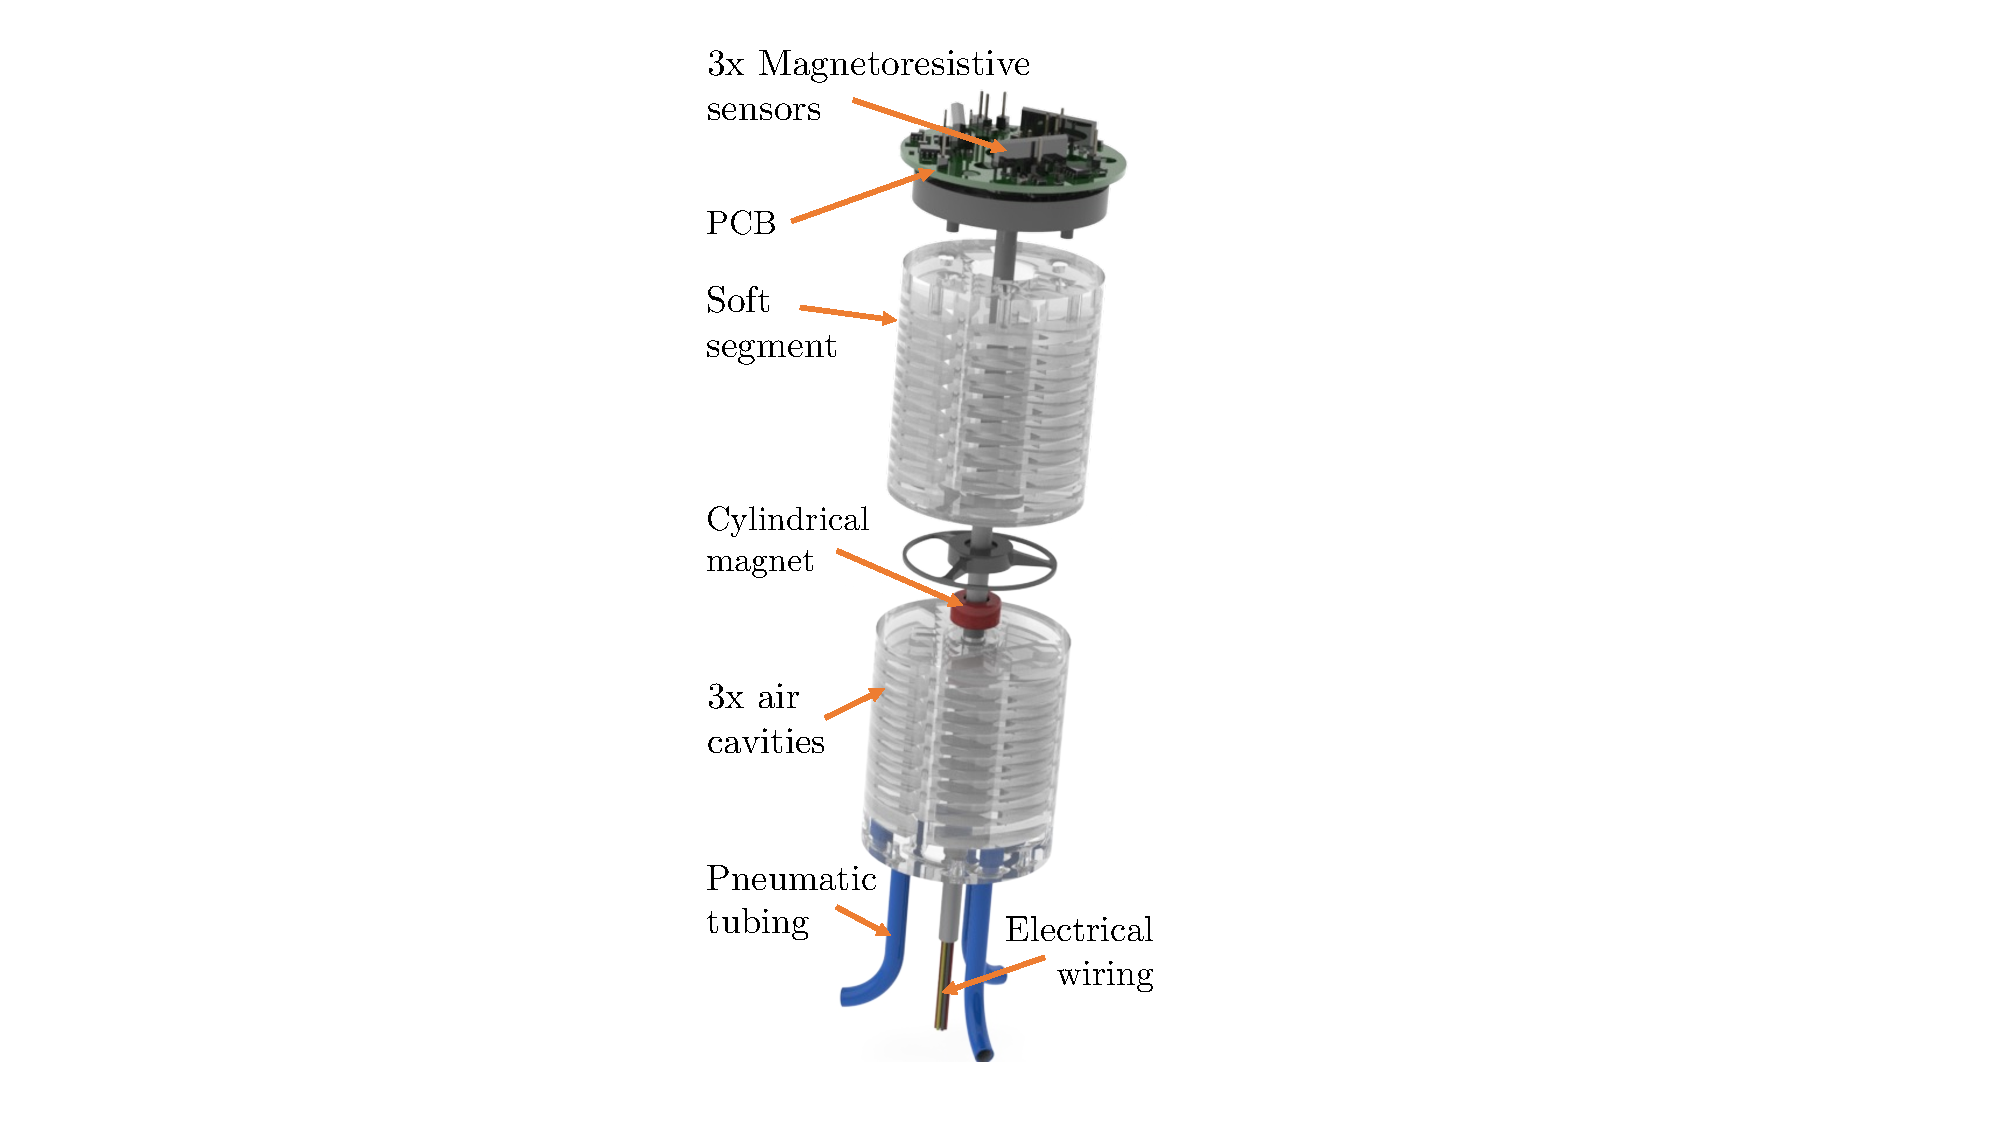
\includegraphics[width=0.135\textwidth]{promasens/figures/segment_design/segment_exploded_rendering_labeled_v1_cropped.pdf}\label{fig:promasens:exploded_rendering}}
    % \hspace{1pt}
%     \hfill
%     \subfigure[Experimental setup]{\includegraphics[width=0.65\textwidth]{promasens/figures/experimental_setup/experimental_setup_v4_compressed.pdf}\label{fig:promasens:experimental_setup}}
%     % \hspace{1pt}
%     \hfill
%     \subfigure[Actuated soft robot]{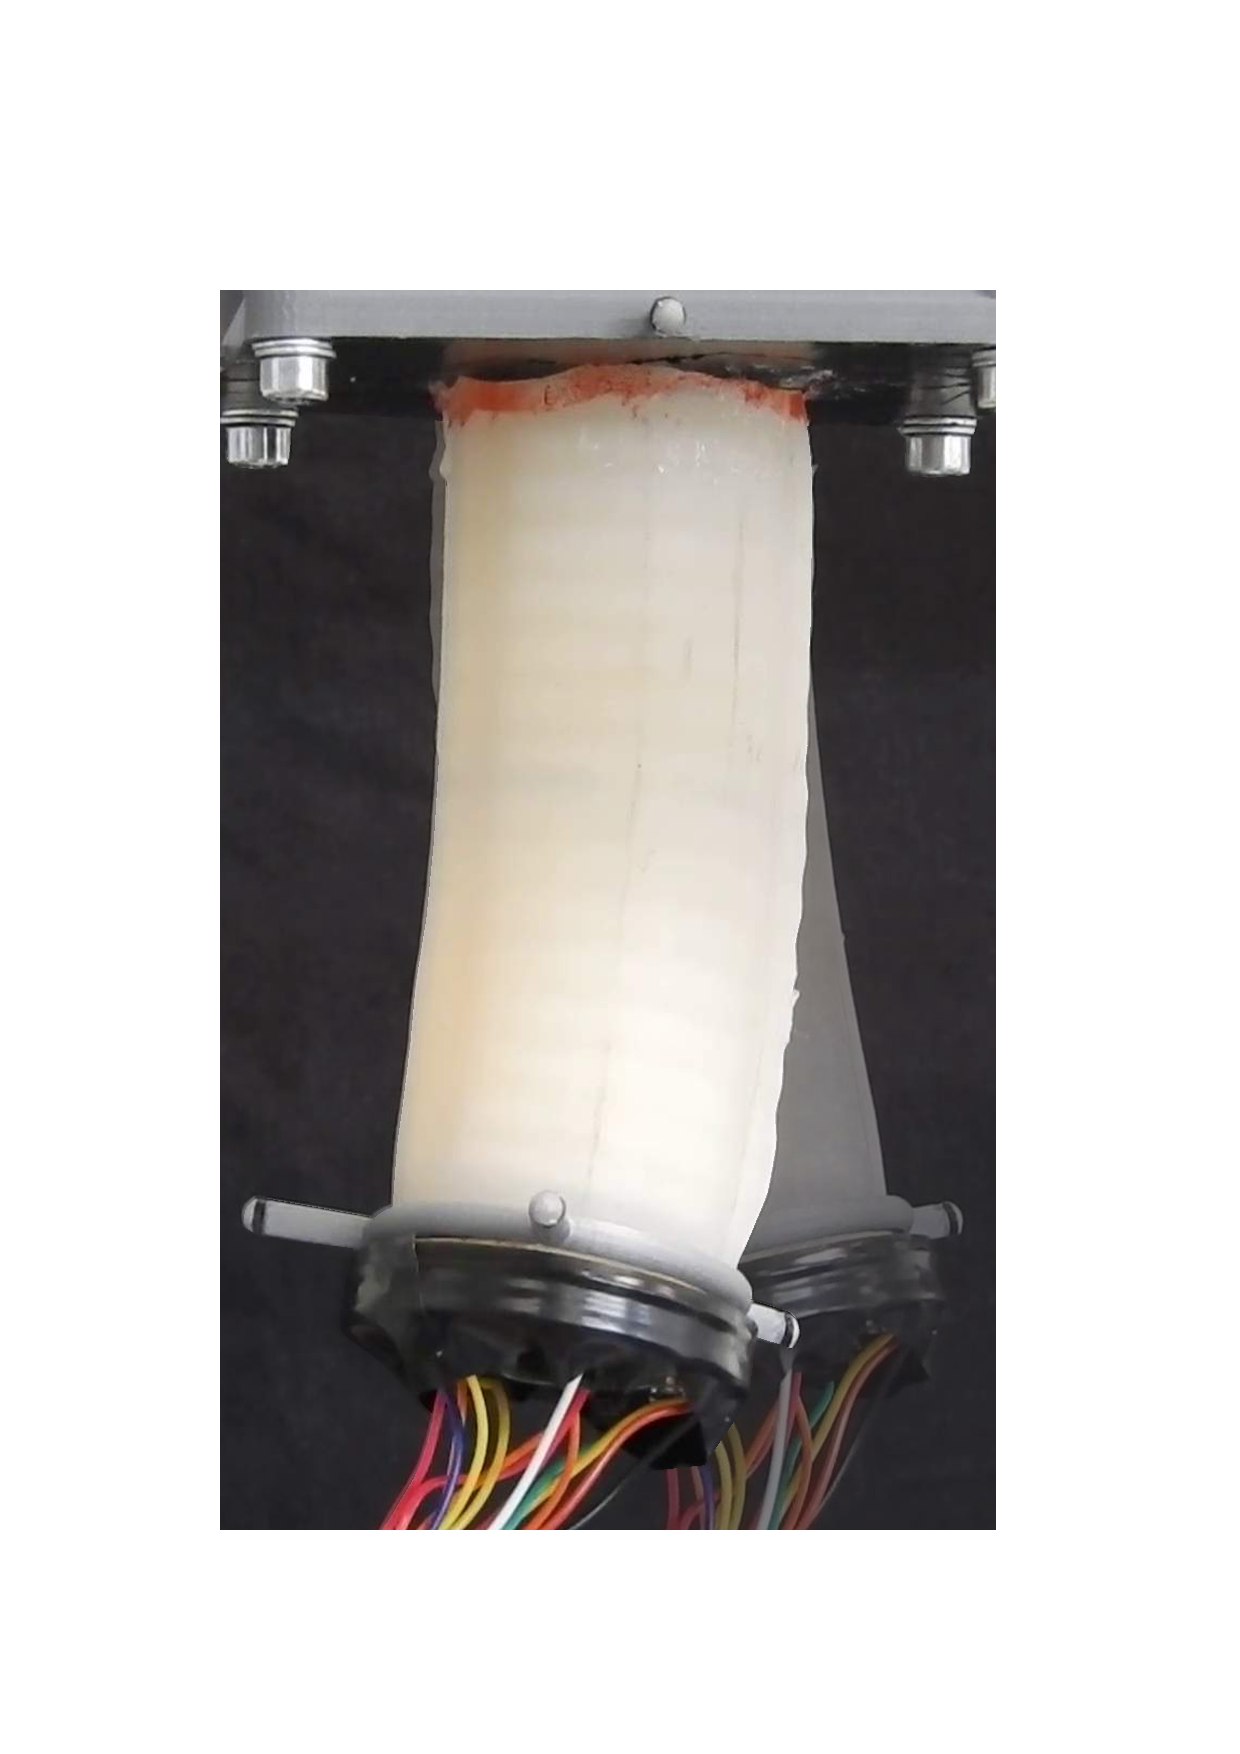
\includegraphics[width=0.16\textwidth]{promasens/figures/robot_bending/Overlapping_images_left_solid_right_transparent_compressed.pdf}\label{fig:promasens:actuated_soft_robot}}
%     \caption{\textbf{Panel (a):} Exploded rendering visualizing the robot design with the three magnetoresistive sensors integrated into a PCB at the tip of the segment. The electrical wires from the PCB are passed through the backbone to the base. A ring magnet attached to a 3D-printed holder is integrated into the backbone at a half-segment-length distance from the proximal end. The air chambers of the segment are connected to a pressure regulator via tubing glued at the base of the segment. \textbf{Panel (b):} Experimental setup with the soft robot segment attached in tip-down configuration to the motion capture cage. % Magnet and \gls{PCB} with \glsp{MRS} are scaled relative to the soft robot segment.
%     \textbf{Panel (c):} Evolution of a soft robot during 1D bending.}
% \end{figure*}

We verify the performance of our proposed proprioception method in experiments involving one soft robot segment with three magnetoresistive sensors attached to the tip.
We aim to estimate the CC configuration $\hat{q} = (\Delta_{x,1}, \Delta_{y,1})^\mathrm{T} \in \mathbb{R}^2$ from the measured sensor values $u(t) \in \mathbb{R}^3$.
% We collect a training set of random actuation sequences produced with \gls{GBN}~\cite{tulleken1990generalized}.
We let the robot follow a diverse set of trajectories and evaluate the proprioception performance.
After measuring the ground-truth pose of the tip of the segment with a motion capture system, we perform inverse kinematics with the closed-form solution reported by Della Santina et al.~\cite{della2020improved} and quantitatively compare the proprioceptive configuration estimate of the segment with the ground-truth configuration.

\begin{figure*}[hbt]
  \centering
  \subfigure[\textbf{T0:} random setpoints]{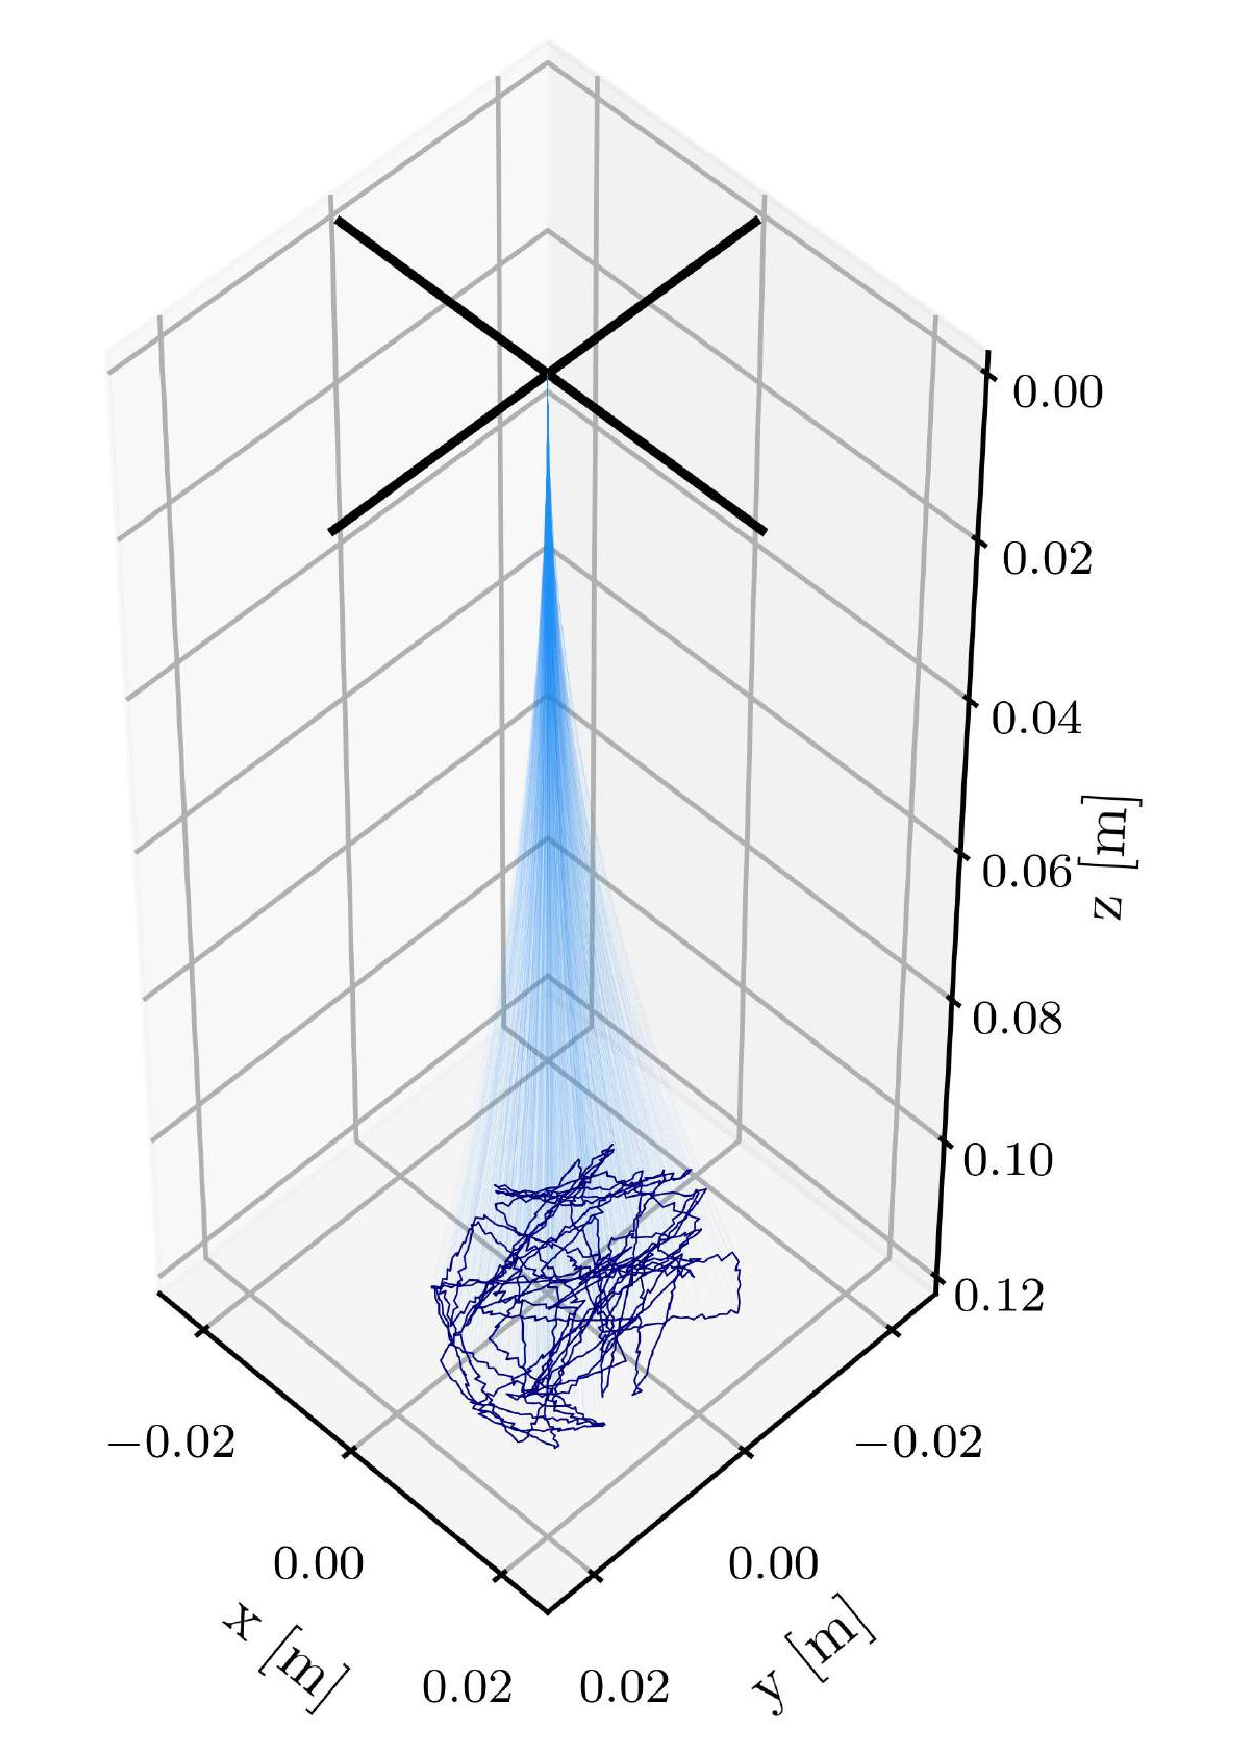
\includegraphics[width=0.16\textwidth]{promasens/figures/trajectories/trajectory_visualizations/random_compressed.pdf}}
  % \hfill% or \hspace{5mm} or \hspace{0.3\textwidth}
  \subfigure[\textbf{T1:} 1D bending]{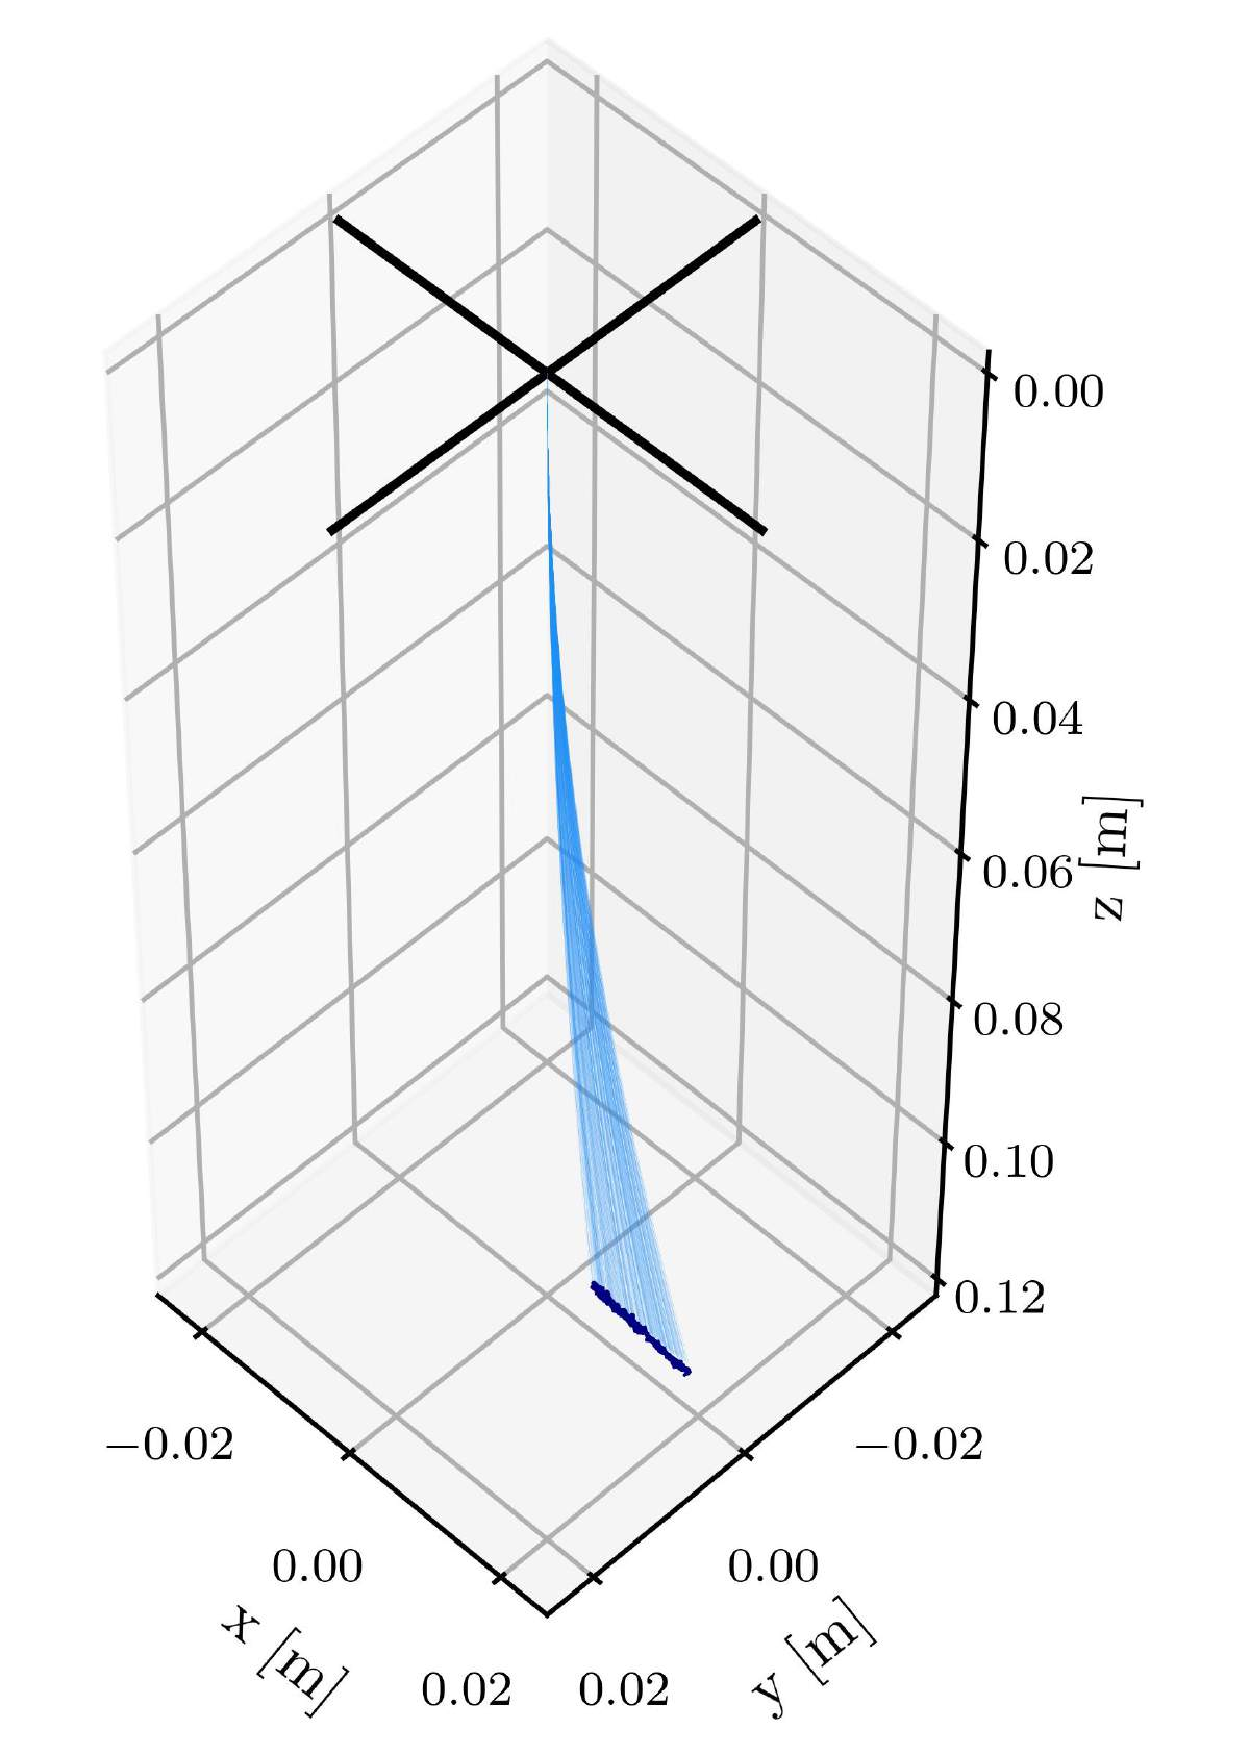
\includegraphics[width=0.16\textwidth]{promasens/figures/trajectories/trajectory_visualizations/1D_bending_compressed.pdf}}
  \subfigure[\textbf{T2:} half lemniscate]{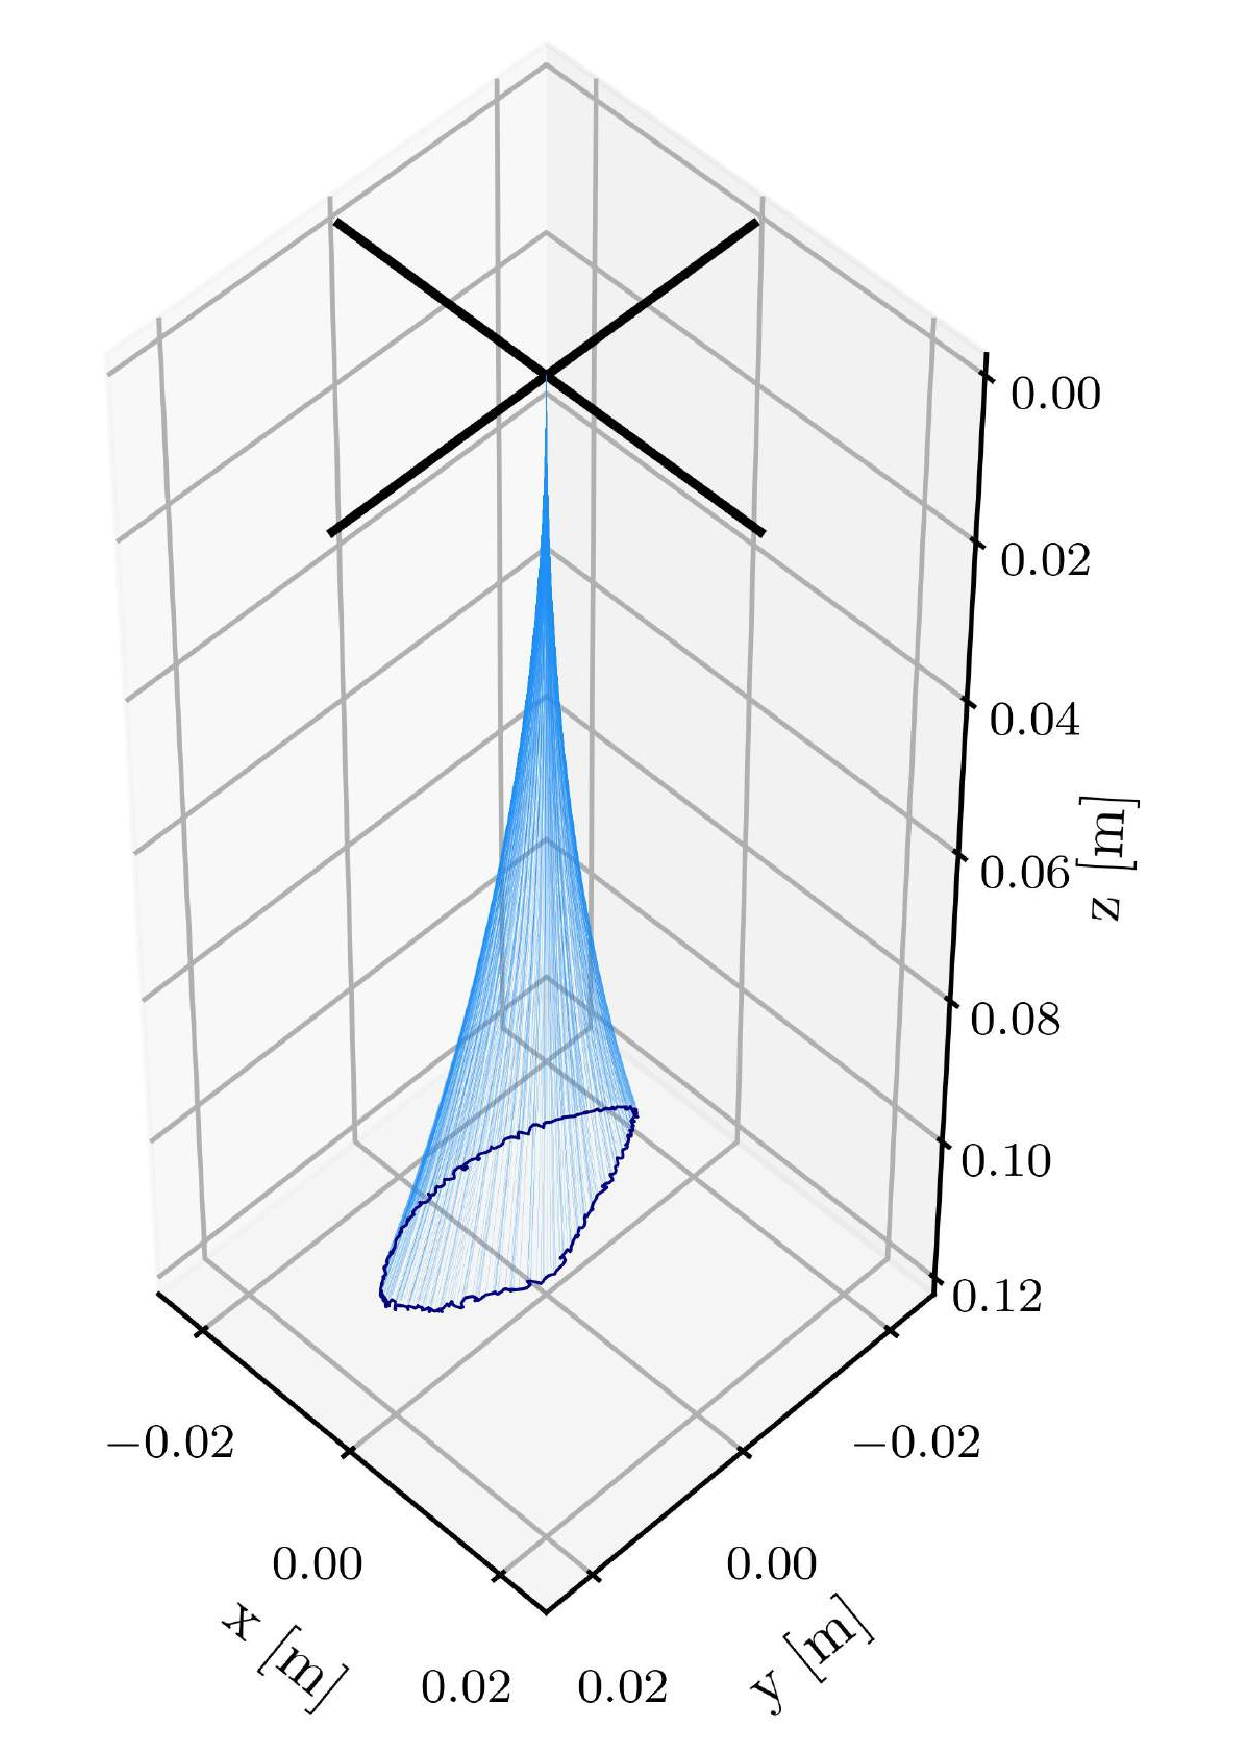
\includegraphics[width=0.16\textwidth]{promasens/figures/trajectories/trajectory_visualizations/half_lemniscate_compressed.pdf}}
  \subfigure[\textbf{T3:} full lemniscate]{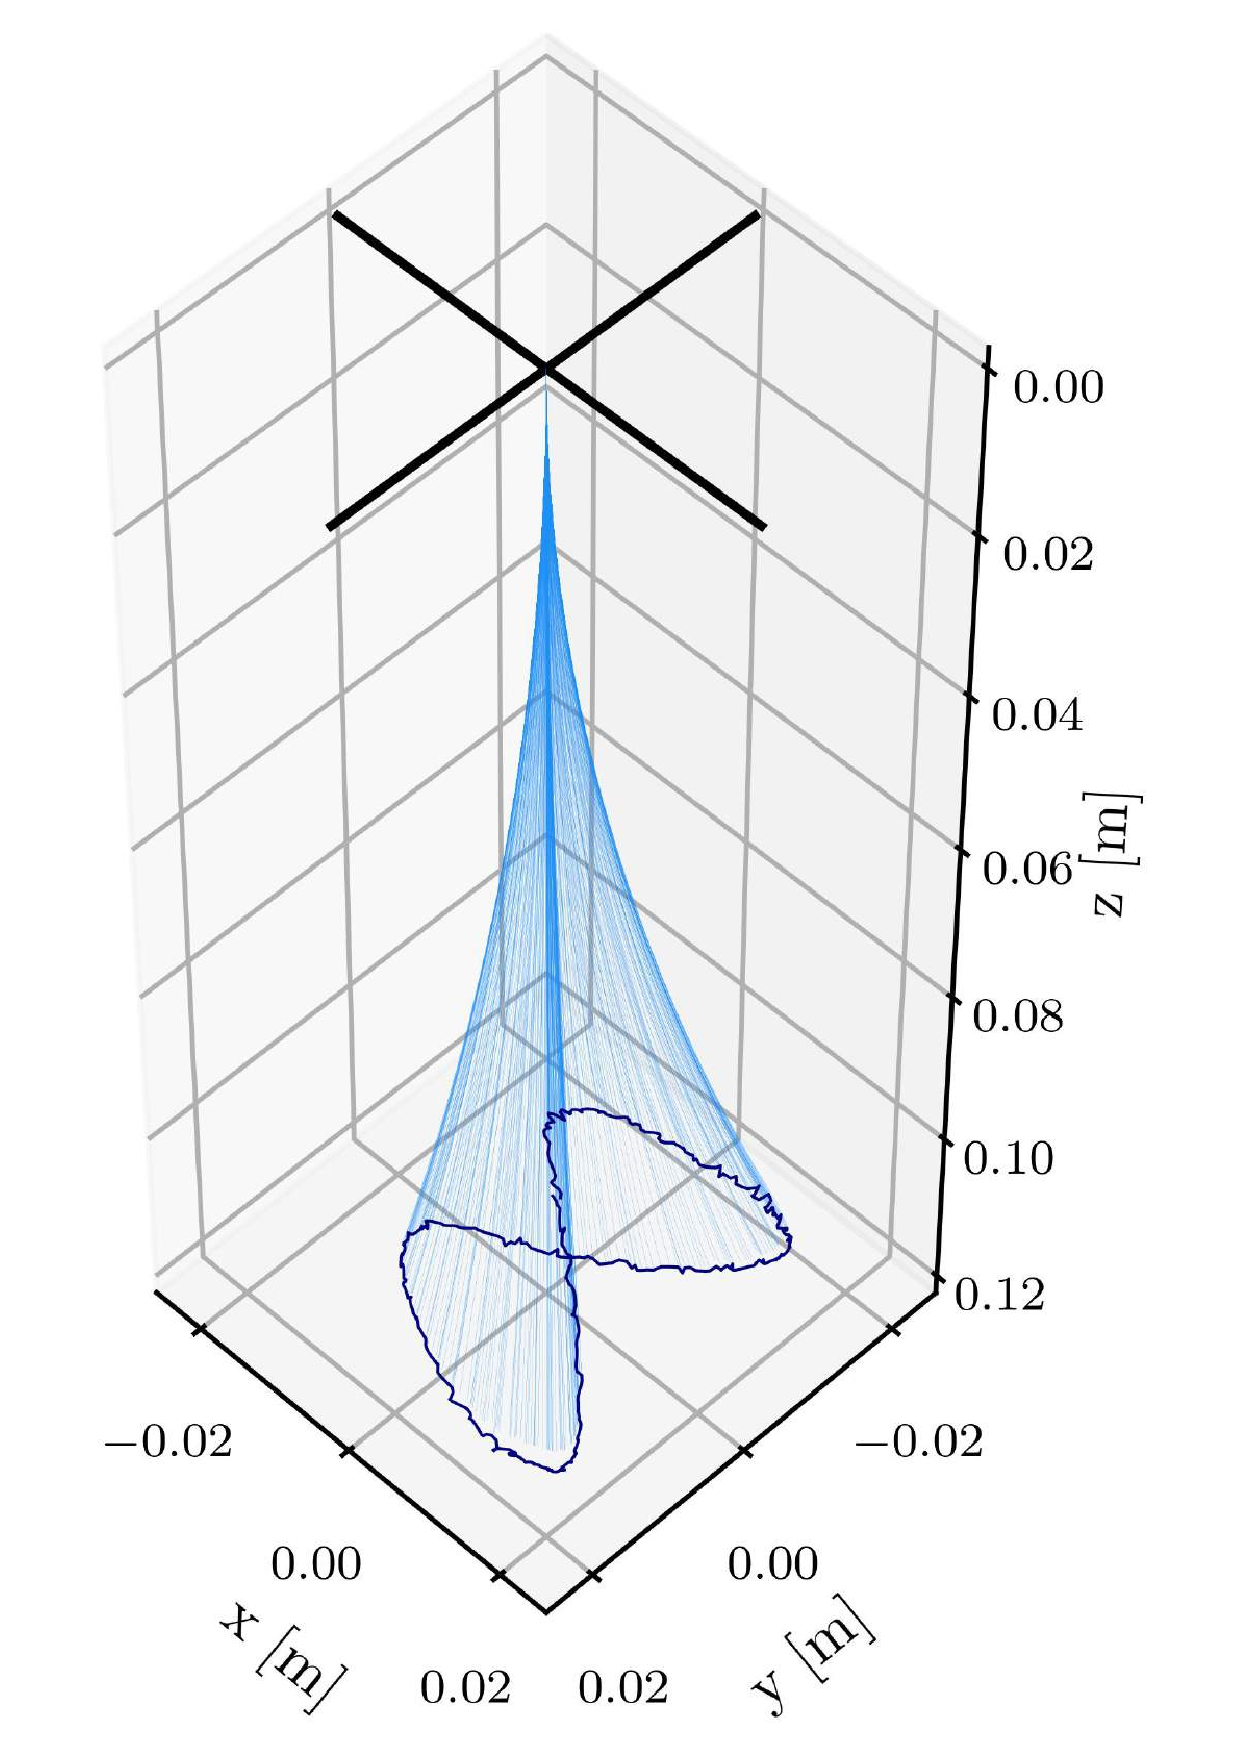
\includegraphics[width=0.16\textwidth]{promasens/figures/trajectories/trajectory_visualizations/full_lemniscate_compressed.pdf}\label{fig:promasens:t3_viz}}
  \subfigure[\textbf{T4:} spiral]{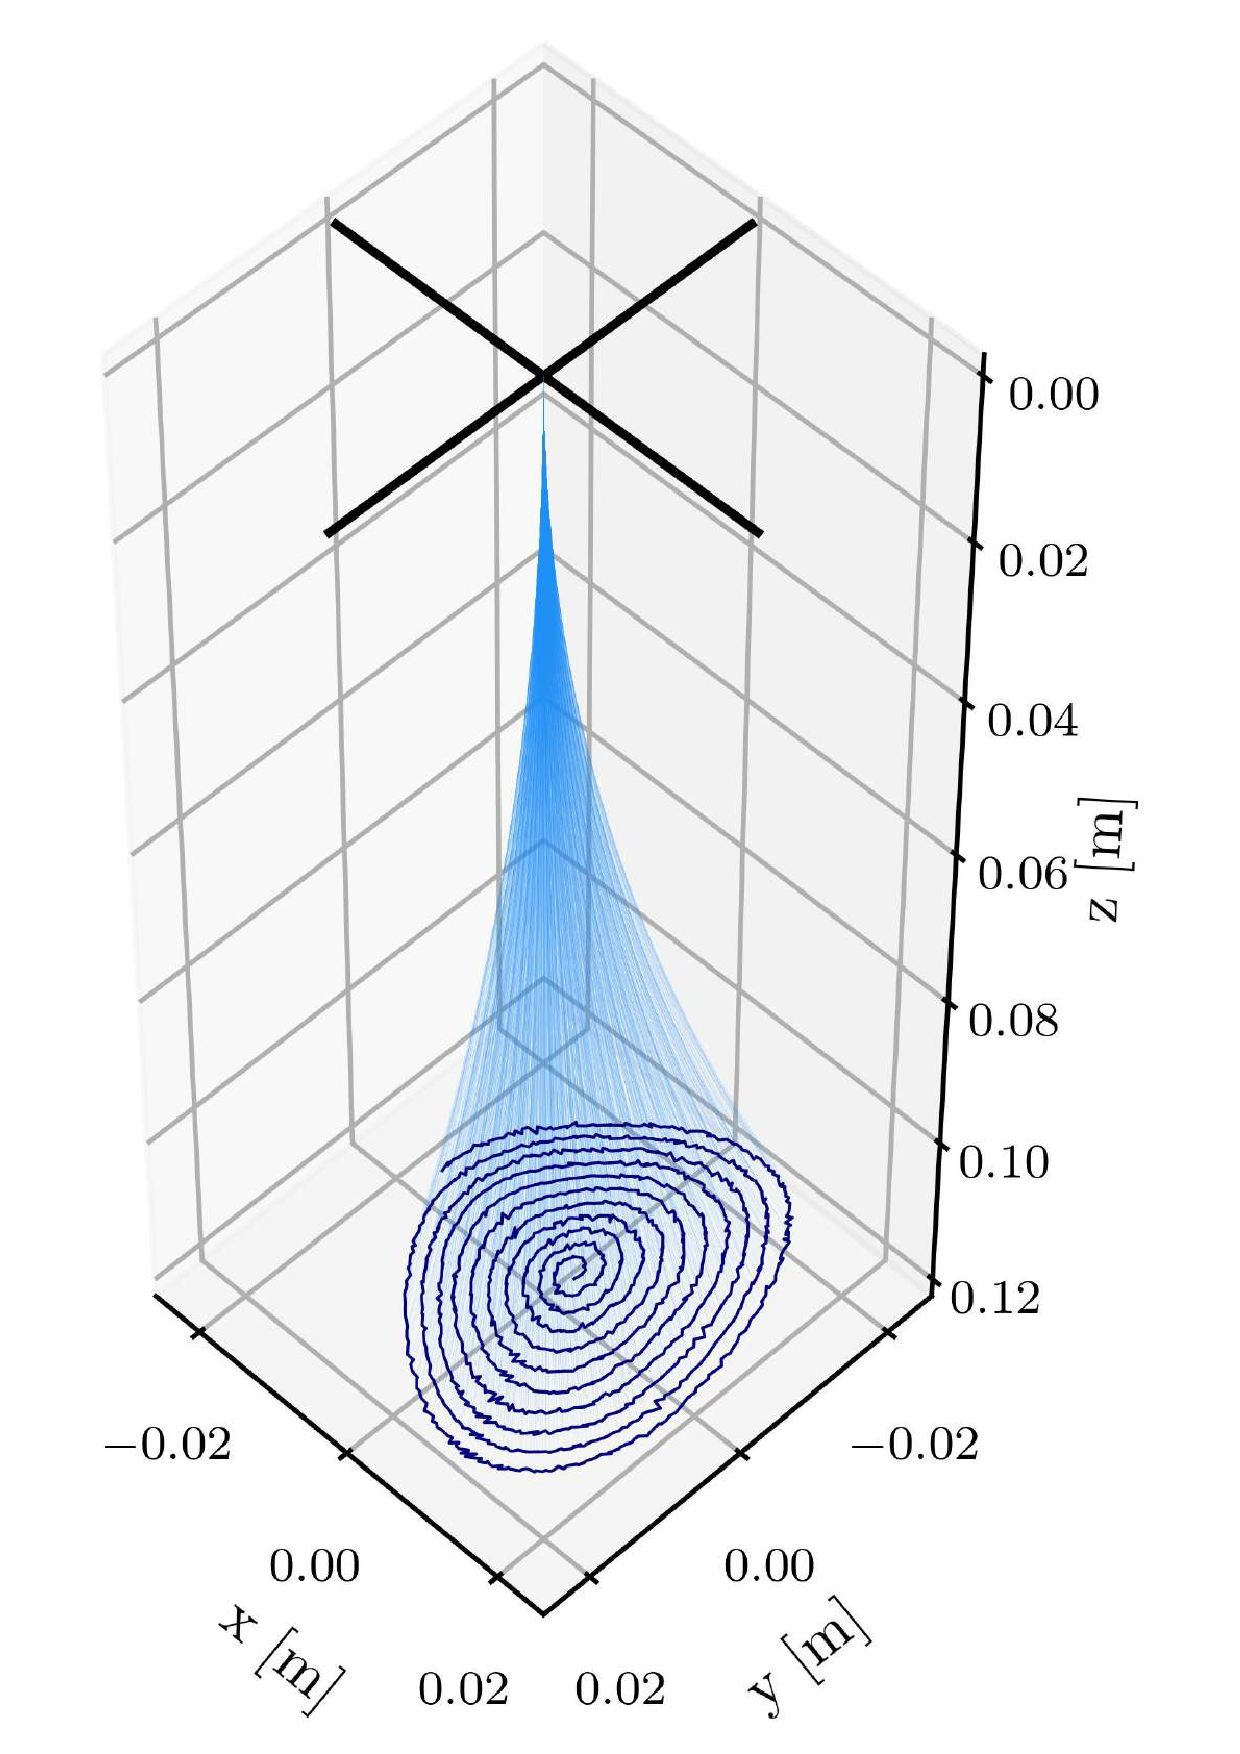
\includegraphics[width=0.16\textwidth]{promasens/figures/trajectories/trajectory_visualizations/spiral_compressed.pdf}}
  \subfigure[\textbf{T5:} flower]{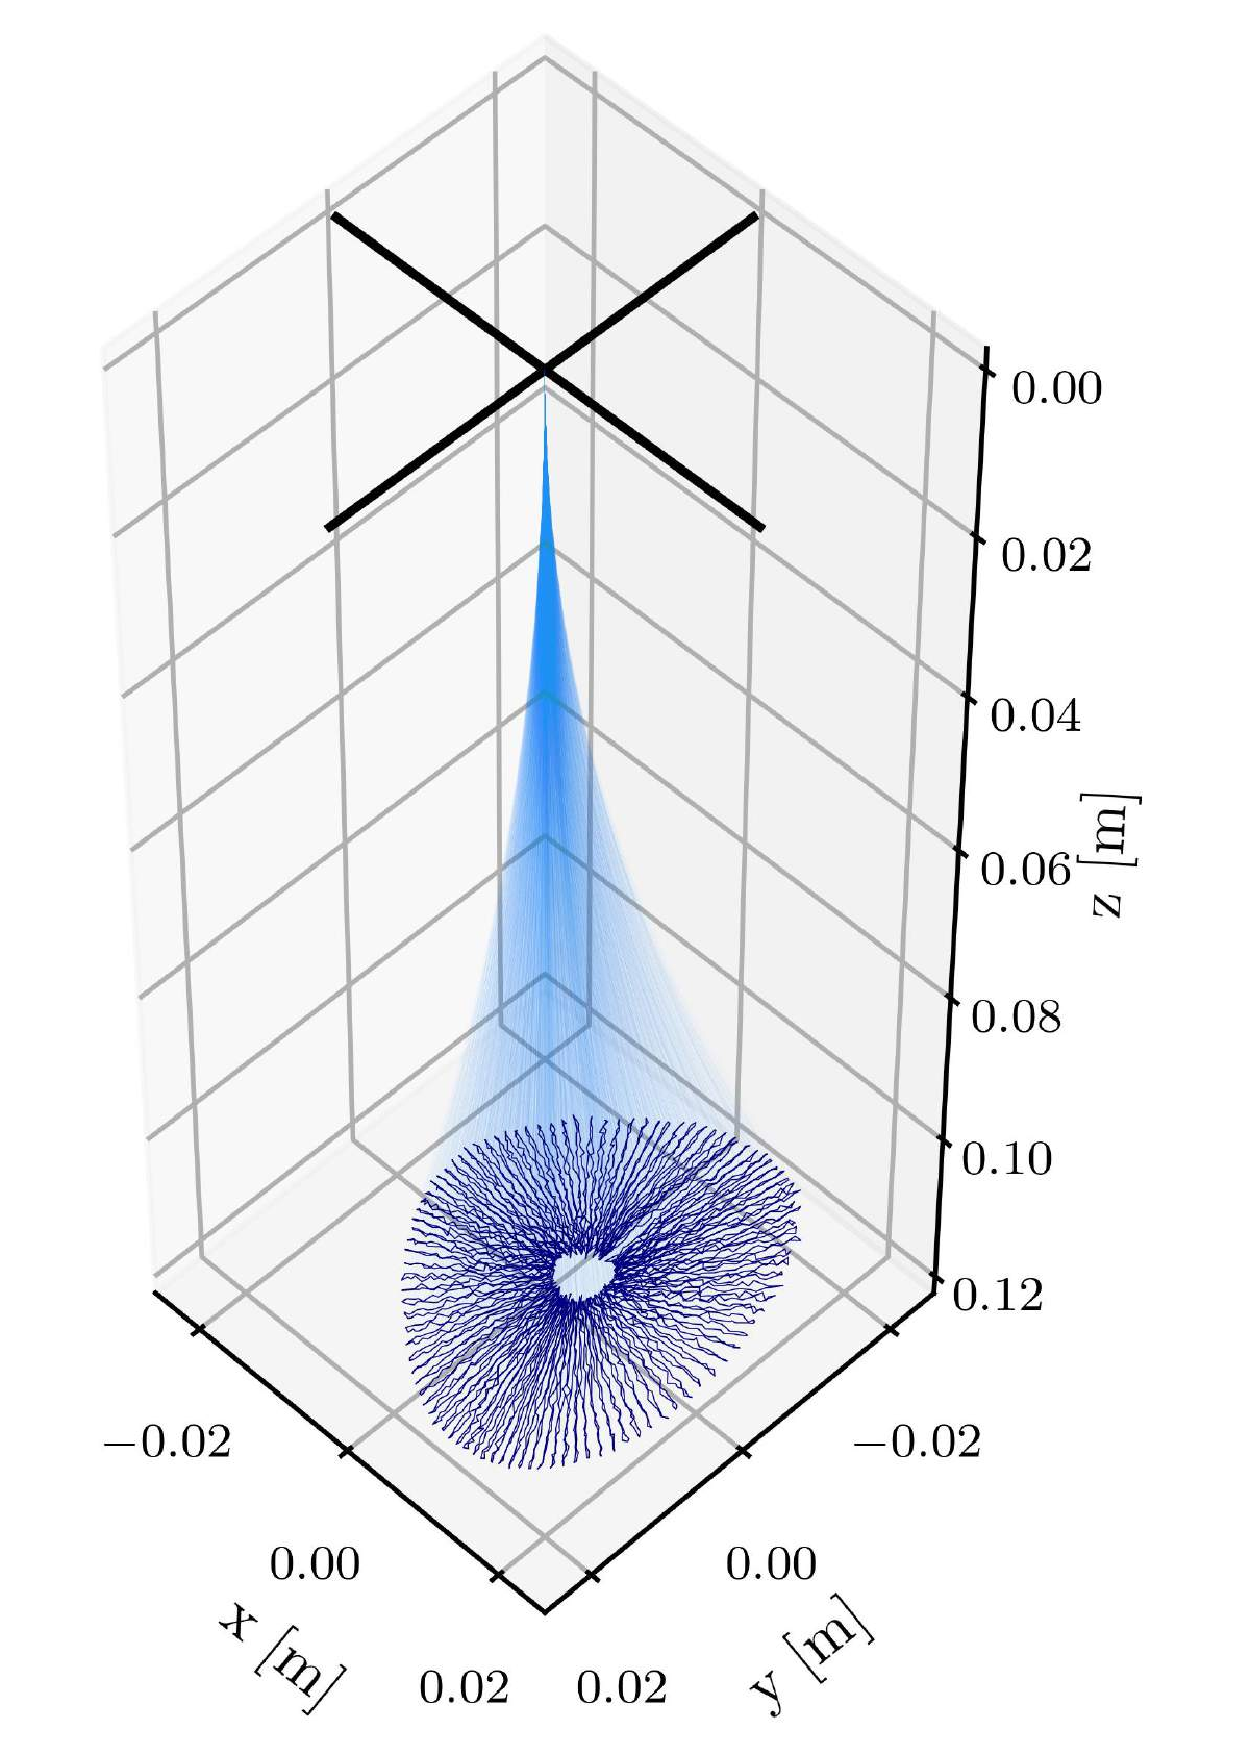
\includegraphics[width=0.16\textwidth]{promasens/figures/trajectories/trajectory_visualizations/flower_compressed.pdf}}
%   \hfill
%   \subfigure[Neural network architecture]{\includegraphics[width=0.33\textwidth]{promasens/figures/Experiments/NN_architecture_P.pdf}\label{fig:promasens:NNgradientdescent}}
  \caption{Trajectories used during the experiments. We plot the shape of the segment under \gls{PCC} approximation in light blue and the position of the tip of the segment in dark blue. 
  % Trajectory 1 represents a 1D bending, trajectory 2 a half lemniscate, trajectory 3 a full lemniscate movement of the tip and trajectory 4 resembles a spiral. 
  % \textbf{Panel (e):} Architecture of the sensor measurement prediction network. Each block consists of a linear layer, a \gls{ReLU}, and a batch norm layer.
  }
  \label{fig:promasens:trajectories}
\end{figure*}

\subsection{Robot design}\label{sub:promasens:robot_design}
We use a cylindrical, pneumatically-actuated soft robotic silicon segment of length $L_{0}=\SI{110}{mm}$ and radius $d_1 = \SI{22}{mm}$ consisting of three independently inflatable cavities evenly spaced in the radial direction from the center line~\cite{marchese2015recipe}. 
% The robot is pneumatically actuated by adjusting the air pressure in each chamber to make the end-effector bend in 3D Cartesian space.
%
The proprioceptive sensing system is achieved by embedding one ring magnet in the backbone at a distance $d_{\mathrm{m}_0} = \SI{55}{mm}$ from the base of the segment and three symmetrically-placed Magnetoresistive Sensors (MRSs) at the tip of the segment as visualized in Fig.~\ref{fig:promasens:experimental_setup}. % Fig.~\ref{fig:promasens:exploded_rendering}.
Although we use MRSs in our experimental setup for their high sensitivity~\cite{popovic2002bridging}, this is not a strict condition and other sensor types measuring the magnetic field such as Hall-effect sensors can be combined with the methodology proposed in this chapter too.
For casting the silicone segment, we use a 3D-printed mold with a holder for the magnet which keeps it in place inside the segment.
The magnet used is a neodymium ring of grade N50 with a thickness and inner diameter of \SI{6}{mm} each, and an outer diameter of \SI{12}{mm}.
%
The MRSs of type Honeywell HMC1021Z are integrated into a Printed Circuit Board (PCB) and output a voltage difference of \SI{50}{mV \per mT}. % ~\cite{honeywell}. 
The three sensors are equally spaced at \SI{120}{\degree} from each other and are placed at a radial distance of $d_{\mathrm{s},\mathrm{r}} = \SI{13}{mm}$, and at a longitudinal distance of $d_{\mathrm{s},\mathrm{a}} = \SI{116}{mm}$ from the base in a straight configuration.
For each sensor, we implemented a Set / Reset and an amplification circuit on the PCB.
The Set / Reset circuit is used for calibration of the sensor by re-aligning the magnetic domains. After amplification of the sensor output by a factor of 100, the output of the sensors is processed with a Texas Instruments ADS1115 module %~\cite{ADS1115module}
resulting in a digital signal of \SI{16}{bit} resolution. All sensor measurements $u$ are in the range $[\SI{0}{mV}, \SI{2048}{mV}]$, which corresponds to magnetic flux densities of  $[\SI{0}{mT}, \SI{41}{mT}]$.

%The \gls{MRS} are mounted on a \gls{PCB} at the tip of the silicone body, with three sensors on one PCB. The exact placement of the sensors is shown in Table \ref{tab:sensor_locations}. The sensors are Honeywell HMC1021Z sensors that have an ideal operating range of $\SI{\pm 6}{Gs}$. The sensor gives a voltage difference of \SI{5}{mV \per Gs} as an output \cite{honeywell,farnell}.
%
% The \gls{PCB} is mounted on either side of the silicone body. The holes in the \gls{PCB} are for the air supply hoses, cables, and mounting. The \gls{PCB} not only contains the sensors, but also the sensor circuitry. Each sensor has its own circuitry containing a Set/Reset circuit and an amplification circuit. The Set/Reset circuit produces a current peak of \SI{1}{A} of duration $\SI{2}{\micro \second}$ for a Set/Reset pulse to calibrate the sensor by realigning the magnetic domains in the sensor in one direction. The amplification circuit amplifies the sensor output by a factor of 100. The output of the sensors is processed with a Texas Instruments ADS1115 module \cite{ADS1115module}. This module reads out the sensor signal in 16 bits and fits it into a format so that the Arduino can read it out. This gives a more precise sensor readout than using the Arduino directly which would only give a \SI{10}{bit} resolution.\\

% Fabrication
% The fabrication process of the silicone body starts by making three wax inserts by pouring beeswax into a silicone mold. Once hardened, these wax inserts are removed from their silicone mold and placed into a 3D-printed mold together with the magnet holder. The magnet holder is a 3D-printed ring that houses the magnet. Subsequently, Dragon Skin 30 silicone is mixed, degassed, and poured into the 3D-printed mold. After hardening, the silicone body, wherein the magnet holder and magnet are embedded, is removed from the mold. Then the wax inserts are melted, leaving three inflatable chambers behind.

% \begin{figure}[ht]
% \centering
% \includegraphics[width=50mm]{promasens/figures/PCB_3d_view_2.png}
% \caption{\gls{PCB} for three \gls{MRS} including Set/Reset circuit to be mounted at the base and tip of each segment.}\label{fig:promasens:PCB}
% \end{figure}
        

\begingroup
\setlength{\tabcolsep}{6pt} % Default value: 6pt
\begin{table*}\footnotesize
\centering
\caption{Experimental results: absolute [mm] and relative RMSE [\%] of sensor measurement predictions and robot configuration estimates for various trajectories. The RMSE is normalized with the range of the dataset for $u$ and each configuration variable respectively as stated in \eqref{eq:promasens:relative_RMSE}. We report the error as $\text{mean} \pm \text{stdev}$ and compute the statistics over three different random seeds. The random seed determines at the start of the training the initialization of the neural network weights.}
\begin{tabular}{l rr rrrr}\toprule
\textbf{Trajectory} & $e_{u}$ [mV] & $e_{u}$ [\%] & $e_{\Delta_x}$ [mm] & $e_{\Delta_x}$ [\%] & $e_{\Delta_y}$ [mm] & $e_{\Delta_y}$ [\%]\\
\midrule
T5.train $\rightarrow$ T0.test & $9.90 \pm 0.90$ & $3.90 \pm 0.40$ & $0.37 \pm 0.06$ & $3.70 \pm 0.60$ & $0.44 \pm 0.01$ & $3.50 \pm 0.10$\\ % T5.slow_to_T0.200mBar
T5.train $\rightarrow$ T1.test & $8.80 \pm 0.30$ & $4.40 \pm 0.10$ & $0.36 \pm 0.08$ & $6.50 \pm 1.50$ & $0.43 \pm 0.05$ & -\\ % T5.slow_to_T1.270
T5.train $\rightarrow$ T2.test & $11.10 \pm 0.30$ & $4.30 \pm 0.10$ & $0.78 \pm 0.03$ & $13.60 \pm 0.60$ & $0.74 \pm 0.23$ & $5.90 \pm 1.80$\\ % T5.slow_to_T2
T5.train $\rightarrow$ T3.test & $12.30 \pm 0.30$ & $4.60 \pm 0.10$ & $0.52 \pm 0.06$ & $4.50 \pm 0.50$ & $0.47 \pm 0.03$ & $3.10 \pm 0.20$\\ % T5.slow_to_T3_90deg
T5.train $\rightarrow$ T4 & $3.01 \pm 0.05$ & $1.08 \pm 0.02$ & $0.33 \pm 0.02$ & $2.40 \pm 0.10$ & $0.52 \pm 0.06$ & $3.10 \pm 0.40$\\ % T5.slow_to_T4.slow.forw
T5.train $\rightarrow$ T5.test & $1.60 \pm 0.10$ & $0.58 \pm 0.05$ & $0.24 \pm 0.05$ & $1.90 \pm 0.30$ & $0.24 \pm 0.01$ & $1.40 \pm 0.05$\\ % T5.slow_to_T5.slow
\bottomrule
\end{tabular}
\label{tab:results_experiments}
\end{table*}
\endgroup

\subsection{Experimental setup}
We conducted our experiments in a lab environment with the base of the soft robot segment mounted in a tip-down configuration to a cubical cage as shown in Figure~\ref{fig:promasens:experimental_setup}.
% Motion Capture System
A 3D-printed ring with four reflective markers is mounted on the tip of the segment.
% Prime X by Optitrack
Eight motion capture cameras are attached to the cage tracking at \SI{40}{Hz} the 3D pose of the ring.
We transform the pose measurements of the tip to the base frame of the robot and compute the closed-form inverse kinematics~\cite{della2020improved} to receive a ground-truth configuration estimate $q(t) \in \mathbb{R}^2$.
% Pneumatic actuation
Each of the three pneumatic chambers of the segment is connected via tubing to a separate valve of a proportional pressure regulator operated at \SI{100}{Hz}. % We send set-point pressure commands from the workstation to the pressure regulator via Modbus / TCP at \SI{100}{Hz}.
% Reading sensor measurements
We read out the analog signals of the magnetoresistive sensors with an Arduino Uno at \SI{40}{Hz} and save them for later offline processing. 
We temporally align the motion capture and the magnetic sensor data by detecting the initial extension of the robot with a suitable threshold.
%static distortion
The sensor noise is determined for both an unelongated straight configuration, and during fully inflated bending. Here the standard deviations of the white noise are \SI{0.24}{mV} and \SI{3.55}{mV}, which normalizes to \SI{0.03}{\percent} and \SI{2}{\percent} of the dynamic range respectively.
% earth's magnetic field
% Furthermore, we measure the angle between the x-axis of the base frame and the magnetic north with a compass as $\varphi_\mathrm{e} = \SI{3.79}{\radian}$ and rely on the \gls{WMM}~\cite{chulliat2020us} to identify the vertical component of the earth's magnetic field. This results in a unit vector for the earth's magnetic field direction of $\{ \hat{n}_{\mathrm{e}} \}_{0} = (-0.311, -0.234, 0.921)^\mathrm{T}$ for the robot in tip-down configuration.
Furthermore, we identify the earth's magnetic field direction in the base from as $\{ \hat{n}_{\mathrm{e}} \}_{0} = (-0.311, -0.234, 0.921)^\mathrm{T}$ using a compass and the World Magnetic Model (WMM)~\cite{chulliat2020us}.

\begin{figure*}[hbt]
  \centering
  \subfigure[Loss landscape]{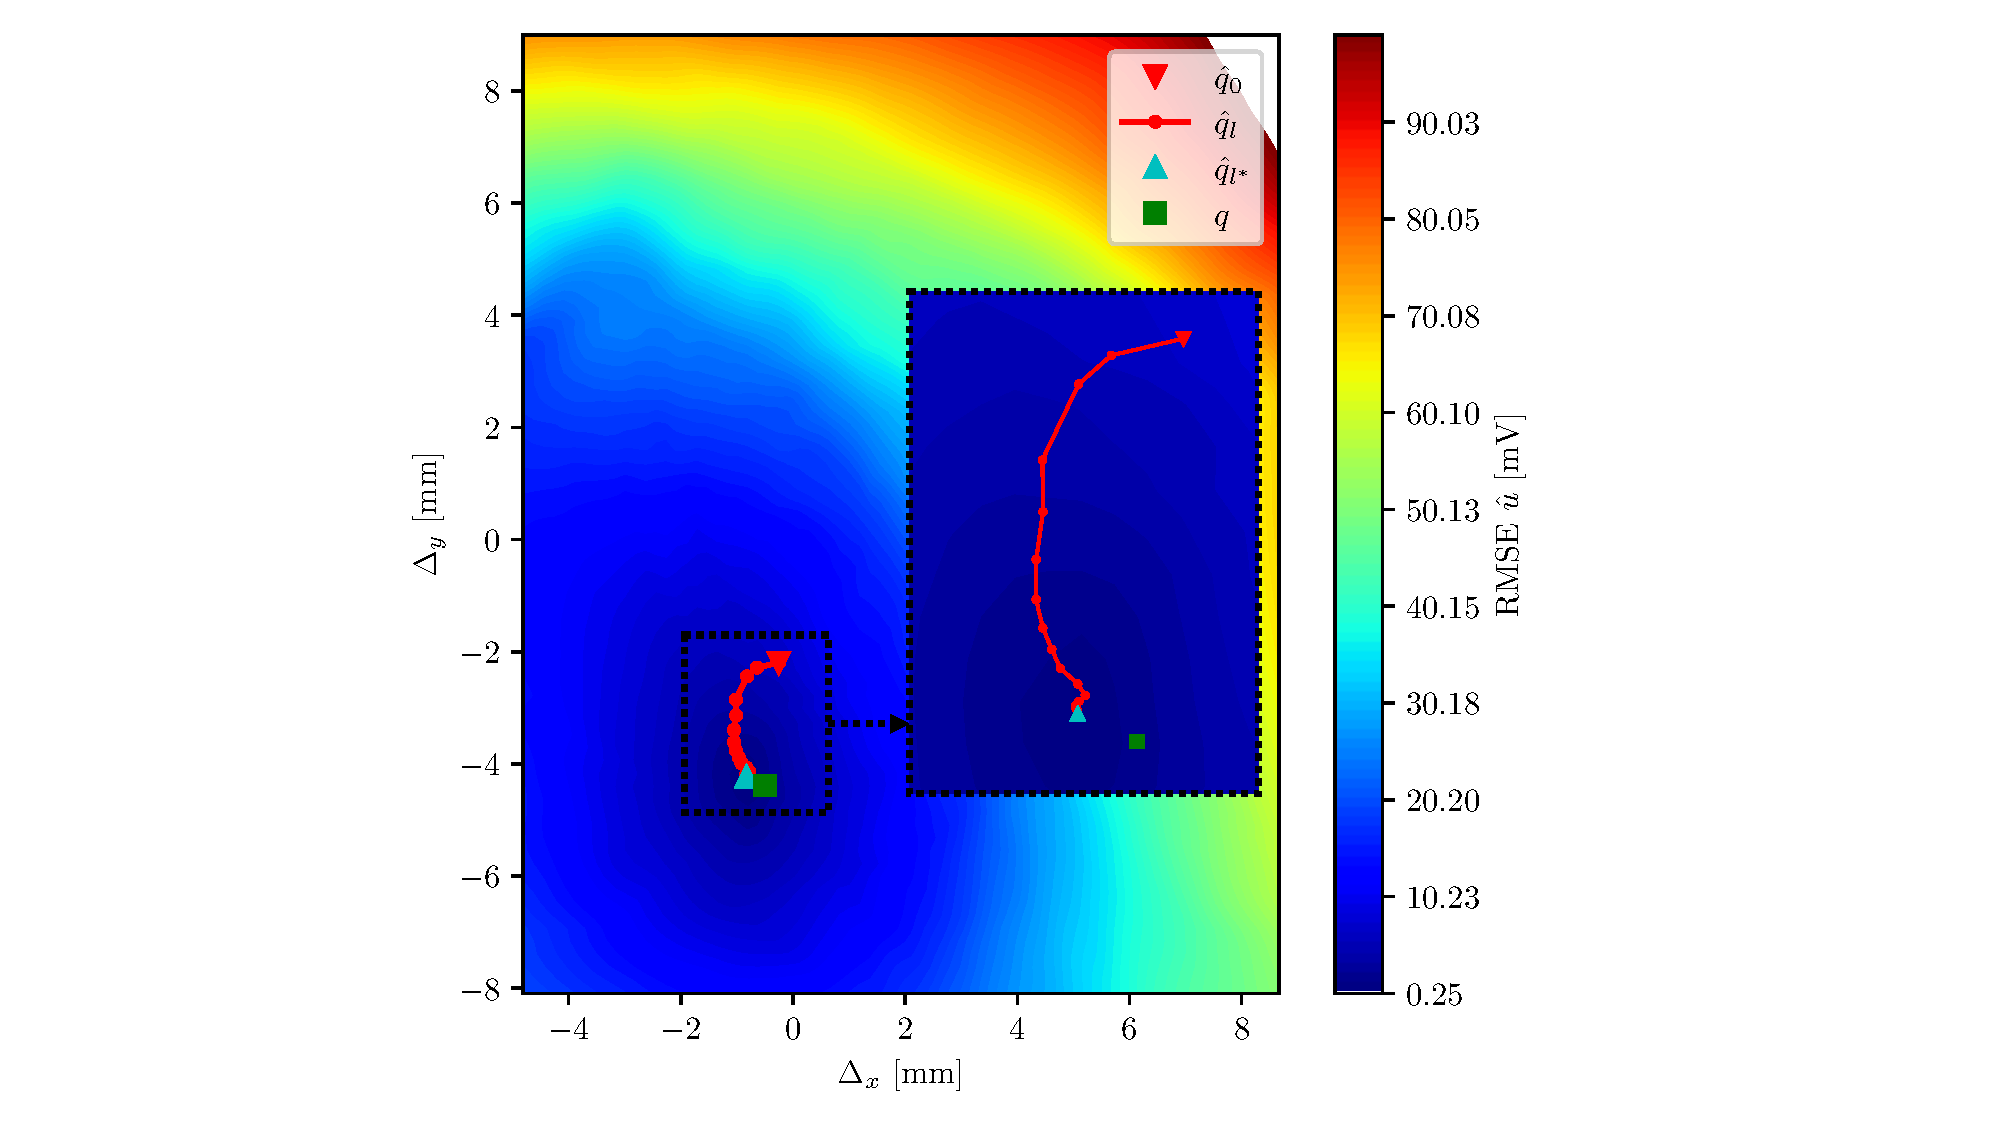
\includegraphics[width=0.3125\textwidth]{promasens/figures/loss_landscape/loss_landscape_v3_cropped.pdf}\label{fig:promasens:loss_landscape}}
  %
  \subfigure[Experimental results for T2 (top) and T5 (bottom)]{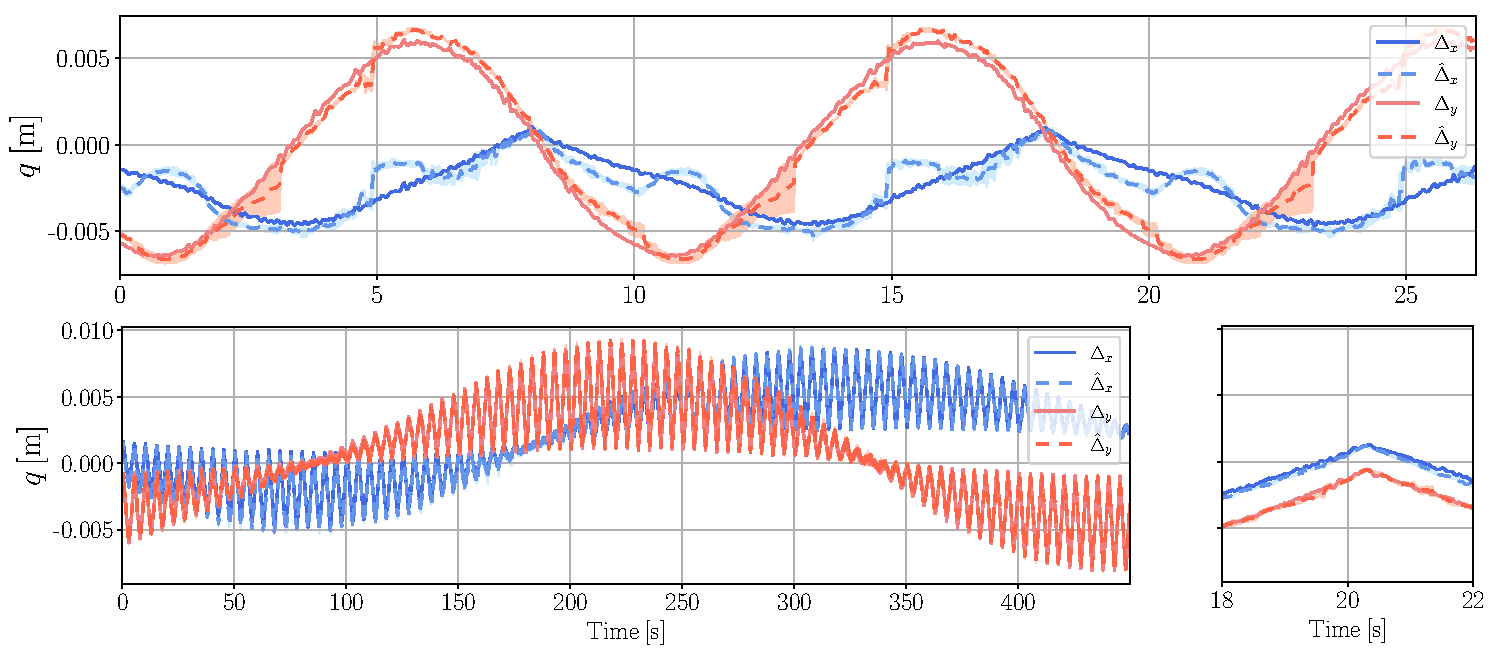
\includegraphics[width=0.6775\textwidth]{promasens/figures/experimental_results/2022-05-02_results_merged.pdf}\label{fig:promasens:2022-05-02_results_merged}}\\ %  [T5.train $\rightarrow$ T2.test] [T5.train $\rightarrow$ T5.test]
  
  \caption{\textbf{Panel (a):} Sample loss landscape for optimization of $\Delta_x$ and $\Delta_y$ on T5. With the hue, we visualize the RMSE of the sensor measurement prediction $\hat{u}$ for a given configuration $\hat{q} = (\Delta_x, \Delta_y)^\mathrm{T}$. Additionally, we denote the initial configuration estimate with $\hat{q}_0$, the trajectory of the gradient descent with $\hat{q}_l$, the optimal configuration with $\hat{q}$, and the ground truth with $q$. \textbf{Panel (b) top:} Proprioception on the test set of T2 using a model trained on T5. \textbf{Panel (b) bottom:} Configuration estimates for a model trained and evaluated on separated parts of trajectory 5. We plot the ground-truth configuration $q$ in solid, the estimate $\hat{q}$ as a mean over three random seeds with dashed lines, and the standard deviation as an error band. The bottom right plot zooms onto a selected part of T5 (e.g. \SI{18}{s} to \SI{22}{s}) to more clearly visually distinguish the dashed lines from the solid lines.}
  \label{fig:promasens:results_trajectories}
\end{figure*}

\subsection{Pneumatic actuation and trajectories}
% We consider two actuation sequence types in this chapter: a) a randomized actuation sequence consisting of steps generated with \gls{GBN}~\cite{tulleken1990generalized} primarily used for training and b) three continuous trajectories consisting of planar side bending, and the tip following half-8-shape and full 8-shapes as plotted in Fig.~\ref{fig:promasens:trajectories}.
We consider, as visualized in Fig.~\ref{fig:promasens:trajectories}, six continuous actuation sequences in this chapter: random configuration way-points which are connected through linear interpolation (T0), planar side bending (T1), the tip following a half lemniscate (T2) and full lemniscate (T3), a spiral with constant linear velocity~\cite{carrasco2018constant} (T4) and finally a flower-shape (T5).
We define our trajectories as wrenches  $\tau_\mathrm{xyz} = \begin{bmatrix} \tau_\mathrm{x} & \tau_\mathrm{y} \end{bmatrix}^\mathrm{T}$ on the tip of the segment in Cartesian space, where $\tau_\mathrm{x}$ and $\tau_\mathrm{y}$ cause bending around the local x- and y-axis  of the tip respectively. % $f_\mathrm{z}$ is a force leading the segment to extend uniformly.
The pressures we command from the pressure regulator are given by inversely evaluating the force produced at the center of pressure at the tip of the segment for each chamber for a given chamber pressure~\cite{della2019dynamic}.
All actuation sequences are preceded by first applying an offset pressure of \SI{225}{mBar} in all chambers, which causes a near-constant elongation of the segment. The peak pressure, which causes maximum bending, is set for all trajectories to \SI{450}{mBar}.

% The \gls{GBN}~\cite{tulleken1990generalized} algorithm with an expected settling time of \SI{5}{s} determines the timing of when we command a step to a new random wrench $\tau_{xzy}$.
% We uniformly sample a bending azimuth angle $\varphi \sim \mathcal{U}\left(0, 2 \pi\right)$, a bending torque magnitude $|\tau| \sim \mathcal{U}\left(0, \tau_\mathrm{max}\right)$ and accordingly compute $\tau_\mathrm{xyz}$ as
% \begin{equation}
%     \tau_\mathrm{x} = \cos(\varphi) |\tau| \qquad \tau_\mathrm{y} = \sin(\varphi) |\tau|
% \end{equation}
% and set $f_\mathrm{z}$ to a constant force with corresponding symmetric pressure of \SI{200}{mBar} in the chambers. The maximum bending torque $\tau_\mathrm{max}$ corresponds to a peak pressure in the chambers of \SI{425}{mBar}

% The planar side bending, half lemniscate, and full lemniscate trajectories are generated with a recurring linear torque increase/decrease sequence up to a peak pressure of \SI{425}{mBar}.
% Each T1-T3 trajectory is repeated six times to extend the length of the dataset.
% The spiral trajectory consists of linearly increasing the torque amplitude from a peak pressure of \SI{305}{mBar} to \SI{425}{mBar} over a duration of \SI{110}{s} while at the same time tracking a circular motion with an angular velocity of \SI{1.26}{rad/s}. In the second half of the trajectory, which is later used as a test set, the peak pressure is accordingly linearly decreased over time.

%The spiral trajectory consists of linearly increasing the torque amplitude from a peak pressure of \SI{305}{mBar} to \SI{425}{mBar} over a duration of \SI{110}{s} while at the same time tracking a circular motion with an angular velocity of \SI{1.26}{rad/s}. In the second half of the trajectory, which is later used as a test set, the peak pressure is accordingly linearly decreased over time. 

%The first part is generated with
%\begin{equation}
%    \tau_\mathrm{x} = \frac{2 t}{n_\mathrm{t}} \sin(2 \pi f t) \,     \tau_\mathrm{max} \qquad \tau_\mathrm{y} = \frac{2        t}{n_\mathrm{t}} \sin(2 \pi f t) \, \tau_\mathrm{max},
%\end{equation}
%where $f=\SI{0.2}{Hz}$ represents the frequency, and $\tau_\mathrm{max}$ the peak bending torque of the trajectory with a corresponding peak pressure of \SI{410}{mBar} in the chambers. We denote with $t$ the time and $n_\mathrm{t}$ the duration of the trajectory.

%Very similarly, we generate the planar side bending, half-8-shape, and full-8-shape trajectories with a recurring linear torque increase/decrease sequence up to a peak pressure of \SI{410}{mBar}.
%Each T1-T3 trajectory is repeated six times to extend the length of the dataset.

% We generate the planar side bending, half-8-shape, and full 8-shape trajectories with the following function:
% \begin{equation}
%     \tau_\mathrm{x} = A_x \sin(2 \pi F_x f t) \tau_\mathrm{max} \qquad \tau_\mathrm{y} = A_y \sin(2 \pi F_y f t) \tau_\mathrm{max}
% \end{equation}
% with an offset pressure of \SI{200}{mBar} causing a constant extension of the segment, $f$ representing the trajectory frequency, $\tau_\mathrm{max}$ the peak bending torque of the trajectory with a corresponding peak pressure of \SI{410}{mBar} in the chambers and $t$ the trajectory time.
% Duration of $n_\mathrm{t}=\SI{3.8}{s}$
% \textcolor{red}{TODO: fix this}
% We choose $F_x$, $F_y$, $A_x$, and $A_y$ appropriately to generate the different trajectories, which we report in Tab.~\ref{tab:trajectory_params}.

The 1D bending (T1), half lemniscate (T2) and full lemniscate (T3) are all executed periodically with a period of \SI{5}{s}, \SI{10}{s}, and \SI{10}{s} respectively. 
Trajectories T0 and T4 are characterized by a constant velocity in torque-space of \SI{0.025}{Nm \per s} and \SI{0.0125}{kNm \per s} respectively.
The flower trajectory T5 can be described as periodic 1D bending with a linearly changing azimuth angle. It exhibits an angular velocity of \SI{0.0126}{rad \per s} and a period of \SI{10}{s} for the bending, which results in $50$ bending cycles per circumnavigation.
While the random configuration setpoints of T0 are recorded for \SI{200}{s}, T1, T2 and T3 have total a duration of \SI{90}{s} each, and the spiral T4 and flower T5 last for \SI{120}{s} and \SI{1500}{s} respectively.
We split off the final \SI{20}{\percent} of all datasets as a test set.


% \begin{figure*}[ht]
%     \centering
%     \scalebox{0.5}{
%     \begin{tabular}{llllllllll}
%     \includegraphics[width=0.15\linewidth]{promasens/figures/Experiments/T1F/T1Fscene00001.png} &
%     \includegraphics[width=0.15\linewidth]{promasens/figures/Experiments/T1F/T1Fscene00031.png} &
%     \includegraphics[width=0.15\linewidth]{promasens/figures/Experiments/T1F/T1Fscene00061.png} &
%     \includegraphics[width=0.15\linewidth]{promasens/figures/Experiments/T1F/T1Fscene00091.png} &
%     \includegraphics[width=0.15\linewidth]{promasens/figures/Experiments/T1F/T1Fscene00121.png} &
%     \includegraphics[width=0.15\linewidth]{promasens/figures/Experiments/T1F/T1Fscene00151.png} &
%     \includegraphics[width=0.15\linewidth]{promasens/figures/Experiments/T1F/T1Fscene00181.png} &
%     \includegraphics[width=0.15\linewidth]{promasens/figures/Experiments/T1F/T1Fscene00211.png} &
%     \includegraphics[width=0.15\linewidth]{promasens/figures/Experiments/T1F/T1Fscene00301.png} &
%     \includegraphics[width=0.15\linewidth]{promasens/figures/Experiments/T1F/T1Fscene00331.png} \\
%     \includegraphics[width=0.15\linewidth]{promasens/figures/Experiments/T1S/T1Sscene00001.png} &
%     \includegraphics[width=0.15\linewidth]{promasens/figures/Experiments/T1S/T1Sscene00031.png} &
%     \includegraphics[width=0.15\linewidth]{promasens/figures/Experiments/T1S/T1Sscene00061.png} &
%     \includegraphics[width=0.15\linewidth]{promasens/figures/Experiments/T1S/T1Sscene00091.png} &
%     \includegraphics[width=0.15\linewidth]{promasens/figures/Experiments/T1S/T1Sscene00121.png} &
%     \includegraphics[width=0.15\linewidth]{promasens/figures/Experiments/T1S/T1Sscene00151.png} &
%     \includegraphics[width=0.15\linewidth]{promasens/figures/Experiments/T1S/T1Sscene00181.png} &
%     \includegraphics[width=0.15\linewidth]{promasens/figures/Experiments/T1S/T1Sscene00211.png} &
%     \includegraphics[width=0.15\linewidth]{promasens/figures/Experiments/T1S/T1Sscene00301.png} &
%     \includegraphics[width=0.15\linewidth]{promasens/figures/Experiments/T1S/T1Sscene00331.png}
%  \\
%     \end{tabular}}
%     \caption{Trajectory 1: sequence of stills from a front view (top row) and side view (bottom row)}
%     \label{fig:promasens:trajectory_snapshots_T1}
% \end{figure*}

% \begin{figure*}[ht]
%     \centering
%     \scalebox{0.5}{
%     \begin{tabular}{llllllllll}
%     \includegraphics[width=0.15\linewidth]{promasens/figures/Experiments/T2F/T2Fscene00059.png} &
%     \includegraphics[width=0.15\linewidth]{promasens/figures/Experiments/T2F/T2Fscene00088.png} &
%     \includegraphics[width=0.15\linewidth]{promasens/figures/Experiments/T2F/T2Fscene00117.png} &
%     \includegraphics[width=0.15\linewidth]{promasens/figures/Experiments/T2F/T2Fscene00146.png} &
%     \includegraphics[width=0.15\linewidth]{promasens/figures/Experiments/T2F/T2Fscene00175.png} &
%     \includegraphics[width=0.15\linewidth]{promasens/figures/Experiments/T2F/T2Fscene00204.png} &
%     \includegraphics[width=0.15\linewidth]{promasens/figures/Experiments/T2F/T2Fscene00233.png} &
%     \includegraphics[width=0.15\linewidth]{promasens/figures/Experiments/T2F/T2Fscene00262.png} &
%     \includegraphics[width=0.15\linewidth]{promasens/figures/Experiments/T2F/T2Fscene00291.png} &
%     \includegraphics[width=0.15\linewidth]{promasens/figures/Experiments/T2F/T2Fscene00320.png} \\
%     \includegraphics[width=0.15\linewidth]{promasens/figures/Experiments/T2S/T2Sscene00061.png} &
%     \includegraphics[width=0.15\linewidth]{promasens/figures/Experiments/T2S/T2Sscene00061.png} &
%     \includegraphics[width=0.15\linewidth]{promasens/figures/Experiments/T2S/T2Sscene00091.png} &
%     \includegraphics[width=0.15\linewidth]{promasens/figures/Experiments/T2S/T2Sscene00121.png} &
%     \includegraphics[width=0.15\linewidth]{promasens/figures/Experiments/T2S/T2Sscene00151.png} &
%     \includegraphics[width=0.15\linewidth]{promasens/figures/Experiments/T2S/T2Sscene00181.png} &
%     \includegraphics[width=0.15\linewidth]{promasens/figures/Experiments/T2S/T2Sscene00211.png} &
%     \includegraphics[width=0.15\linewidth]{promasens/figures/Experiments/T2S/T2Sscene00241.png} &
%     \includegraphics[width=0.15\linewidth]{promasens/figures/Experiments/T2S/T2Sscene00271.png} &
%     \includegraphics[width=0.15\linewidth]{promasens/figures/Experiments/T2S/T2Sscene00301.png} \\
%  \\
%     \end{tabular}}
%     \caption{Trajectory 2: sequence of stills from a front view (top row) and side view (bottom row)}
%     \label{fig:promasens:trajectory_snapshots_T2}
% \end{figure*}

% \begin{figure*}[ht]
%     \centering
%     \scalebox{0.5}{
%     \begin{tabular}{llllllllll}
%     \includegraphics[width=0.15\linewidth]{promasens/figures/Experiments/T3F/T3Fscene00121.png} &
%     \includegraphics[width=0.15\linewidth]{promasens/figures/Experiments/T3F/T3Fscene00151.png} &
%     \includegraphics[width=0.15\linewidth]{promasens/figures/Experiments/T3F/T3Fscene00181.png} &
%     \includegraphics[width=0.15\linewidth]{promasens/figures/Experiments/T3F/T3Fscene00211.png} &
%     \includegraphics[width=0.15\linewidth]{promasens/figures/Experiments/T3F/T3Fscene00241.png} &
%     \includegraphics[width=0.15\linewidth]{promasens/figures/Experiments/T3F/T3Fscene00271.png} &
%     \includegraphics[width=0.15\linewidth]{promasens/figures/Experiments/T3F/T3Fscene00301.png} &
%     \includegraphics[width=0.15\linewidth]{promasens/figures/Experiments/T3F/T3Fscene00331.png} &
%     \includegraphics[width=0.15\linewidth]{promasens/figures/Experiments/T3F/T3Fscene00361.png} &
%     \includegraphics[width=0.15\linewidth]{promasens/figures/Experiments/T3F/T3Fscene00391.png} \\
%     \includegraphics[width=0.15\linewidth]{promasens/figures/Experiments/T3S/T3Sscene00121.png} &
%     \includegraphics[width=0.15\linewidth]{promasens/figures/Experiments/T3S/T3Sscene00151.png} &
%     \includegraphics[width=0.15\linewidth]{promasens/figures/Experiments/T3S/T3Sscene00181.png} &
%     \includegraphics[width=0.15\linewidth]{promasens/figures/Experiments/T3S/T3Sscene00211.png} &
%     \includegraphics[width=0.15\linewidth]{promasens/figures/Experiments/T3S/T3Sscene00241.png} &
%     \includegraphics[width=0.15\linewidth]{promasens/figures/Experiments/T3S/T3Sscene00271.png} &
%     \includegraphics[width=0.15\linewidth]{promasens/figures/Experiments/T3S/T3Sscene00301.png} &
%     \includegraphics[width=0.15\linewidth]{promasens/figures/Experiments/T3S/T3Sscene00331.png} &
%     \includegraphics[width=0.15\linewidth]{promasens/figures/Experiments/T3S/T3Sscene00361.png} &
%     \includegraphics[width=0.15\linewidth]{promasens/figures/Experiments/T3S/T3Sscene00391.png} \\
%     \end{tabular}}
%     \caption{Trajectory 3: sequence of stills from a front view (top row) and side view (bottom row)}
%     \label{fig:promasens:trajectory_snapshots_T3}
% \end{figure*}

% \begingroup
% \setlength{\tabcolsep}{3.5pt} % Default value: 6pt
% \begin{table*}% 
% \centering
% \caption{Experimental results: absolute and relative \gls{RMSE} of sensor measurement predictions by the neural network. For the relative RMSE, the absolute RMSE is normalized with the range of $u$ on the test set. We report the error as $\text{mean} \pm \text{stdev}$ and compute the statistics over three different random seeds.}
% \begin{tabular}{l cc cc cc}\toprule
% \textbf{Error} & \textbf{T5.train $\rightarrow$ T0.test} & \textbf{T5.train $\rightarrow$ T1.test} & \textbf{T5.train $\rightarrow$ T2.test} & \textbf{T5.train $\rightarrow$ T3.test} & \textbf{T5.train $\rightarrow$ T4} & \textbf{T5.train $\rightarrow$ T5.test} \\
% \midrule
% Abs. RMSE [mV] & $9.9 \pm 0.9$ & $8.8 \pm 0.3$ & $11.1 \pm 0.3$  & $12.3 \pm 0.3$ & $3.01 \pm 0.05$ & $1.6 \pm 0.1$ \\
% Rel. RMSE [\%] & $3.9 \pm 0.4$ & $4.4 \pm 0.1$ & $4.3 \pm 0.1$ & $4.6 \pm 0.1$ & $1.08 \pm 0.02$ & $0.58 \pm 0.05$ \\
% \bottomrule
% \end{tabular}
% \label{tab:results_experiments_sensor_measurement_prediction}
% \end{table*}
% \endgroup

% \begin{figure}[htb]
%     \centering
%     \includegraphics[width=1.0\columnwidth]{promasens/figures/loss_landscape/loss_landscape_v3_cropped.pdf}
%     \caption{Sample loss landscape for optimization of $\Delta_x$ and $\Delta_y$. With the hue, we visualize the RMSE representing the error $\lVert \hat{u} - u(t) \rVert$ for a given $\hat{q}$. Additionally, we denote the trajectory of the gradient descent with $\hat{q}_l$, the optimized configuration with $\hat{q}$, and the ground-truth with $q$.}\label{fig:promasens:loss_landscape}
% \end{figure}

% \begin{figure*}[ht]
%   \centering
%   \hspace{-0.4cm}
%   \subfigure{\includegraphics[width=\textwidth]{promasens/figures/experimental_results/2022-05-02_FLOWER_SLOW_NOMINAL_P0_R1_to_2022-05-02_T2_P0_R1_size_(16.0, 4.0)_cropped.pdf}\label{fig:promasens:results_T5_to_T2}}\\ % [T5.train $\rightarrow$ T2.test]
%   \subfigure{\includegraphics[width=0.999\textwidth]{promasens/figures/experimental_results/2022-05-02_FLOWER_SLOW_NOMINAL_P0_R1_to_2022-05-02_FLOWER_SLOW_NOMINAL_P0_R1_size_(16.0, 4.0)_cropped.pdf}\label{fig:promasens:results_T5_to_T5}}\\ % [T5.train $\rightarrow$ T5.test]
  
%   \caption{\textbf{Top:} Proprioception on the test set of T2 using a model trained on T5. \textbf{Bottom:} Configuration estimates for a model trained and evaluated on separated parts of trajectory 5. We plot the ground-truth configuration $q$ in solid, the estimate $\hat{q}$ as a mean over three random seeds with dashed lines and the standard deviation as an error band.}
%   \label{fig:promasens:results_trajectories}
% \end{figure*}

\begin{figure*}[hbt]
  \centering
  % camera view front: 800 x 1000px
  \subfigure{\includegraphics[width=0.161\textwidth]{promasens/figures/experiment_sequences/T3_front_t=0s_compressed.png}}
  \hfill
  \subfigure{\includegraphics[width=0.161\textwidth]{promasens/figures/experiment_sequences/T3_front_t=2s_compressed.png}}
  \hfill
  \subfigure{\includegraphics[width=0.161\textwidth]{promasens/figures/experiment_sequences/T3_front_t=4s_compressed.png}}
  \hfill
  \subfigure{\includegraphics[width=0.161\textwidth]{promasens/figures/experiment_sequences/T3_front_t=6s_compressed.png}}
  \hfill
  \subfigure{\includegraphics[width=0.161\textwidth]{promasens/figures/experiment_sequences/T3_front_t=8s_compressed.png}}
  \hfill
  \subfigure{\includegraphics[width=0.161\textwidth]{promasens/figures/experiment_sequences/T3_front_t=10s_compressed.png}}
  \\
  % camera view side: 860 x 1075px
  % \subfigure{\includegraphics[width=0.161\textwidth]{promasens/figures/experiment_sequences/T3_side_t=0s_compressed.png}}
  % \hfill
  % \subfigure{\includegraphics[width=0.161\textwidth]{promasens/figures/experiment_sequences/T3_side_t=2s_compressed.png}}
  % \hfill
  % \subfigure{\includegraphics[width=0.161\textwidth]{promasens/figures/experiment_sequences/T3_side_t=4s_compressed.png}}
  % \hfill
  % \subfigure{\includegraphics[width=0.161\textwidth]{promasens/figures/experiment_sequences/T3_side_t=6s_compressed.png}}
  % \hfill
  % \subfigure{\includegraphics[width=0.161\textwidth]{promasens/figures/experiment_sequences/T3_side_t=8s_compressed.png}}
  % \hfill
  % \subfigure{\includegraphics[width=0.161\textwidth]{promasens/figures/experiment_sequences/T3_side_t=10s_compressed.png}}
  % \\
  \setcounter{subfigure}{0}
  % Pyvista: 1240 x 1300px
  \subfigure[$t=\SI{0}{s}$]{\includegraphics[width=0.161\textwidth]{promasens/figures/experiment_sequences/T3_pyvista_t=0s_cropped.png}}
  \hfill
  \subfigure[$t=\SI{2}{s}$]{\includegraphics[width=0.161\textwidth]{promasens/figures/experiment_sequences/T3_pyvista_t=2s_cropped.png}}
  \hfill
  \subfigure[$t=\SI{4}{s}$]{\includegraphics[width=0.161\textwidth]{promasens/figures/experiment_sequences/T3_pyvista_t=4s_cropped.png}}
  \hfill
  \subfigure[$t=\SI{6}{s}$]{\includegraphics[width=0.161\textwidth]{promasens/figures/experiment_sequences/T3_pyvista_t=6s_cropped.png}}
  \hfill
  \subfigure[$t=\SI{8}{s}$]{\includegraphics[width=0.161\textwidth]{promasens/figures/experiment_sequences/T3_pyvista_t=8s_cropped.png}}
  \hfill
  \subfigure[$t=\SI{10}{s}$]{\includegraphics[width=0.161\textwidth]{promasens/figures/experiment_sequences/T3_pyvista_t=10s_cropped.png}}
  \caption{Sequence of stills for inference on T3 (full lemniscate) of a model trained on T5. The top row shows camera recordings of an external view and the sequence in the bottom row consists of renderings of the ground-truth state (in full opacity) and the estimated segment shape (slightly transparent). The sensors are colored in blue and the ring magnet integrated into the backbone is shown in green.}
  \label{fig:promasens:experiment_sequences}
\end{figure*}


% \begin{SCfigure*}
%   \caption{\textbf{Upper row:} Proprioception on the test set of T2 using a model trained on T5. \textbf{Lower row:} Configuration estimates for a model trained and evaluated on separated parts of trajectory 5. We plot the ground-truth configuration $q$ in solid, the estimate $\hat{q}$ as a mean over three random seeds with dashed lines and the standard deviation as an error band.}\label{fig:promasens:results_trajectories}
%   \includegraphics[width=0.75\textwidth]{promasens/figures/experimental_results/2022-05-02_FLOWER_SLOW_NOMINAL_P0_R1_to_2022-05-02_T2_P0_R1_size_(16.0, 4.0)_cropped.pdf}
% \end{SCfigure*}

        
% \subsection{Baseline: End-to-end neural network}\label{sub:promasens:experiments_baseline}
% As a comparison to our proposed method, we train an end-to-end \gls{FNN} to learn the mapping from all sensor measurements $u(t) \in \mathbb{R}^3$ directly to the configuration estimate of the robot $\hat{q}(t) \in \mathbb{R}^3$. During training of the regressor $\hat{q}(t) = f_{\pi_\mathrm{b}}(u(t))$, we minimize a \gls{MSE} loss between the estimated and the ground-truth configuration
% \begin{equation}
%     \min_{\pi_\mathrm{b}} \sum_{t=0}^{n_\mathrm{t}} \left \lVert f_{\pi_\mathrm{b}}(u(t)) - q(t) \right \rVert^2.
% \end{equation}
% The \gls{FNN} consists of an initial 1D batch norm layer followed by six blocks and is concluded with a full- connected layer at the end. Each block consists of a dropout layer, followed by a linear layer, a Rectified Linear Unit and a batch norm layer. The hidden state is first increased to 50 nodes, then to 150 and 300 nodes afterwards, the nodes are then reduced again to 150 and 50 and finally 24 nodes. It is trained with a batch size of $100$, an initial learning rate of $0.0001$, a step learning rate scheduler with step size of $30$ epochs and a decay factor of $0.99$ for $400$ epochs using the SGD~\cite{ruder2016overview} optimizer.


\subsection{Prediction network and optimization}\label{sub:promasens:experiments_neural_network}
We use the same neural network architecture and training procedure as in Section~\ref{sub:promasens:pcc_simulations:neural_network}, but with an adjusted initial learning rate of $5 \cdot 10^{-5}$ and train the model separately for each sensor on the \SI{1200}{s} long T5 / flower trajectory, which results in \SI{48000}{} training samples for each neural network.
% When the training is finished, we select the model from the epoch with the lowest validation loss and save it for later testing.

% \subsection{Proprioception optimization}
We optimize the configuration variables $\Delta_x$ and $\Delta_y$ for the one segment to minimize the sensor measurement prediction loss as defined in \eqref{eq:promasens:proprioception_loss}.
% As described in Section~\ref{sub:promasens:proprioception_optimization}, we employ a parallel optimization scheme with global grid search running at $f_\mathrm{g} = \SI{5}{Hz}$ and local gradient descent executed at $f_\mathrm{l} = \SI{40}{Hz}$. The globally optimized $\hat{q}_\mathrm{glob}^*(t-\delta)$ arrives as an initial condition $\hat{q}_0$ for the gradient descent with a delay of $\delta = \SI{150}{ms}$.
% We construct a regular grid for the global optimization covering the entire dataset range discretized with $25$ data points for each configuration variable.
The optimization strategy solely relies on gradient descent running at \SI{40}{Hz} % and uses the best solution from the last time-step $\hat{q}^*(t-\delta)$ as an initialization $\hat{q}_0(t)$. For the first time step of the trajectory, we initialize with the ground truth.
with a step size $\gamma = 1.5 \cdot 10^{-8}$ and momentum $\mu = 0.2$. % and perform $20$ iterations for each time step.
We visualize a sample loss landscape in Fig.~\ref{fig:promasens:loss_landscape}.

\subsection{Results}\label{sub:promasens:experimental_results}
First, we quantify the performance of the neural network predicting the sensor measurements $\hat{u}(t)$ for a known, ground-truth configuration $q(t)$, which we report in Table~\ref{tab:results_experiments}.
We observe, that the relative RMSE lies between \SI{0.6}{\percent} and \SI{4.6}{\percent} of the range of the respective datasets with a mean of \SI{3.1}{\percent}.
As expected, the predictions are generally the most accurate when evaluated on a trajectory of the same type as the neural network was trained on (T5).
% 
Next, we analyze the proprioception performance on the same trajectories.
We report relative RMSEs between \SI{1.9}{\percent} and \SI{13.6}{\percent} for estimating the bending of the robot.
% Similar to before, we notice again that the errors are smaller when training and evaluating on the same trajectory type (e.g. T5).
Additionally, we visualize the configuration estimates for two trajectories: in the top-right of Fig.~\ref{fig:promasens:2022-05-02_results_merged}, we run inference for our trained model on T2. While the proprioception estimate tracks the general shape of the trajectory well, the optimization, particularly for $\Delta_y$, gets trapped in local minima sometimes leading to periods of higher error.
Next, we consider a model trained and evaluated on separated sets of the T5 trajectory. The configuration estimate tracks the ground truth very well as can be seen in the bottom right.
Finally, we present a sequence of stills based on camera views and renderings of the soft segment for inference on T3 in Fig.~\ref{fig:promasens:experiment_sequences}.

% \begingroup
% \setlength{\tabcolsep}{3pt} % Default value: 6pt
% \begin{table}
% \centering
% \caption{Experimental results: absolute [mm] and relative \gls{RMSE} [\%] of robot configuration estimates for various trajectories. The \gls{RMSE} is normalized with the range of the dataset for each configuration variable as stated in \eqref{eq:promasens:relative_RMSE}. We report the error as $\text{mean} \pm \text{stdev}$ and compute the statistics over three different random seeds.}
% \begin{tabular}{l rrrr}\toprule
% \textbf{Trajectory} & $e_{\Delta_x}$ [mm] & $e_{\Delta_y}$ [mm]& $e_{\Delta_x}$ [\%] & $e_{\Delta_y}$ [\%]\\
% \midrule
% T5.train $\rightarrow$ T0.test & $0.37 \pm 0.06$ & $0.44 \pm 0.01$ & $3.7 \pm 0.6$ & $3.5 \pm 0.1$\\ % T5.slow_to_T0.200mBar
% T5.train $\rightarrow$ T1.test & $0.36 \pm 0.08$ & $0.43 \pm 0.05$ & $6.5 \pm 1.5$ & -\\ % T5.slow_to_T1.270
% T5.train $\rightarrow$ T2.test & $0.78 \pm 0.03$ & $0.74 \pm 0.23$ & $13.6 \pm 0.6$ & $5.9 \pm 1.8$\\ % T5.slow_to_T2
% T5.train $\rightarrow$ T3.test & $0.52 \pm 0.06$ & $0.47 \pm 0.03$ & $4.5 \pm 0.5$ & $3.1 \pm 0.2$\\ % T5.slow_to_T3_90deg
% T5.train $\rightarrow$ T4 & $0.33 \pm 0.02$ & $0.52 \pm 0.06$ & $2.4 \pm 0.1$ & $3.1 \pm 0.4$\\ % T5.slow_to_T4.slow.forw
% T5.train $\rightarrow$ T5.test & $0.24 \pm 0.05$ & $0.24 \pm 0.01$ & $1.9 \pm 0.3$ & $1.40 \pm 0.05$\\ % T5.slow_to_T5.slow
% \bottomrule
% \end{tabular}
% \label{tab:results_experiments_proprioception}
% \end{table}
% \endgroup

% \subsection{Closed-loop control}\label{sub:promasens:experiments_closed_loop_control}

% \textcolor{red}{Please insert here the results of closed-loop controller performance with the feedback loop using the proprioception results. The segment should follow a simple 1D trajectory. We use the current robot configuration achieved through proprioception as input into our configuration-space controller (probably a simple PD kinematic controller in configuration space). Please consider (ideally) the following content:}
% \begin{enumerate}
%     \item A time vs. bending angle plot of the soft robot. One color is the target trajectory, one color is the actual trajectory achieved with the closed-loop controller based on gradient descent and one color is the actual trajectory achieved with the closed-loop controller based on the baseline end-to-end neural network
% \end{enumerate}
\section{Conclusion}\label{sec:promasens:conclusion}

This chapter proposed a sensing strategy for soft-bodied robots that relies on multiple magnetic sensors embedded directly in the robot. Thanks to a novel kinematics-aware neural architecture, we can simultaneously use information coming from all the sensors to reconstruct the full robot shape reliably. 
The decoupling of the kinematics from the learned sensor measurement predictor allows modifications to the placement of the sensors without requiring a re-training of the neural network.
The proposed method is agnostic to the used kinematic state parametrization, which we verified in simulations using either \gls{PCC} or affine curvature models.
% The method was extensively tested with experiments on a soft segment.
Extensive experiments with a soft segment showed that a model can be trained on one trajectory type and then be used for inference on a variety of other trajectories in the same workspace.
In future work, we will validate the proposed proprioception methodology to execute closed-loop control. % on a multi-segment robot. 
We also invite future research studying the optimal placement of sensors in continuum soft robots, where the optimization procedure might take advantage of the gradients provided by our algorithm.
% Additionally, we would like to validate the proprioception methodology, which we have developed for the general case of $n_\mathrm{b}$ segments, experimentally on a multi-segment robot. 



\section*{Afterword}
This chapter presented an example of how prior knowledge, in this case, a soft robot kinematic model, can be leveraged to simplify a learning problem, which in turn improves the data efficiency of the learning, as we drastically reduced the number of inputs and outputs compared to a naive solution of learning proprioception end-to-end.
Essentially, the prior knowledge here allowed us to reduce the size of the learned \emph{black-box} by pulling out the kinematics.
In the following two chapters, Chapters~\ref{chp:pcsregression} \& \ref{chp:con}, we again strive to leverage prior knowledge, this time for learning the dynamics of soft robots.
Contrary to this chapter, instead of reducing the size of the \emph{black-box}, we endeavor towards a \emph{grey-box} model that incorporates physical structure and exhibits certain stability guarantees.